\documentclass[10pt,a4paper,oneside,final,titlepage]{book}

\usepackage[latin1]{inputenc}
\usepackage[english]{babel}
\usepackage{amsmath}
\usepackage{amsfonts}
\usepackage{amssymb}
\usepackage{graphicx}
\usepackage[left=2cm,right=2cm,top=2cm,bottom=2cm]{geometry}
\usepackage{subfig}
\usepackage{wrapfig}
\usepackage[numbered]{mcode}
\usepackage{fancyhdr}
\usepackage{rotating}
\usepackage{hyperref}
\usepackage{pdfpages}
\usepackage{makeidx}
\usepackage{color}
\renewcommand{\familydefault}{\sfdefault}

\hypersetup{
    colorlinks=true,
    pdfborder={0 0 0},
}

% Metadata
\author{Muktware}
\title{Ubuntu 12.04 LTS Manual}
\makeindex
\begin{document}


\includepdf[pages=2]{cover.pdf}

\includepdf[pages=1]{cover.pdf}
\begin{titlepage}
  
\begin{center}
	{\Huge \bfseries Muktware Ubuntu Manual}\\[1cm]
	{\Large Ubuntu 12.04 LTS} \\[1cm]
	{\Large First Edition}\\ [17cm]
\end{center}

\begin{minipage}[t]{0.85\textwidth} 
 Copyright 2012 Muktware.com, all rights reserved. \\
 
 This work is licensed under the Creative Commons Attribution-ShareAlike 3.0 Unported (CC-BY-SA 3.0) License. To view a copy of the license, visit \href{http://creativecommons.org/licenses/by-sa/3.0/}{Creative Commons}. This essentially means that you are free to share (copy, distribute, transmit) under the condition that you attribute this work to \href{http://www.muktware.com/Muktware.com}{Muktware.com} (with link). If you alter, transform, or build upon this work, you may distribute the resulting work only under the same or similar license to this one. \\ 
 
\href{http://www.muktware.com}{http://www.muktware.com} \\
 
 \textbf{Revision number}: \textbf{10}	\hspace{0.5cm} \textbf{Revision date}: \textbf{ \today}
 \end{minipage}


\end{titlepage}

\newpage
\thispagestyle{empty}
\mbox{}
\pagestyle{fancy}
	\fancyhf{}
	\lhead{}
	\rhead{}
	\cfoot{\thepage}
	\renewcommand{\headrulewidth}{0pt}

\chapter*{Preface} 
\subsection*{Warm Welcome}

\vspace{0.5cm}

Welcome to \emph{Muktware Ubuntu Manual}. This manual is intended to provide a complete comprehensive guide about \emph{Ubuntu 12.04 LTS}. This manual is intended for both users new to Ubuntu coming from other operating systems and power users moving in from Ubuntu 10.04.  This manual was built with the help of the community for the community. From the point of view of the user, this manual strives to provide a complete picture of the glorious world of Ubuntu. It takes the user on a journey by helping him to get acquainted with Ubuntu, until the stage where he is able to manage all by himself. It all begins first with a short introduction about Ubuntu. Why Ubuntu in the first place? It then covers everything starting from installing Ubuntu to customizing Ubuntu. You are not solely limited to this manual alone. The manual also provides information about where to find information in case you run into problems and need help troubleshooting. Tips are provided to encourage the user to try out new ways of performing stuff. \\

\vspace{0.3cm}

\par \noindent I would like to thank Jasna Ben\v{c}i\'{c} for her contributions in writing many chapters of this manual with patience and perseverance. I would also like to thank Brett Legree for his works in the customising Ubuntu and advanced topics section. A special thanks to Swapnil Bhartiya for creating the awesome cover page of this manual. I would also like to thank the Ubuntu Documentation Team whose work were borrowed in some sections of this manual. And finally, I would like to thank Michael Hall whose works were used in chapter \ref{chap:other-users}. You can find his original work \href{http://mhall119.com/2012/04/so-you-want-to-try-switching-to-ubuntu/}{here}. These people were our first contributors and certainly not our last. \\

\vspace{0.3cm}

\par \noindent  Last but not least, please be aware that this is the very first edition and hence is a work in progress. Despite our best effort to remove typos, they always still creep in. If you find any mistakes or improvements please contact us at \href{mailto:ubuntu@muktware.com}{ubuntu@muktware.com}. We intend to bring future editions which would bring corrections and perhaps also cover more topics.\\

\vspace{0.3cm}

\par \noindent I hope you enjoy using this manual as much as we enjoyed working on it for you. \\

\vspace{0.7cm}

\par \noindent Nekhelesh Ramananthan 
\par \noindent Ubuntu Editor 
\par \noindent Muktware


\setcounter{page}{1}
\tableofcontents 
\clearpage


\pagestyle{fancy}
	\fancyhf{}
	\fancyheadoffset{0.3cm}
	\lhead{\nouppercase \leftmark}
	\rhead{Muktware Ubuntu Manual}
	\cfoot{\thepage}
	\renewcommand{\chaptermark}[1]{\markboth{#1}{}}
	\renewcommand{\headrulewidth}{0pt}
	\fancypagestyle{plain}{}

%\chapter*{Conventions used in this book} 
%\input{./tex/conventions}

\chapter{Note to Ubuntu 10.04 LTS users}
This chapter is mainly dedicated to users currently running Ubuntu 10.04 LTS or 10.10 and are looking forward to upgrade to Ubuntu 12.04 LTS. Before you begin to ponder the need for this chapter, it is mainly to briefly describe some of the changes that were made to Ubuntu since 10.04 LTS. The changes are revolutionary rather than evolutionary giving rise to this chapter to clear the doubts of Ubuntu 10.04 LTS users. 

\subsection*{Changes introduced}
There have been a lot of visual changes which have been introduced to Ubuntu due to the introduction of Unity. You can for yourself see the difference between Ubuntu 10.04 and Ubuntu 12.04 in figure \ref{fig:ubuntu10.04} and figure \ref{fig:ubuntu12.04}. Let's go through some of the important changes which have been made. \\

\begin{figure}[h!]	
	\centering
	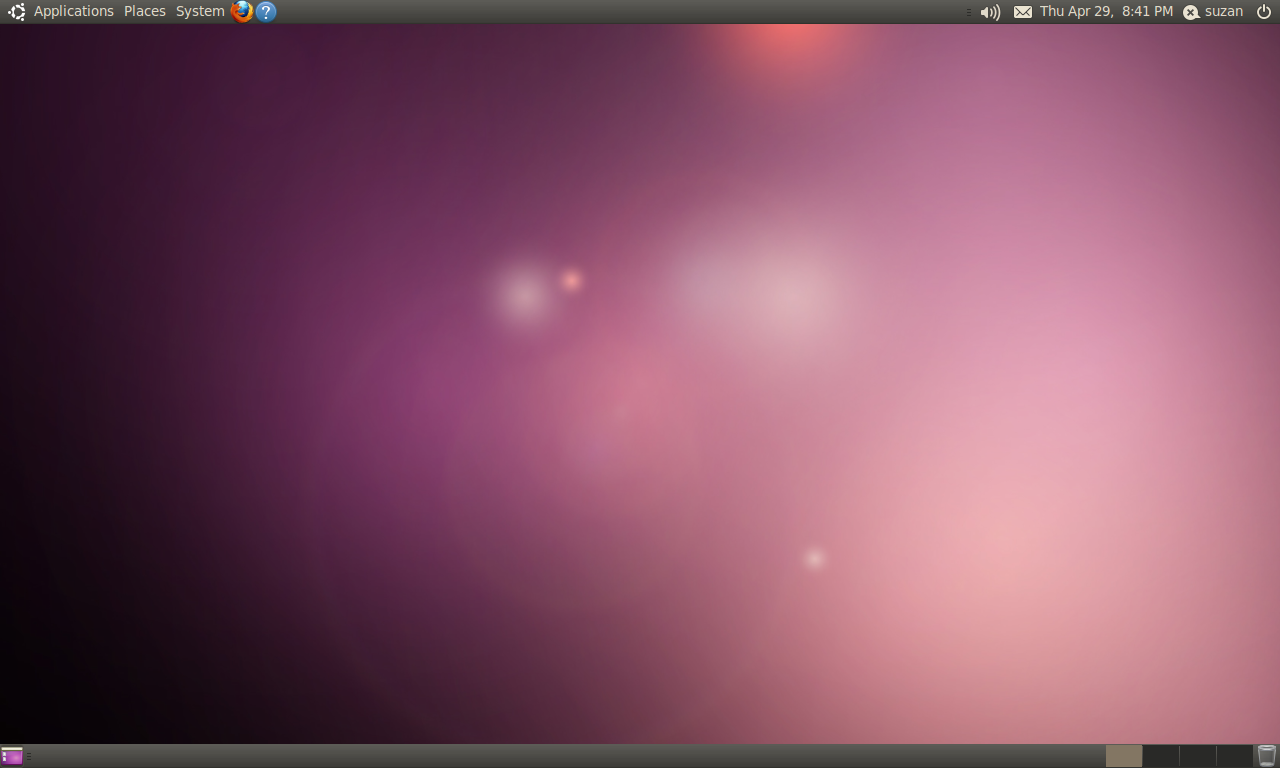
\includegraphics[width=400pt]{./images/ubuntu10-04.png}
	\caption{Ubuntu 10.04 Desktop}	
	\label{fig:ubuntu10.04}		
\end{figure}

\par \noindent In this section, only the changes are listed. How these new components work are covered in the upcoming chapters. \\

\begin{description}
	\item [Unity Launcher and Dash] Gone are the old application, places and systems menu. This is now replaced by the Unity dash and the launcher. Chapter \ref{chap:unity} will explain how to use them. But for now, it is important to understand the difference in launching and running applications between 10.04 and 12.04. This is one of the most important change which requires some time to get adjusted to.
	
	\item [Global Menu] In a bid to save vertical space, global menus are now part of the default 12.04 install. By default the application title is shown but when you hover over the top panel the global menu of the focussed application is shown. These is done to present a clean top panel appearance. 
		
	\item [HUD] Heads Up Display (HUD) is a new way accessing the menu items that you are looking for. It is currently present as a compliment to the Global menu. In the future, it will also provide support for voice commands. For a better understanding of HUD, please refer to chapter \ref{chap:unity}.

	\item [Gnome 3] Gnome 3 is now the new development focus of Gnome. This essentially means that every Gnome distribution will eventually upgrade to this new toolkit. With this toolkit, some features that were part of Gnome 2 are no longer supported. One such example is applets. Applets can no longer be added to the top panel. In Ubuntu 12.04, these are replaced by indicators. Many applets have already been converted into indicators which can be installed easily.	
\end{description}

\begin{figure}[h!]	
	\centering
	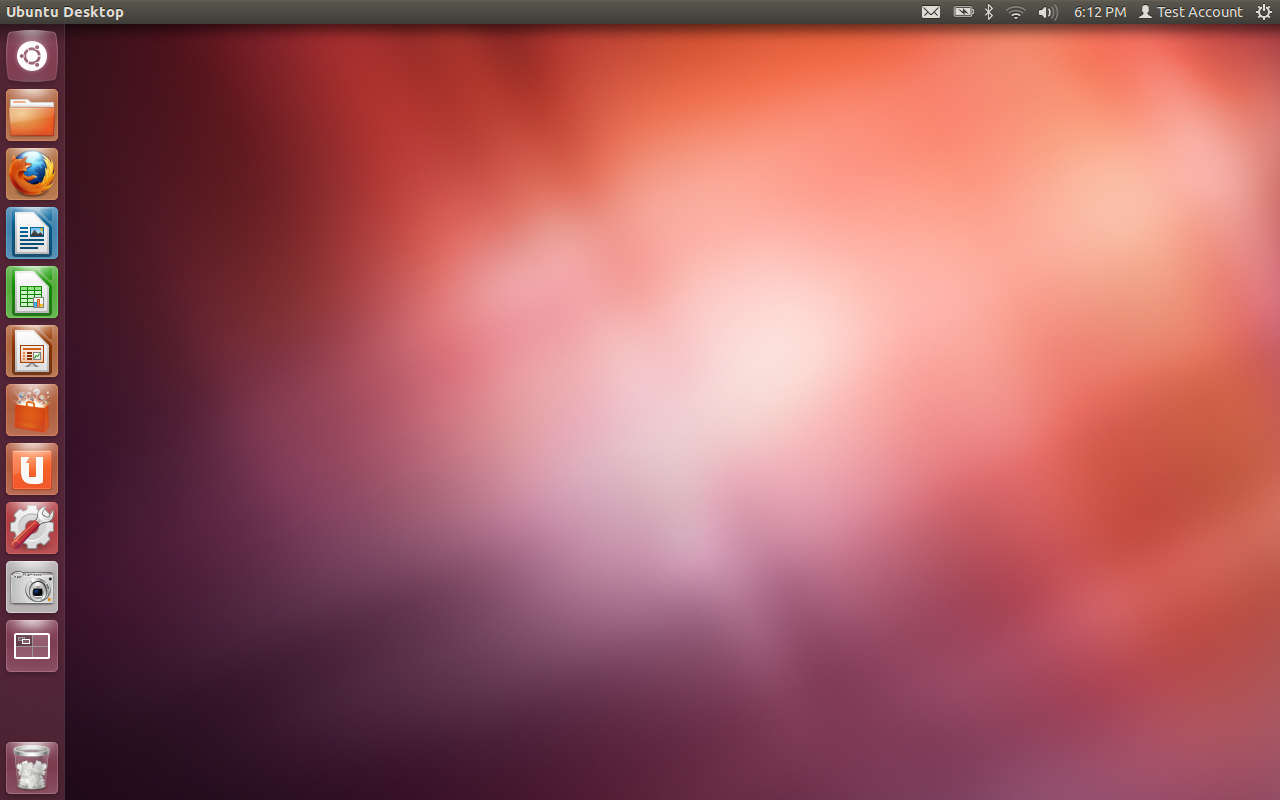
\includegraphics[width=400pt]{./images/ubuntu12-04.png}
	\caption{Ubuntu 12.04 Desktop}	
	\label{fig:ubuntu12.04}		
\end{figure}

\chapter{Note to Windows and Mac users} \label{chap:other-users}
This chapter is dedicated specifically to Windows and Mac users who are thinking of switching to Ubuntu. This chapter is intended to clear some myths and provide facts that you should consider before making this switch. 

\subsection*{1. An entirely different ecosystem}
When you switch from Windows or Mac OS to Ubuntu, remember that you are not just switching to another operating system but rather also an entire ecosystem of applications that was built for that operating system. In that sense, you were not using Internet Explorer, but rather \emph{Internet Explorer for Windows}. So do not be startled by the fact that Internet Explorer does not run in Ubuntu. Applications in Windows or Mac OS have been encouraged to be platform specific meaning it will only work in that specific operating system. This essentially locks you to Windows or Mac OS without so much of a choice. Use this opportunity to try out other open source applications such as Firefox, Libreoffice which are cross-platform, meaning they run on all operating systems such as Windows, Mac OS, Ubuntu (Linux). If you want to switch to Ubuntu, you need to break free of this dependency on Windows applications to use Ubuntu. The rewards of this are enormous as there are tons of applications out there.

\subsection*{2. The Anthropic principle}
By definition, everything you currently do in Windows works in Windows, otherwise you wouldn't have been able to do it. That doesn't mean that Windows does everything you might want it to do. In fact, if you really paid attention, you'd be aware of all of the things you wanted to do in Windows but couldn't. So the setup you have now is not necessarily the setup you want, it's just the one you settled for.  Since you are trying a switch to a different platform, now is the perfect time to question whether or not it's really what you want, or if you can do something better. Don't get stuck trying to re-create a solution you  used in Windows to a problem that doesn't actually exist on Linux. You have a whole world of new possibilities in front of you now, take advantage of that and question your old habits. For instance, Windows updates which roll out every now and then only include updates to the operating systems and other applications created by Microsoft like Windows Media Player. All the other applications installed by you are not updated and hence not up to date. This might be acceptable but a more desirable solution would be to update all the applications on your system in just one go. 

\subsection*{3. Look before you install}
If you look at typical fresh install of Windows for instance, you are presented with the bare necessary software pre-installed. Windows by default does not come with an office suite, Winzip utility etc. Because of this, Windows users generally have a habit of approaching a new installation with the desire to install more stuff. Ubuntu is different, and comes with a very large selection of useful applications already installed. So before you go off looking for an installer for Office, AIM or WinZip, look at what you already have because there is a good chance something is already there (LibreOffice, Empathy, File Roller).

\subsection*{4. The need to learn to use Ubuntu}
Accept the fact that Ubuntu is different from other operating systems. This does not essentially mean that you have to relearn every aspect of using your computer from scratch. It is true that you may have to relearn certain aspects, however this is entirely normal. This is something which can be seen everywhere. Imagine a Windows user trying to use Mac OS for the very first time. It will take time before you get used to the various touch gestures, the way of installing applications in Mac OS and file structure etc. The same applies when you switch to Ubuntu.  That said, this sole purpose of this manual is help you in this area. 


\part{Preparing Ubuntu}

\chapter{About Ubuntu} \label{sect:about-ubuntu}
% First write a small introduction about what is ubuntu like it being the 3rd best operating system in the world etc..
This chapter is intended to provide a small background about Ubuntu. Section \ref{chap:about_ubuntu_why} explains why a user should use Ubuntu since this will define the purpose and reason for a user. Section \ref{chap:about_ubuntu_who} digs a little deeper to describe the people behind Ubuntu. Section \ref{chap:about_ubuntu_release} explains in great detail how the Ubuntu release system works and the difference between different types of Ubuntu releases. This chapter ends with a section dedicated to learning to contributing back to Ubuntu.

\section{Why Ubuntu?} \label{chap:about_ubuntu_why}
% Explain the benefits of using ubuntu like opensource, secure, social, free, multiuser environment, cheap, effective etc...
This is certainly a valid and important question before proceeding to the rest of this manual. Why Ubuntu? Current Ubuntu users would cite various reasons for this from the freedom of choice to it being free. But let's go through the main reasons why you should definitely give Ubuntu a serious try.

\begin{description}
\item [Free] Ubuntu is and will always be free in the future. Ubuntu is developed by people all over the world embracing the principle of Free libre open-source software (FLOSS). This enables new software and updates to be available free of cost since they are written by volunteers and also the employees of Canonical, the parent company of Ubuntu. The code goes through an extensive review before they are uploaded to maintain the quality of the code.

\item [No Viruses] While using Ubuntu, you do not need to worry about installing any anti-virus programs since Ubuntu is completely free of viruses. Any security risks are fixed immediately due to an active community of Ubuntu users. 

\item [Community Support] When you need help using your system, the community is available everywhere around you to support you at all times. All this are done voluntarily by people passionate about Ubuntu. This Ubuntu manual you are reading is a proof of this statement. 

\item [Up to date software] Ubuntu will always be up to date with updates released regularly to ensure that your system is secure and bug free. These regular updates will be always be available for free. You will be notified automatically when updates are available.

\item [Beautiful, Polished, Stable] These are the goals of every Ubuntu release. Your Ubuntu is designed with the help of the community and experts after extensive discussion. Ubuntu is regularly user tested to ensure that it is easy and simple to use while preserving its elegance and polish.
\end{description}

\section{Who is behind Ubuntu?} \label{chap:about_ubuntu_who} \index{Mark Shuttleworth}
% List out the founder of Ubuntu, the ubuntu team, community, and its connection to Debian
Ubuntu was founded by Mark Shuttleworth, a South African entrepreneur coming up with their first release Ubuntu 4.10 codenamed Warty Warthog in October 2004. Ubuntu is backed by its parent company Canonical, also created by Mark Shuttleworth. Contributions to Ubuntu are shared by Canonical, other companies and the thousands of volunteers who bring their expertise to develop Ubuntu. Community members start small but gradually get more responsibility by earning the respect of the community. In short, Ubuntu is a community driven open source project. Ubuntu is built on the Debian base which in itself is strongly backed by the community.


\section{Ubuntu Releases} \label{chap:about_ubuntu_release} \index{Ubuntu Release Cycle}
% 6 months cadence, normal releases, LTS, support
Before proceeding to explain about how Ubuntu is released, it would be good to understand the meaning of the word \emph{cadence}.Cadence on its own means balanced and rhythmic flow. What does cadence mean in the world of Ubuntu? Quoting Ubuntu's founder Mark Shuttleworth, "Cadence is about releasing on a predictable rhythm." The Ubuntu team maintain a precise time rhythm in releasing a new version of Ubuntu. They release a new version of Ubuntu every six months. Let's now continue with the different types of Ubuntu releases.\\

\par \noindent As usual there is a new Ubuntu release every six months. However, not everyone would like to upgrade their system every six months. With this in mind, Ubuntu has two types of releases or should we say two versions of a release. There is a so called Long-Term-Support release (LTS) and normal releases. Cadence remains but types do change. Every two years there is a LTS release and in between these two years there are normal releases as usual. So the order of the release would be in the order shown in figure \ref{fig:ubuntu-release-cycle}. \\

\begin{figure}[h]	
	\begin{center}
	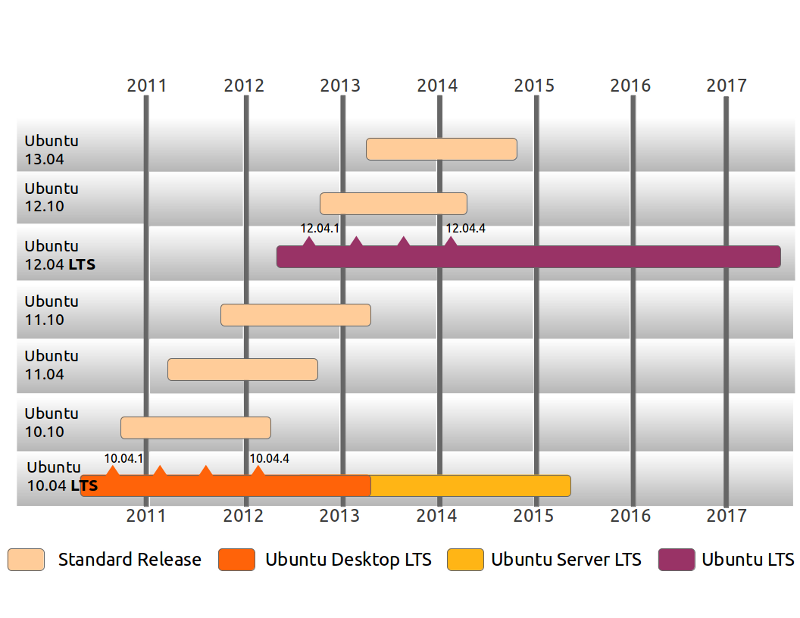
\includegraphics[width=300pt]{./images/about-ubuntu/ubuntu-release-cycle.png}
	\caption{Ubuntu Release Cycle}	
	\label{fig:ubuntu-release-cycle}	
	\end{center}
\end{figure}

\par \noindent Before explaining about the two types of a release, let us make a little digression and compare this with Windows updates since they can be compared with easily. When you have a fresh install of Windows on your computer you would have probably noticed that the system is constantly updated to get security patches and bug fixes. These are basically support provided by Microsoft. How long will one version of Windows receive updates depends on how long Microsoft decides to support its development and upgrade. This is similar with Ubuntu and the two mentioned types of a release. Only here Canonical  decides how long an Ubuntu release is supported. \\

\par \noindent Long-Term-Support (LTS) releases of Ubuntu are claimed to be stable versions since they are supported by Canonical for five years. So, you can practically use them on your computer for five years of no worry. After that time, you will no longer receive security updates and is recommended to a new release of Ubuntu.\\

\par \noindent On the other hand, Normal releases are supported for eighteen months. This type of release is targeted at users who like to constantly update to get the latest features. While LTS releases are targeted at corporations and users who would like to stick to one release for as long as they can while still being supported.\\

\par \noindent To summarize everything mentioned above, you can see the Ubuntu release chart in figure \ref{fig:ubuntu-releases} from the very first start of the Ubuntu project. \\

\begin{figure}[h]	
	\begin{center}
	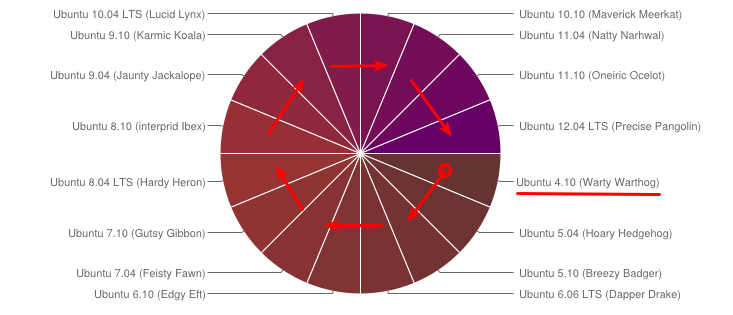
\includegraphics[width=400pt]{./images/about-ubuntu/ubuntu-releases.png}
	\caption{Ubuntu Releases}	
	\label{fig:ubuntu-releases}	
	\end{center}
\end{figure}

\par \noindent Let's explain figure \ref{fig:ubuntu-releases} briefly. The Ubuntu project started in the year 2004. You can see that by looking at the numbers after Ubuntu (e.g. 4.10, 5.04). The first number represents the year while the last two numbers represents the month of a year. Therefore, Ubuntu 4.10 was released in the year 2004 in October, Ubuntu 5.04 is released in the year 2005 in April and so on. \\

\par \noindent You would have also probably noticed that every release has an animal with an agnomen label (hint- Warthy Wartog). These are just code names of a certain release. It's something that Mark Shuttleworth came up with. The name stronly co-relates to the goals of that release. In this case, Ubuntu 12.04 is called Precise Pangolin because the focus of this release to polish the existing features to precision. For further reading, you are directed to see this youtube video here, where you can actually see what Mark Shuttleworth said about Ubuntu 10.04 Lucid Lynx (\href{http://www.youtube.com/watch?v=l02bhwofEqw}{Ubucon2009}). \index{Ubucon 2009}\\

%\section{Ubuntu derivatives} \label{chap:about_ubuntu_derivatives}

%\par \noindent In chapter \ref{chap:about_ubuntu_who}, you found out that Ubuntu is not a "stand alone" project in the open source world. More precisely, in the world of open source distributions development (hint- Torvalds, other distros, Debian, forks of distros). \\	% Need to be completed

%\par \noindent \textit{This section needs fixing.} These Ubuntu derivatives you can see as  forks, (not something you eat with), of Ubuntu. You can actually connect that with math (derivatives). You derive number and you get some other but the base remains the same. So Ubuntu is the base and other distributions that are derived from it are derivatives. Therefore we have: Xubuntu, Kubuntu, Edubuntu, Goobuntu. Each distro is meant for something else and for some other audience (e.g. Edubuntu is meant for schools and education). 

\section{Contributing to Ubuntu} \label{chap:about_ubuntu_contribute} \index{Contribute}
% Talk about FOSS, anybody can contribute to Ubuntu.....encourage users...the community makes Ubuntu.
If you are new to the open source world, this might be a bit surprising for you. You can actually contribute to the Ubuntu project. Ubuntu development is not done behind closed doors like other operating systems for instance Windows, Unix and Mac OSX. Of course, there are main contributors like the Canonical employees, but as part of the Ubuntu community you can also contribute in certain ways. \\

\par \noindent Certain ways to contribute to Ubuntu are,

\begin{description}

\item [Spread the word about Ubuntu] The easiest and simplest way to contribute to Ubuntu is to let everyone know about Ubuntu. Currently, one of the major stoppers towards widespread use of Ubuntu is the lack of awareness of Ubuntu. You can play an important role in solving this problem by organising Ubuntu release parties or by just word of mouth.

\item [Submit bug reports] While using Ubuntu if you encounter any bug, submit a bug report so that the Ubuntu developers are aware of the issue. All bugs are reported and tracked in \href{https://launchpad.net/}{Launchpad}. It is a bug tracker that aids the software team to collaborate on bug reports and provide fixes. You can submit bug reports via the terminal and the dash (you'll find out about terminal more later by reading this manual). You can read more about this in section \ref{sect:bugreport-terminal}.

\item [Involve yourself in Ubuntu development] After you get more comfortable with Ubuntu, you might have a wish to aid in developing it someday. Ubuntu has many projects like desktop, server, kernel etc. Contributing to Ubuntu development can take place in various levels. You can help by being a translator, programmer or by contributing as graphic designer. The options are endless. You can read more about contributing \href{http://developer.ubuntu.com/}{here} \index{Developer}.

%%Here is also more material for further readings, where you can actually learn about packaging which is very important part of an Ubuntu project. (Packaging tutorial for beginners).
\end{description}

\par \noindent In the open source world you always start as a volunteer. Starting small, you can gradually climb the ladder from being a volunteer to perhaps an Ubuntu Member or a Canonical employee. Linus Torvalds started working on his pet project. This project turned big to be called the Linux kernel which can now be found everywhere from mobiles, computers to small chips. As one of the main Linux kernel maintainers, namely Greg Kroah-Hartman, said: "Once I was doing this for a hobby. Now I don't have a hobby."  \\

\par \noindent Its entirely up to you. It is Free libre open-source software (FLOSS). You can decide if you want to contribute to the open source world and continue the FLOSS philosophy. That means that you can help it grow and develop. You can even fork Ubuntu, change it to your liking and share it with others. With open source you are not tied with licences, patents or any other kind of constrictions. 

\chapter{Obtaining Ubuntu} \label{sect:obtain_ubuntu}
In this chapter, let's look into how to obtain Ubuntu. First, the different steps to obtain Ubuntu are described in section \ref{sect:obtain_ubuntu}, after which some preparatory steps to transfer Ubuntu to a removable medium like a CD or a USB are discussed.

\section{Downloading Ubuntu} \label{sect:obtain_ubuntu} \index{Download Ubuntu}
As described in chapter \ref{sect:about-ubuntu}, Ubuntu is a open source operating system. This means that anyone can distribute Ubuntu. However, for safety reasons it is always advisable to obtain Ubuntu through official channels. There are 3 different ways in which this can be achieved. It is possible to download Ubuntu from the official website through a direct link, a torrent file or by buying a CD.

\subsection*{Direct Link} \label{sect:obtain_ubuntu_direct} \index{Download Ubuntu!Direct Link}
You can download Ubuntu directly from their official website \href{http://www.ubuntu.com/download/ubuntu/download}{\textit{here}}. You press on the big orange button to start the download as can be seen in figure \ref{fig:direct-link}. By default, the Ubuntu website shows the latest release which in this case is Ubuntu 12.04. 32-bit is officially recommended. If you are not sure of what 32-bit or 64-bit means, it is best recommended to not change any option and just press Start Download.\\ 

\par \noindent Once pressed, it will download the latest Ubuntu version and save it as a \emph{ISO} file. The \emph{ISO} file is basically an archive file which you can burn to a CD using your favourite CD burning program. 

\begin{figure}[h]	
	\begin{center}
	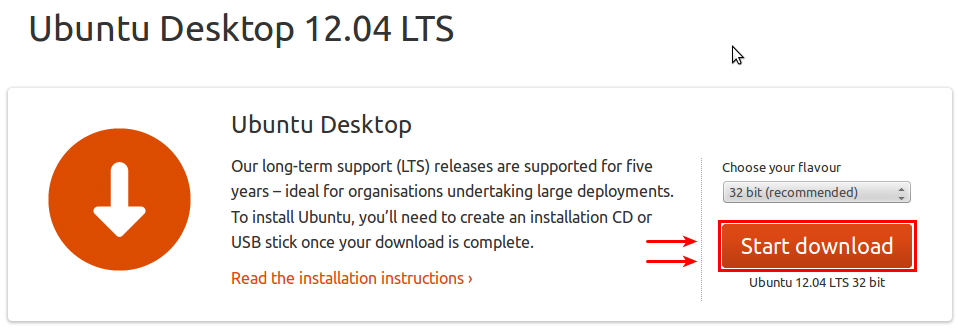
\includegraphics[width=400pt]{./images/obtain-ubuntu/direct-link.png}
	\caption{Direct link download}	
	\label{fig:direct-link}	
	\end{center}
\end{figure}


\subsection*{BitTorrent} \label{sect:obtain_ubuntu_torrent} \index{Download Ubuntu!Torrent}
BitTorrent is a peer-to-peer download network that sometimes enables higher download speeds and more reliable downloads of large files. You will need to install a BitTorrent client on your computer in order to download Ubuntu through this method. You can find all the bittorrent links \href{http://www.ubuntu.com/download/ubuntu/alternative-download}{\textit{here}}.

\subsection*{Buy CDs} \label{sect:obtain_ubuntu_buycd} \index{Download Ubuntu!Buy CD}
If you have a slow internet connection you can always choose to buy the Ubuntu CD and have it shipped to you. However, note that the official CD are only available after a few weeks after a new Ubuntu release. You can buy the CD \href{http://www.ubuntu.com/download/ubuntu/cds}{\textit{here}}. Remember that Ubuntu is completely free. The price covers the production cost of the CDs, includes applicable VAT, postage and packaging only.

\section{Burning Ubuntu to CD} 
When you download Ubuntu using a direct link or using a torrent as described in section \ref{sect:obtain_ubuntu_direct} and \ref{sect:obtain_ubuntu_torrent}, you finally are presented with a ISO file. Unlike a regular data file, the ISO file cannot be simply dragged and dropped or copied directly onto a disc. It needs to be burned in a specific way that expands/extracts the image so you have usable files on your disc. You can find detailed instructions on how to burn this ISO file into a CD \href{https://help.ubuntu.com/community/BurningIsoHowto}{here} and \href{http://www.ubuntu.com/download/ubuntu/download}{here}. The link provides instruction for Windows and Mac OS users as well.

\section{Create a bootable USB disk} \index{Bootable USB Disk}
In previous chapter you have learned how to make a bootable CD. The story in this section is pretty much the same (actually it's purpose is the same).  The main difference is the media used namely USB stick and BIOS adjustment (removable media has to be on the first place not CD or DVD). If you have a new computer then you might see something like USB CD or DVD  together. In older computers, label in BIOS  is just removable media.  Important to mention, computers that are built before 2001 probably won't have USB listed on a boot device priority. \\

\par \noindent Platform that is going to be used here to make a bootable USB is prior LTS version Ubuntu 10.04 Lucid Lynx. Before you go further be sure that you have USB that holds 2 or more GB of capacity. You can refer \href{http://www.ubuntu.com/download/ubuntu/download}{here} for more information about creating a bootable usb disk for other operating systems.\\

\newpage
\par \noindent Steps to make a bootable USB stick are: \\

\par \noindent 1. Connect your USB to your computer.\\

\par \noindent 2. Run the Startup disk creator application as shown in figure \ref{fig:usb2}. \\

\begin{figure}[h!]	
	\begin{center}
	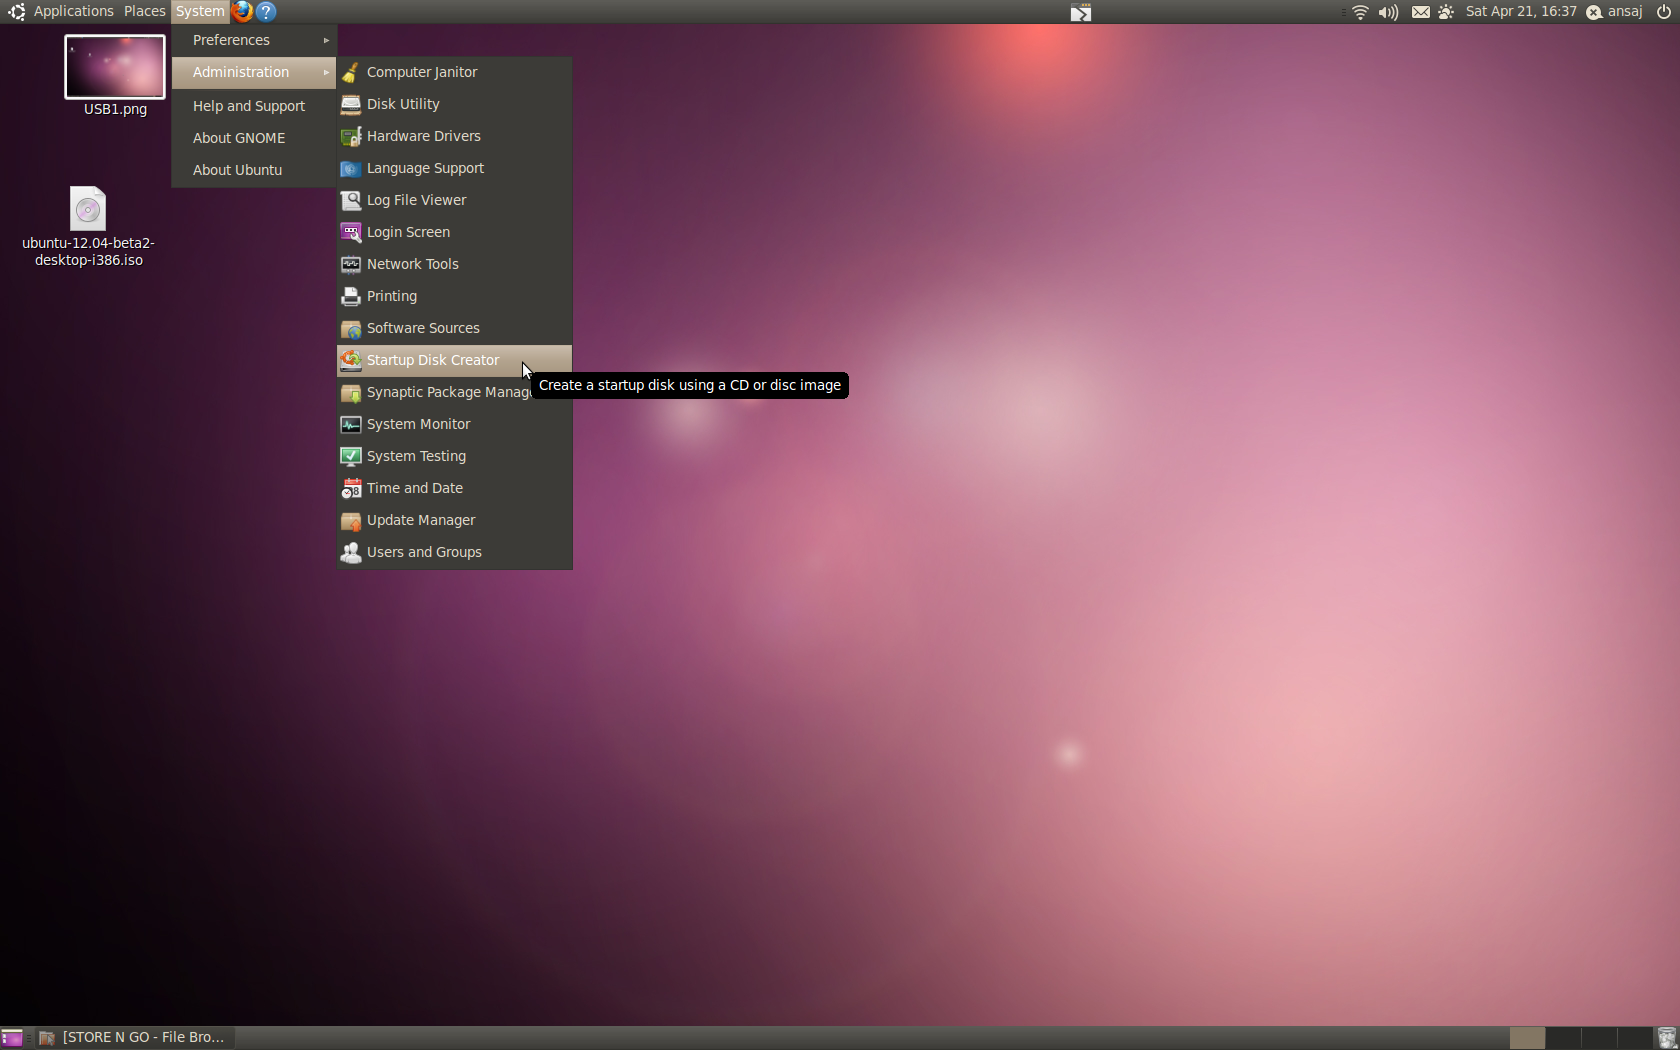
\includegraphics[width=400pt]{./images/obtain-ubuntu/USB2.png}
	\caption{Direct link download}	
	\label{fig:usb2}	
	\end{center}
\end{figure}

\par \noindent 3. After you have started application mentioned in a previous step, you should see something like figure \ref{fig:usb3}. You will notice that application recognized your media (USB) \\

\begin{figure}[h!]	
	\begin{center}
	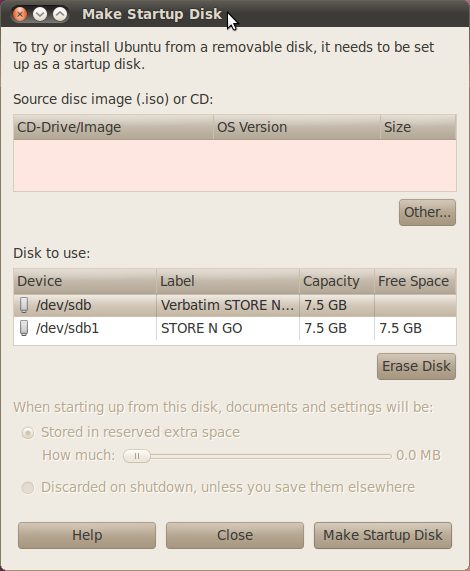
\includegraphics[width=200pt]{./images/obtain-ubuntu/USB3.png}
	\caption{Direct link download}	
	\label{fig:usb3}	
	\end{center}
\end{figure}

\par \noindent 4. Choose your ISO image (depends where you downloaded it or put it). In this example, the ISO is in the desktop. You have to click on the button Other like shown in previous illustration  so you could choose the ISO image. \\

\begin{figure}[h!]	
	\begin{center}
	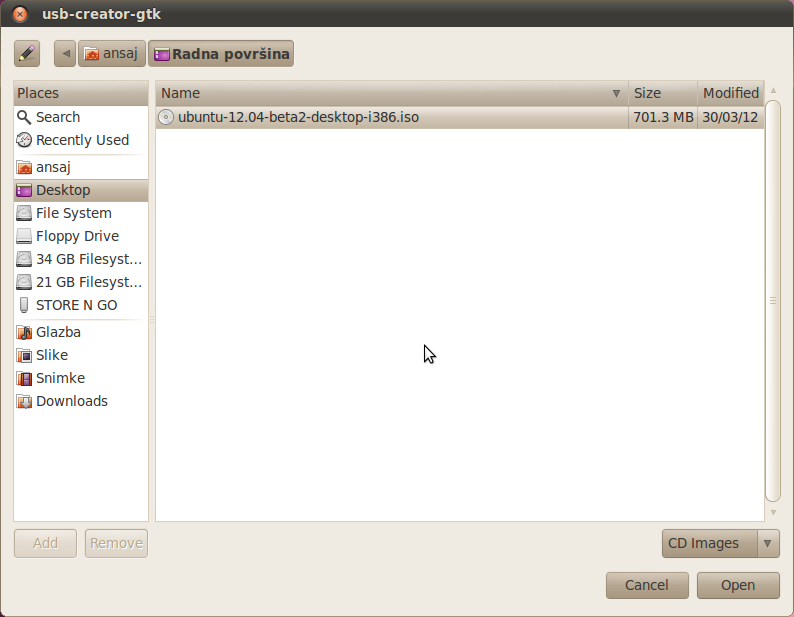
\includegraphics[width=300pt]{./images/obtain-ubuntu/USB4.png}
	\caption{Direct link download}	
	\label{fig:usb4}	
	\end{center}
\end{figure}

\par \noindent 5. After you have chosen the ISO and media, all you have to do is to click on a button  Make startup disk. Don't worry if you are prompted with authentication dialog-box. Just type in your administrator password. Be sure that you do it fast, otherwise you will have to repeat all the steps again. \\

\begin{figure}[h!]	
	\begin{center}
	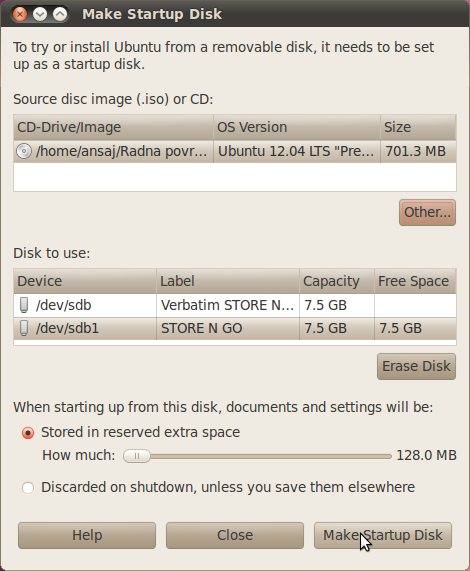
\includegraphics[width=200pt]{./images/obtain-ubuntu/USB6.png}
	\caption{Direct link download}	
	\label{fig:usb6}	
	\end{center}
\end{figure}

\par \noindent Now you will just have to wait until the tool converts your USB into a bootable USB.  After that you can just restart your computer and you are ready to try Ubuntu Live. You can even install it if you know further steps (Installation steps will be shown in the next chapter). Later on, if you decide that  you do not want to have a bootable USB anymore, just format your USB. 

\chapter{Installation} \label{chap:install}
% Installation chapter
You should have by now obtained the latest version of Ubuntu as described in chapter \ref{sect:obtain_ubuntu}. Its now time to try out Ubuntu on your system. If you have not installed an operating system before, do not worry since installing Ubuntu is extremely easy. The sections in this chapter are divided according to different case scenarios. This represents the first step in your journey into the world of Ubuntu. Let's try to make it as smooth as possible. Make sure to read this chapter carefully without skipping ahead.

\section{Prerequisite Steps}
Before proceeding to installing Ubuntu or any other operating system for that matter, it is necessary to make sure the following check list is complete. 

\subsection*{Check if your computer meets the minimum system requirements}
This is one thing which is often overlooked. The minimum system requirement to run Ubuntu with enough room to be comfortable are listed below. The best way to check is try out the Ubuntu Live CD. This is explained in section \ref{sect:live-ubuntu}.

\begin{itemize}
	\item 1 GHz CPU 
	\item 1 GiB Ram
	\item 15 GB Hard Disk Space
	\item 800 x 600 screen resolution
	\item Either a CD/DVD drive or USB port for the installation media
	\item Internet Connection
\end{itemize}

\subsection*{Know how to access your computer's BIOS}
It is necessary to know how to access your computer's BIOS. The BIOS decides which device to boot first. By default, it is set to boot from your hard disk since your current operating system is installed on your hard disk. However, since you are trying out a new operating system, you need to make the boot loader to boot from the CD first. \\

\par \noindent In order to access the BIOS setup, it is required to press a specific keyboard key. The keyboard key required to access your BIOS depends on your computer. You can check \textit{Appendix C} for the keyboard key you need to press for your system. If your computer isn't listed, then you need to search for it online. Once you are in the BIOS setup, choose the CD or USB option and press enter.

\subsection*{Backup your data}
It is always recommended to back up all your personal data onto a separate external storage device as a backup. This is an important and crucial step to avoid loss of personal data in the case of an emergency.

\newpage
\section{Trying out Ubuntu Live} \label{sect:live-ubuntu}
At this point, you may or may not have made your mind about installing Ubuntu permanently to your system. You do not have to install Ubuntu in order to try it out on your system. You can try out Ubuntu using the Live CD option which lets you run Ubuntu on your system without actually installing anything. This is helpful in trying out if Ubuntu works smoothly on your system and to experience Ubuntu before installing it. \\

\par \noindent Follow the steps below to try out Ubuntu using the Live CD option, \\

\par \noindent 1. Insert the Ubuntu installation CD into your CD-ROM. \\

\par \noindent 2. Power on your computer. You need to access the BIOS setup to make the computer to boot from your CD rather than the hard disk.  \\

\par \noindent 3. On booting your computer you are presented with the screen as shown in figure \ref{fig:start-up} . If you do not see this, then your computer is still booting from the hard disk rather than the CD. \\

\begin{figure}[h!]	
	\begin{center}
	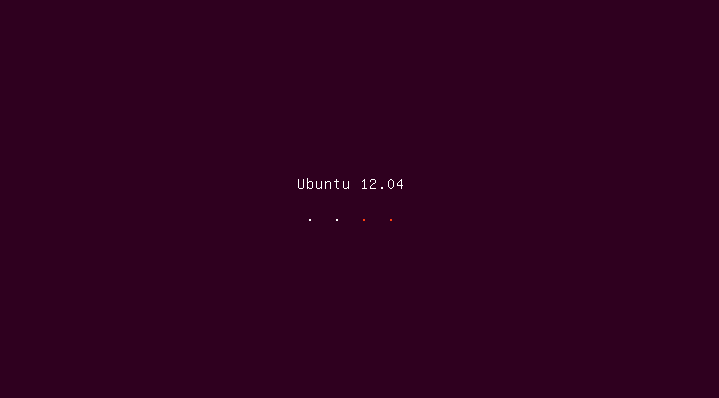
\includegraphics[width=300pt]{./images/installation/basic-start.png}
	\caption{Ubuntu start up screen}	
	\label{fig:start-up}	
	\end{center}
\end{figure}

\par \noindent 4. Wait for Ubuntu to start up. Once the loading is complete, you are presented with the dialogue box as shown in figure \ref{fig:live-options} where you can choose to Try Ubuntu first without installing anything.\\

\begin{figure}[!h]	
	\begin{center}
	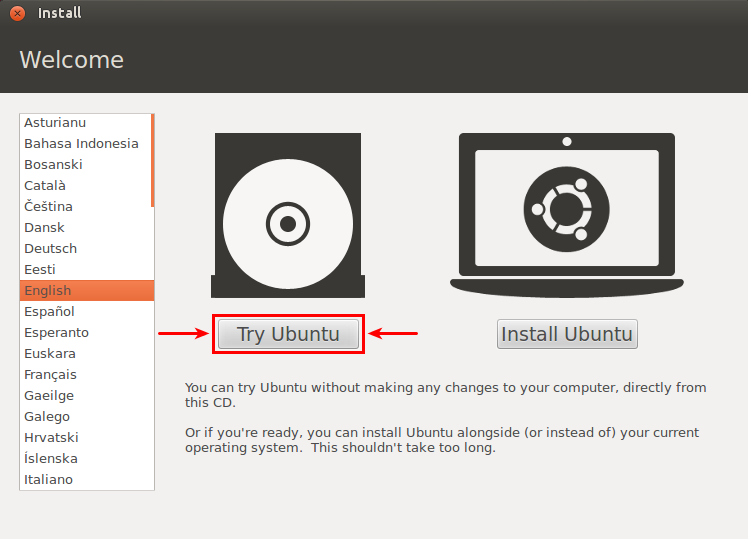
\includegraphics[width=300pt]{./images/installation/install-live-start.png}
	\caption{Try Ubuntu option}	
	\label{fig:live-options}	
	\end{center}
\end{figure}

\newpage
\par \noindent On choosing the "Try Ubuntu" option, you are presented with the Ubuntu desktop as shown in figure \ref{fig:live-desktop}. You can use Ubuntu to test out its features to your liking. You can browser the web, check your email and launch applications. If you like what you are using, you can choose to install it permanently by clicking on the Install Ubuntu 12.04 icon present on the desktop. It has been highlighted in figure \ref{fig:live-desktop}. The various installing steps are described in details in the following sections. \\

\begin{figure}[h!]	
	\begin{center}
	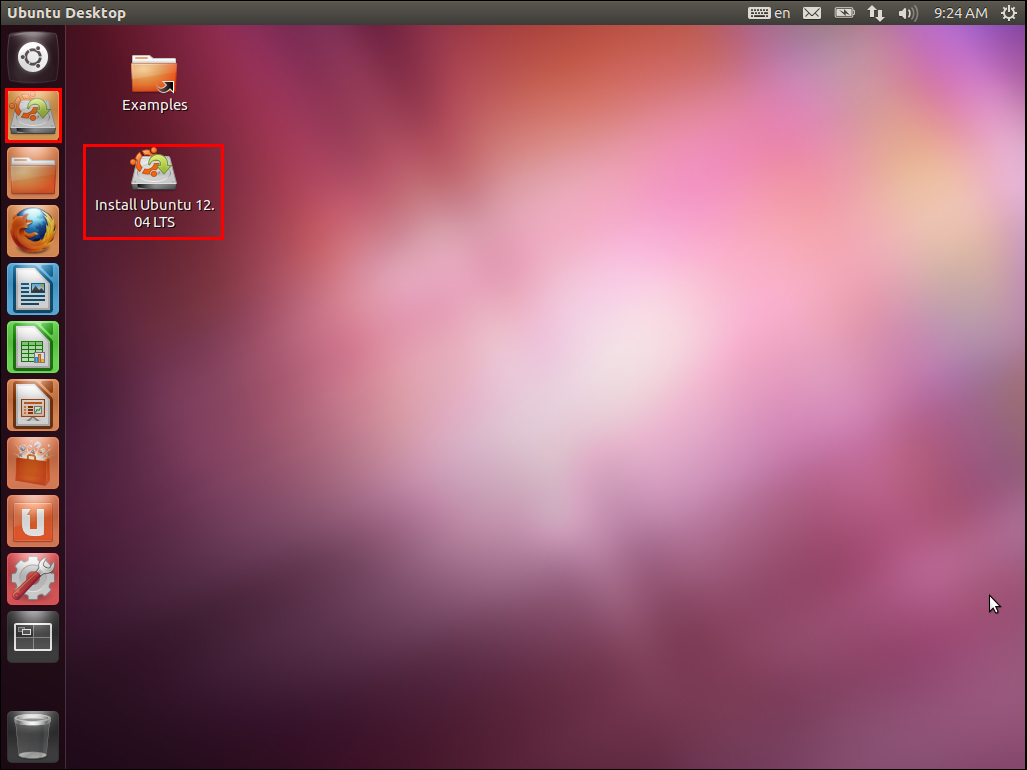
\includegraphics[width=400pt]{./images/installation/install-live1.png}
	\caption{Ubuntu Desktop}	
	\label{fig:live-desktop}	
	\end{center}
\end{figure}

\newpage
\section{Ubuntu as the only OS on the disk} \label{sect:ubuntu-install}
In the previous sections you read about how to run Ubuntu's live CD and what to do before you can actually install Ubuntu (e.g. backup your data, BIOS adjustment). Are you ready for the next step? If not, don't worry you can read the entire manual first, and when you are comfortable with everything you will be ready not just for the Ubuntu installation process but the usage too. If you are ready please be sure that you have done everything connected with steps before installation. If you haven't done everything, this is your last chance to do it before you go further. \\

\par \noindent As is mentioned earlier in this chapter, this section will describe how to install Ubuntu as the only operating system on your computer.This installation scenario is much easier than when considering to install Ubuntu alongside with Windows. All you have to be sure is that you have done the proper BIOS adjustment and backup of your data on to some external storage media like CD, DVD, USB or external disk.  \\

\par \noindent 1. Turn on the computer and insert the Ubuntu installation CD into the CD-ROM. Ensure that the BIOS is set to boot from the CD. Wait for the BIOS to read the CD and recognise the operating system. If everything is done properly you'll be able to see the Ubuntu start up screen as shown in figure \ref{fig:basic-start}.

\begin{figure}[h!]	
	\begin{center}
	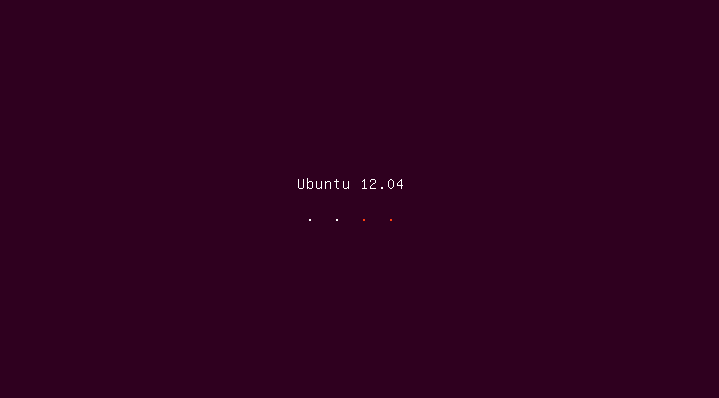
\includegraphics[width=300pt]{./images/installation/basic-start.png}
	\caption{Ubuntu start up screen}	
	\label{fig:basic-start}	
	\end{center}
\end{figure}

\par \noindent 2. Wait for Ubuntu to start up. Once the loading is complete, you are presented with the dialogue box as shown in figure \ref{fig:install-live-options} where you need choose to install Ubuntu. You can choose the installation language from the options shown on the left side.\\

\begin{figure}[!h]	
	\begin{center}
	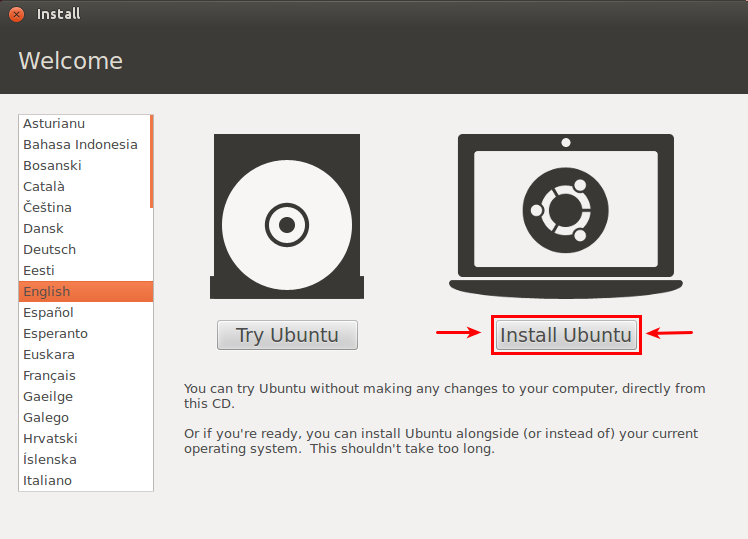
\includegraphics[width=300pt]{./images/installation/install-live-start2.png}
	\caption{Install Ubuntu option}	
	\label{fig:install-live-options}	
	\end{center}
\end{figure}

\par \noindent 3. Ubuntu checks if your system has access to the internet, connected to the power supply (laptop) and has atleast 4.4 Gb hard disk space. You will be also be required to choose if you want to install third party software and updates  during the installation. %Skip that part now because you can do that after you have installed it. 

\begin{figure}[!h]	
	\begin{center}
	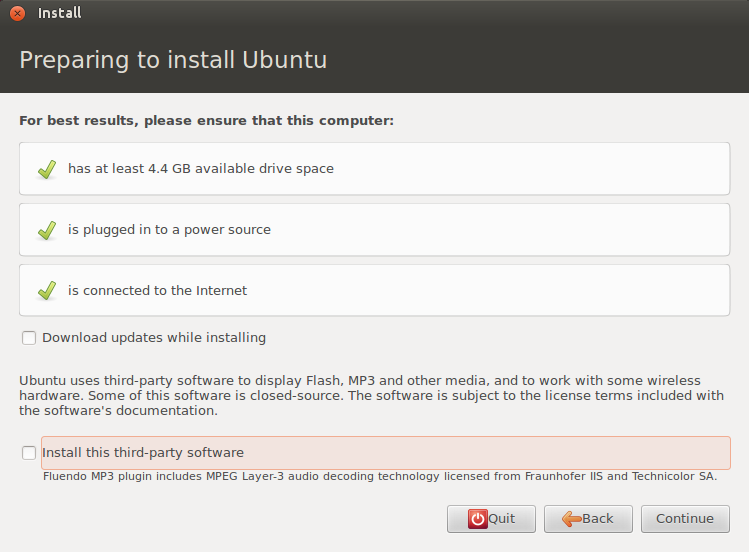
\includegraphics[width=300pt]{./images/installation/installer-prepare.png}
	\caption{Installer Options}	
	\label{fig:installer-prepares}	
	\end{center}
\end{figure}

\par \noindent 4. You are now presented with options to choose the type of installation you would like to perform. You can install Ubuntu alongside other operating systems (if you have any personal data, they will not be erased), Erase disk and install Ubuntu as the only operating system on your system or something else. If you have no other operating system installed on your system, then you will have only have the last two options. In this section which deals with Ubuntu as the only operating system, you need to choose the second option which removes any other operating system such as Windows XP, Vista or 7 and automatically does all the hard disk partitioning for you. \\

\begin{figure}[!h]	
	\begin{center}
	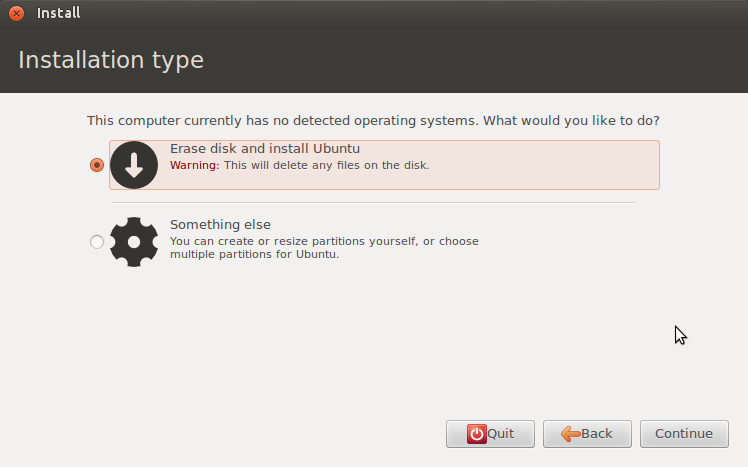
\includegraphics[width=300pt]{./images/installation/installer-os-options.png}
	\caption{Installer Options}	
	\label{fig:installer-prepare}	
	\end{center}
\end{figure}

\par \noindent On choosing the Erase disk and install Ubuntu option, you are presented with the following screen. Click on Install Now to start the Ubuntu installation. Note that this is permanent. If you click on Install Now, the installer erases all your data and installs Ubuntu! \\

\begin{figure}[!h]	
	\begin{center}
	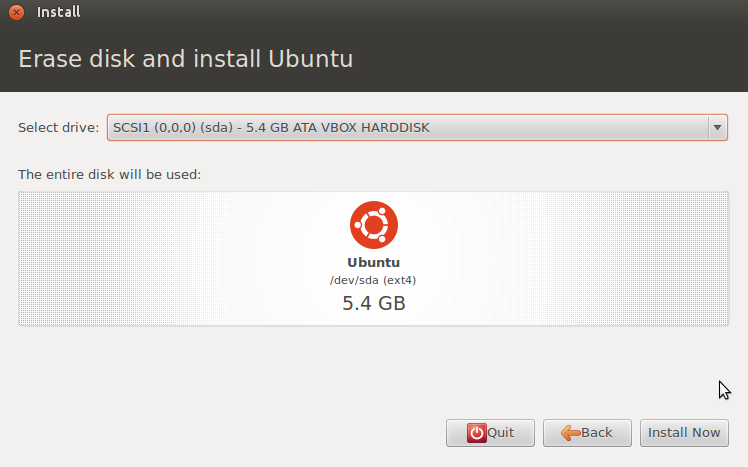
\includegraphics[width=300pt]{./images/installation/installer-onlyubuntu.png}
	\caption{Installer Options}	
	\label{fig:installer-onlyubuntu}	
	\end{center}
\end{figure}

\newpage
\par \noindent 5. The previous step was the hardest. Now it is basically entering some personal information. You first need to choose your keyboard layout. Ubuntu will automatically detect your keyboard layout. However, you can change the keyboard layout to match the local language settings. \\

\begin{figure}[!ht]	
	\begin{center}
	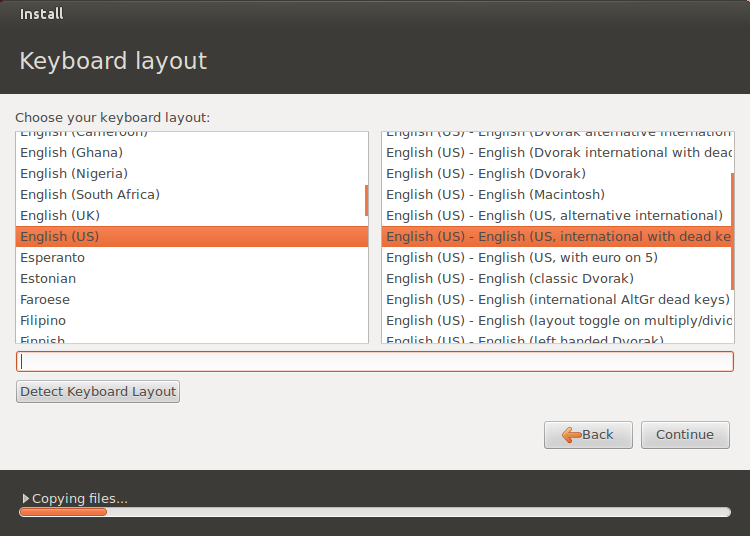
\includegraphics[width=300pt]{./images/installation/installer-keyboard.png}
	\caption{Installer Options}	
	\label{fig:installer-keyboard}	
	\end{center}
\end{figure}
\newpage
\par \noindent 6. You need to enter the place where you live. This is to automatically get the timezone and set the correct time. \\

\begin{figure}[!h]	
	\begin{center}
	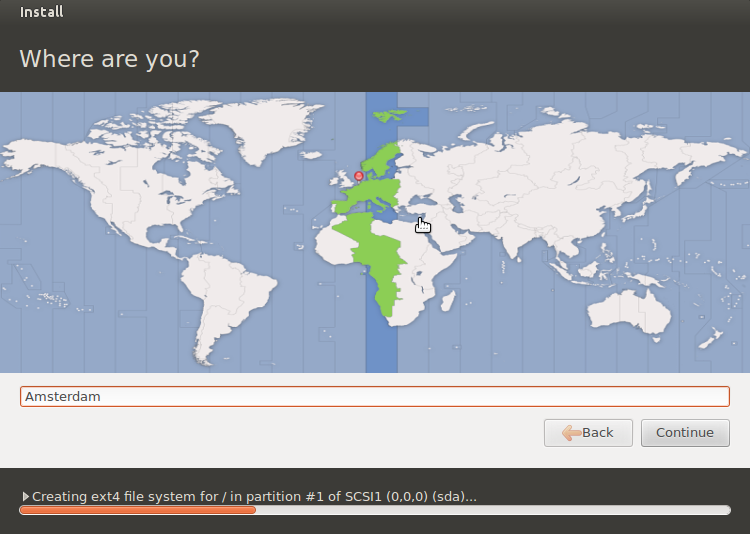
\includegraphics[width=300pt]{./images/installation/installer-timezone.png}
	\caption{Installer Options}	
	\label{fig:installer-keyboard}	
	\end{center}
\end{figure}

\par \noindent 7. The last step and this is where you set the username, password and other options like requiring a password to login in. \\

\begin{figure}[!h]	
	\begin{center}
	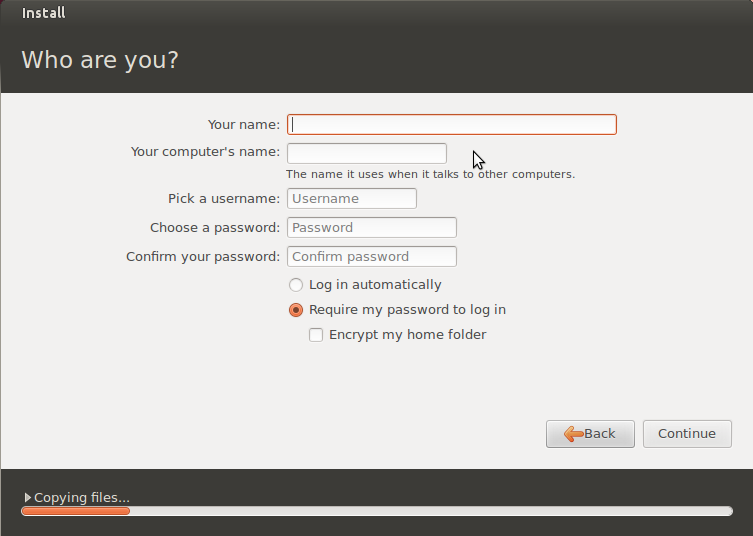
\includegraphics[width=300pt]{./images/installation/installer-who.png}
	\caption{Installer Options}	
	\label{fig:installer-who}	
	\end{center}
\end{figure}

\par \noindent After you have entered all the required data click on the button Continue and wait for around 20 minutes. After the installation is done, reboot your computer, take the CD out. The new operating system is waiting to be used. Congratulations on your Ubuntu install.

%\section{Ubuntu dual boot with Windows}
% This section needs to be added for the next edition perhaps.

\newpage
\section{Ubuntu on a virtual machine}
This section will describe how to try or install Ubuntu virtually without affecting your existing setup. By virtually running Ubuntu on a virtual machine, it is the same as you would use it if it was natively installed on your computer. Before proceeding, it is good to mention that you will need a spare 1 GiB of memory and atleast 8 GB of hard disk space. Then only can you actually run Ubuntu on a virtual machine. The virtually run Ubuntu is a guest operating system on your computer, and will use the same memory as your currently running operating system.  Hence you need memory for your current operating system plus memory for running Ubuntu. For instance, if you wanted to virtually run Ubuntu on a Windows Vista machine, you would need 2 GB (for Windows Vista) plus 1 GB (for Ubuntu) to use this method. For this example about how to setup a virtual machine, the application VirtualBox is used. You can  also use other alternatives namely, VMware, Parallels etc.  \\

\par \noindent 1. Open VirtualBox application, and left click on the New button as shown in figure \ref{fig:virtualbox-main} to start the virtual machine setup process. \\

\begin{figure}[!h]	
	\centering
	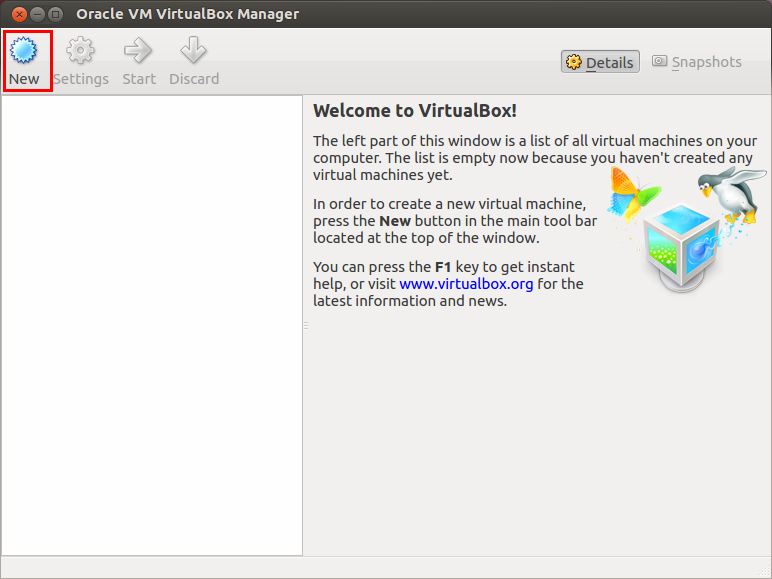
\includegraphics[width=300pt]{./images/installation/virtualbox/virtualbox-main.png}
	\caption{VirtualBox Manager main interface}	
	\label{fig:virtualbox-main}	
\end{figure}

\par \noindent 2. Type a virtual machine name. VirtualBox can automatically recognize the operating system you are going to use or install using the name. So if you type Ubuntu 12.04 LTS, VirtualBox will automatically fill in Linux and Ubuntu in the second and third blank box as shown in figure \ref{fig:wizard-newvirtual}. \\

\begin{figure}[!h]	
	\centering
	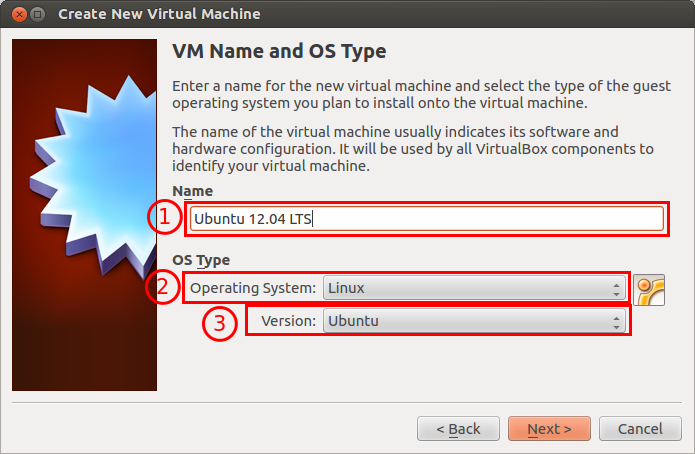
\includegraphics[width=300pt]{./images/installation/virtualbox/wizard-newvirtual.png}
	\caption{Virtual machine details}	
	\label{fig:wizard-newvirtual}	
\end{figure}

\par \noindent 3. Here you will have to give the guest operating system memory that it will use while running. It will use part of your memory that your current operating system already uses. It is recommended to atleast 512 MB (VirtualBox has already done that by default as seen in figure \ref{fig:wizard-memory}), but you can provide more if you have sufficient memory.  You will then just have to click on the button Next. \\

\begin{figure}[!h]	
	\centering
	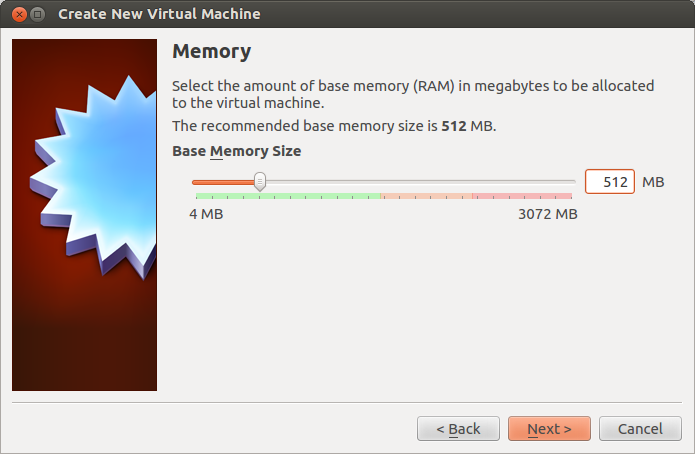
\includegraphics[width=300pt]{./images/installation/virtualbox/wizard-memory.png}
	\caption{Memory size for guest operating system}	
	\label{fig:wizard-memory}	
\end{figure}

\par \noindent 4. Here you will just have to give some disk space to the guest operating system. The minimum recommended is 8 GB as you can see in figure \ref{fig:wizard-newharddisk}.  Remember the concept of a hard disk for the guest operating system is virtual. In reality, you will be basically creating a file of the size 8 GB. This will in no way affect your current hard disk partitions. \\ 

\begin{figure}[!h]	
	\centering
	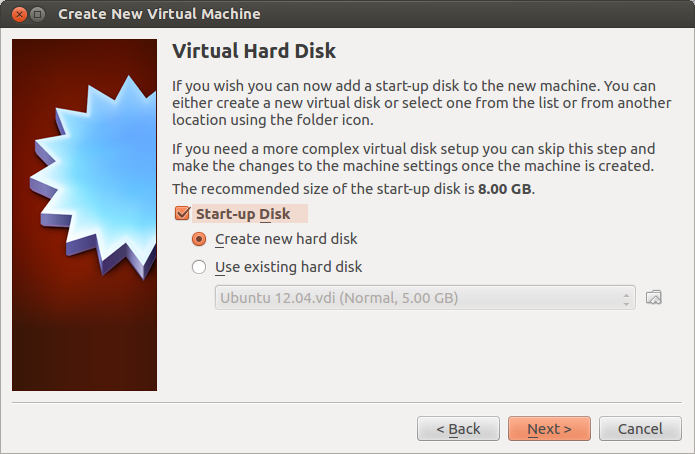
\includegraphics[width=300pt]{./images/installation/virtualbox/wizard-newharddisk.png}
	\caption{New startup disk}	
	\label{fig:wizard-newharddisk}	
\end{figure}

\par \noindent Click Next to proceed to create this file which will serve as a virtual hard disk for your guest operating system. Based on your disk space you can give it any value more than 8 GB.\\

\newpage
\par \noindent 5. In this step you will only have to choose the VirtualBox disk image and nothing else. VirtualBox does that already by the default as seen in figure \ref{fig:wizard-VDI}. \\

\begin{figure}[!h]	
	\centering
	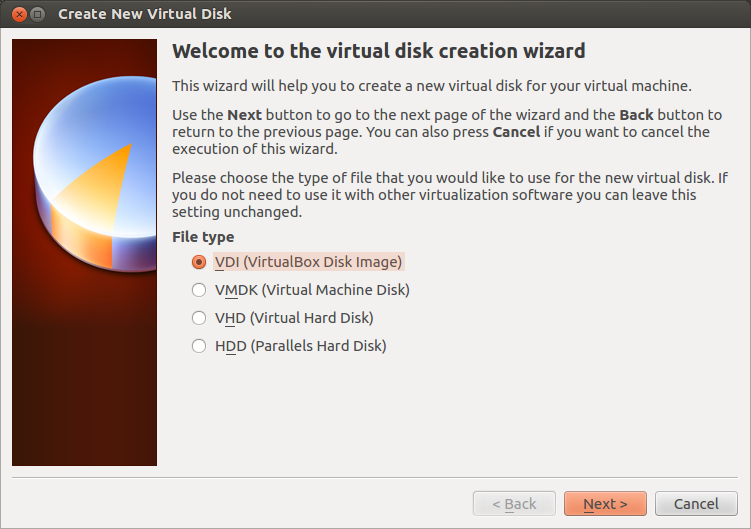
\includegraphics[width=300pt]{./images/installation/virtualbox/wizard-VDI.png}
	\caption{VirtualBox disk image}	
	\label{fig:wizard-VDI}	
\end{figure}

\par \noindent 6. Here you can choose to set the property of the new virtual disk. The virtual disk size can be dynamically allocated  or have a fixed size. Choose dynamically allocated as shown in figure \ref{fig:wizard-dynamicsize}. If you will use the new guest operating system for a while, there is a possibility that you will need space for new applications and the disk space required might grow. By choosing dynamically allocated size, you won't have to worry that your virtual machine might end up with lack of space. It will grow dynamically as the operating system grows. \\

\begin{figure}[!h]	
	\centering
	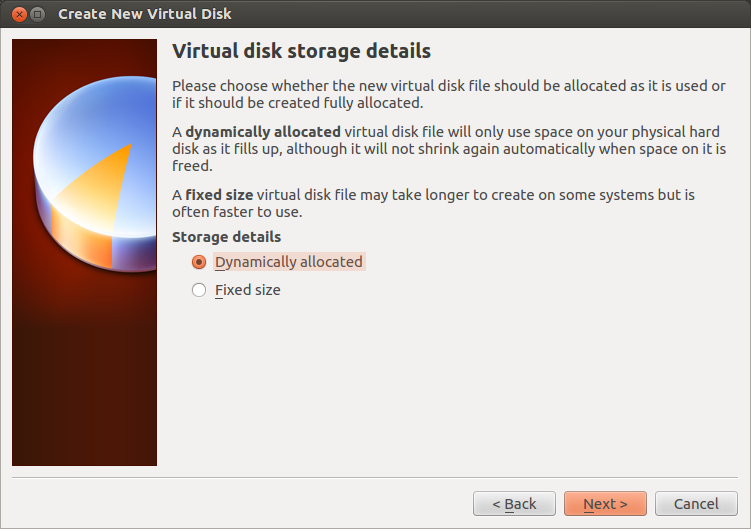
\includegraphics[width=300pt]{./images/installation/virtualbox/wizard-dynamicsize.png}
	\caption{VirtualBox disk storage details}	
	\label{fig:wizard-dynamicsize}	
\end{figure}

\newpage
\par \noindent 7. As seen in figure \ref{fig:wizard-newharddisk}, the minimum disk size for the guest operating system is 8 GB. As shown in figure \ref{fig:wizard-sizelocation}, you can set the virtual disk size from 8GB or more.  It actually depends on how much disk space you have at all.  \\

\begin{figure}[!h]	
	\centering
	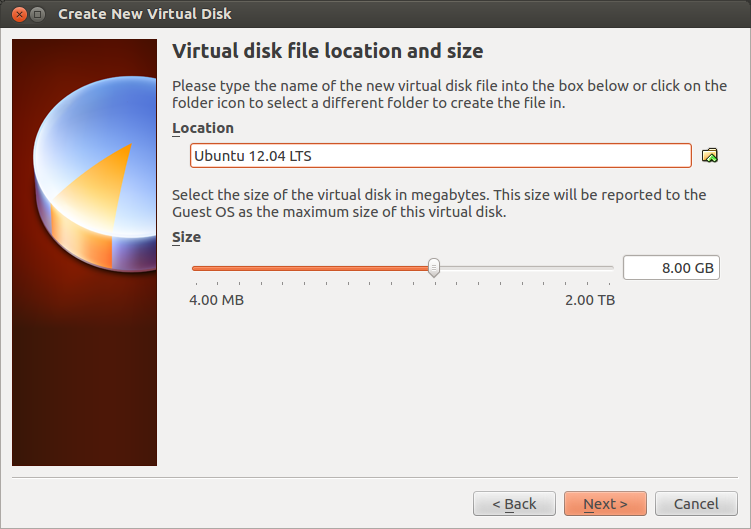
\includegraphics[width=300pt]{./images/installation/virtualbox/wizard-sizelocation.png}
	\caption{VirtualBox disk storage details}	
	\label{fig:wizard-sizelocation}	
\end{figure}

\par \noindent 8. Press Create to finish the wizard. You have now successfully created a virtual machine for running Ubuntu 12.04 LTS. With this you have created a virtual machine, but you still need to configure it and then actually perform the Ubuntu installation on the virtual hard disk.\\

\begin{figure}[!h]	
	\centering
	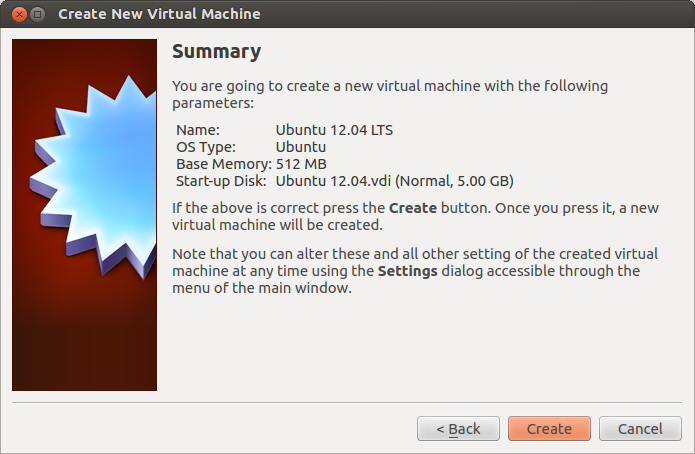
\includegraphics[width=300pt]{./images/installation/virtualbox/Wizard-complete.png}
	\caption{Wizard complete}	
	\label{fig:Wizard-complete}	
\end{figure}

\newpage
\par \noindent 9. With the wizard complete, you now need to configure the virtual machine before you can use it. This is illustrated below. Open the setting dialog by clicking the settings button as shown in figure \ref{fig:wizard-final}. \\

\begin{figure}[!h]	
	\centering
	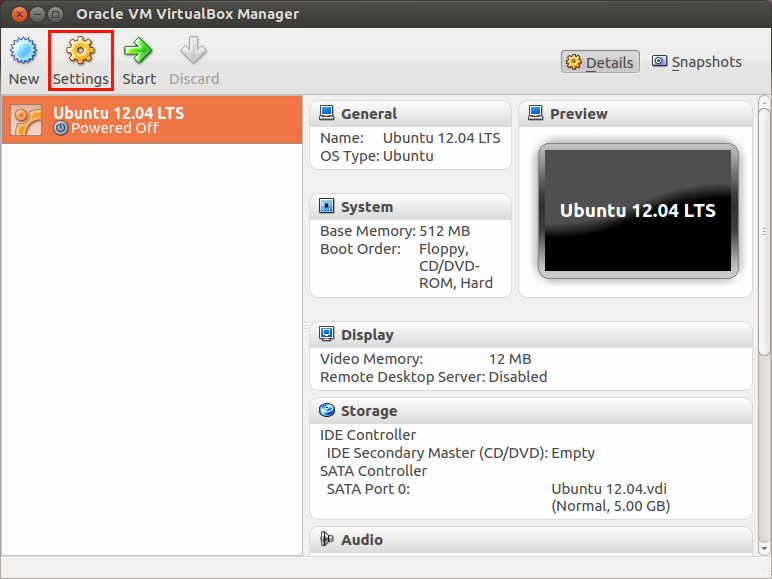
\includegraphics[width=300pt]{./images/installation/virtualbox/wizard-final.png}
	\caption{Click settings button}	
	\label{fig:wizard-final}	
\end{figure}

\par \noindent 10. Here you can adjust general stuff like virtual machine name to advanced things like sharing folders between your virtual operating system and natively installed operating system. The main focus here however is to change the display settings. First set the video memory to a value where Ubuntu can run reasonably well on your virtual machine. You could set it 128 MB or more preferable for better performance. Second, enable 3D acceleration. This is required to run Unity. You can see the steps illustrated in figure \ref{fig:settings-display}. \\

\begin{figure}[!h]	
	\centering
	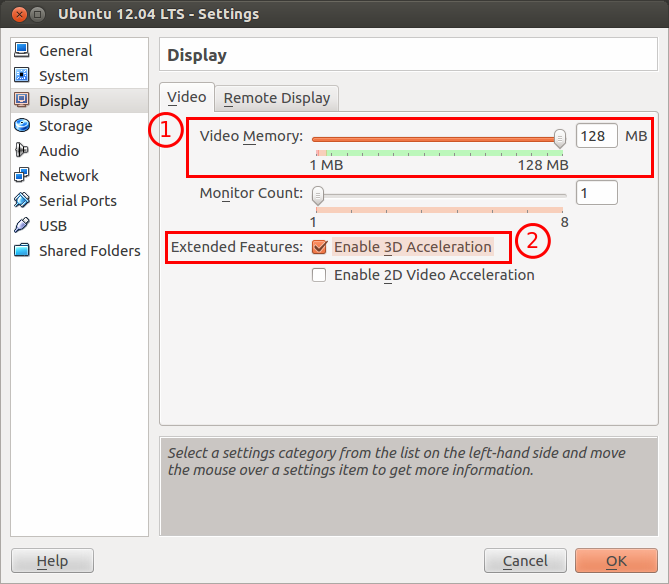
\includegraphics[width=300pt]{./images/installation/virtualbox/settings-display.png}
	\caption{Display settings}	
	\label{fig:settings-display}	
\end{figure}

\par \noindent 11. Finally, you need to provide the installation medium (in this case the Ubuntu ISO file) so that the virtual machine will try to install Ubuntu from this file. You can select the ISO file by clicking on the CD icon shown in 2nd box in figure \ref{fig:settings-storage}. \\

\begin{figure}[!h]	
	\centering
	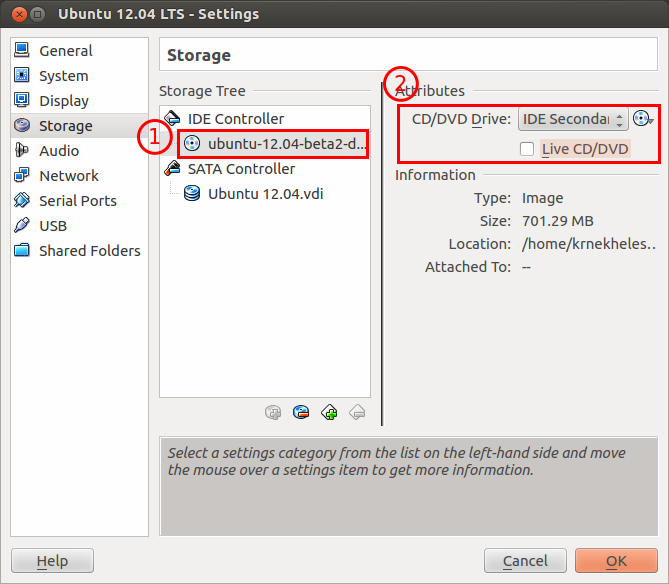
\includegraphics[width=300pt]{./images/installation/virtualbox/settings-storage.png}
	\caption{ISO File path}	
	\label{fig:settings-storage}	
\end{figure}

\par \noindent And that's it. You have completed configuring the virtual machine. Now close the settings dialog and click on the start button. The virtual machine will now open and you can proceed to install Ubuntu on the virtual hard disk from there. The entire Ubuntu installation process is already covered in section \ref{sect:ubuntu-install}. \\






\part{Using Ubuntu}

\chapter{The Unity desktop} \label{chap:unity}
Until now, it has all been about preparing and installing Ubuntu on your system. This chapter is more like an orientation session where the various elements of the Ubuntu desktop are introduced to get you acquainted to using Ubuntu. Figure \ref{fig:ubuntu-desktop1} shows the default Ubuntu desktop. \\

\begin{figure}[h]	
	\centering
	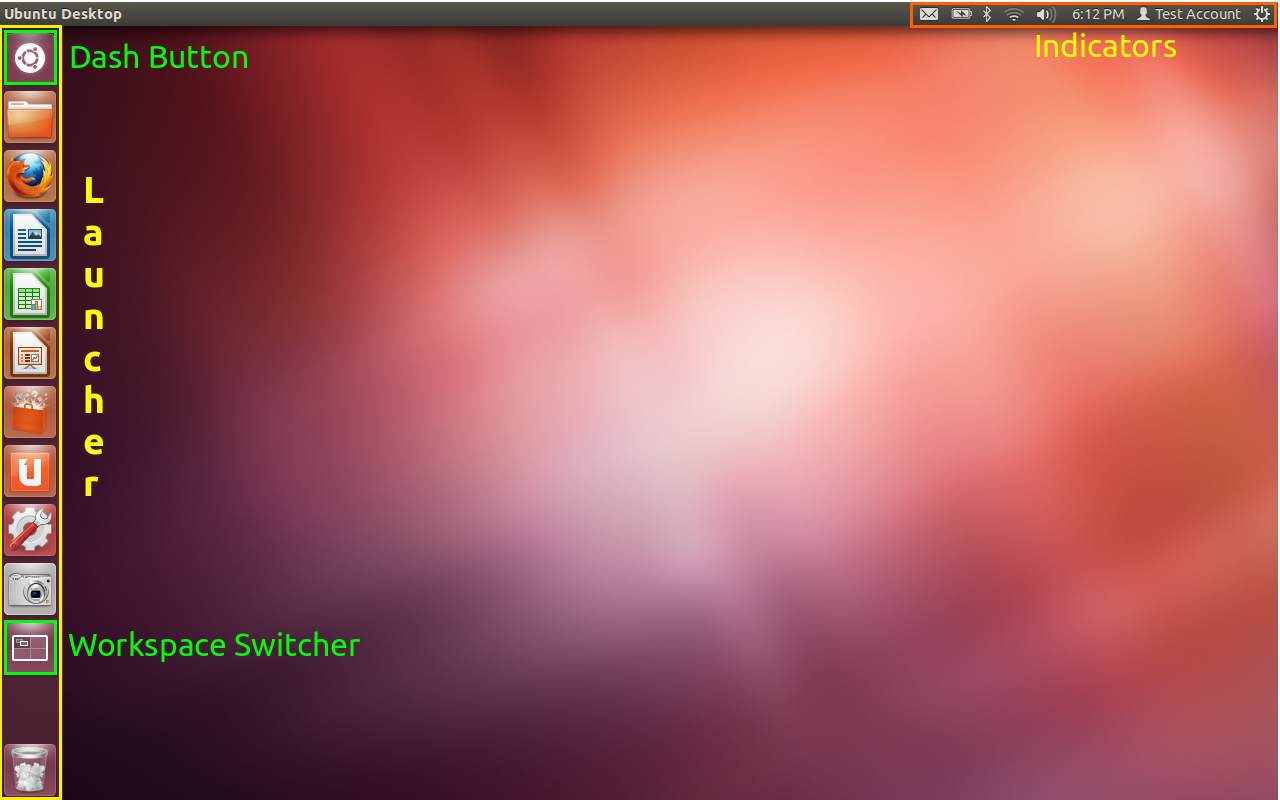
\includegraphics[width=400pt]{./images/desktop/desktop.png}
	\caption{Ubuntu Desktop}	
	\label{fig:ubuntu-desktop1}		
\end{figure}

\par \noindent Let's go through the various elements one by one starting with the launcher.  While describing the elements, it is also explained on how to use that element.

\section{Launcher} \index{Unity!Launcher}
The stack of icons on the left-hand side of the desktop (indicated by a yellow box) is called the Launcher. As the name suggests, its purpose is to help launch applications and performs the following functions.

\begin{itemize}
	\item Behave like a dock or start menu - You can pin your favourite applications for easy launch
	\item Shows the currently running applications
	\item Shows the status of the application (download progress, file copy progress etc)
	\item Shows external devices such as USB, external hard drive etc.
\end{itemize}

\par \noindent The launcher can be compared to the Windows Start panel or the Mac OS dock. You can launch an application by clicking on an application icon. If you want to remove the application  from the launcher, simply right-click the application icon and press ``Unlock from launcher".\\

\par \noindent The launcher also shows the currently running applications using small triangles. A white triangle is shown on the left side of an application icon to indicate that it is open. On the other hand, a white triangle is placed on the right side of the application if it is the currently focussed application. In figure \ref{fig:unity-applications}, the File manager and Firefox are open which is indicated by the white triangle on the left side of their icons. However, File manager is the application which is currently in focus, hence it also has a white triangle on the right side of its icon.

\begin{figure}[h]	
		\centering		
		\subfloat[State]
		{ 	\label{fig:unity-applications} 	
\includegraphics[width=40pt]{./images/desktop/applications.png} } 
		~ \hspace{1in}
		\subfloat[Move]
		{ 	\label{fig:unity-move-applications} 	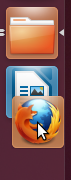
\includegraphics[width=50pt]{./images/desktop/move-applications.png}	}		
		\caption{Unity Launcher}
		\label{fig:unity-app}
\end{figure}

\par \noindent To indicate more than one instance of an application being open, two or three triangle depending on the number of instances appear on the left side of the icon. In figure \ref{fig:unity-move-applications}, there are two instances of the File manager open which is indicated by the two triangle to its left. You can also choose to rearrange applications in the launcher according to your preference. You can do this by pressing on the application icon, after a small delay the application slides out of its place as can be seen in \ref{fig:unity-move-applications}. You can now place it according to your preference. \\

\par \noindent The launcher can also be used to indicate the state, progress of an application. Basically the application icons indicate the progress of certain actions running in the background. This helps to keep track of the progress of an application action while actually working on something else. For instance, let's assume you are updating your system. You do not wait or keep checking the update manager to see if it is finished. You can meanwhile browse the web, check your email and keep an eye on the update manage application icon on the launcher. It shows the the number of updates and the update progress as seen in figure \ref{fig:update-number.png}. This is just one example. Several default applications in Ubuntu use this feature to display useful information using the launcher. Mozilla Thunderbird (default email client), Nautilus (default file manager) are few examples of such applications.\\

\begin{figure}[h]	
	\centering
	
\includegraphics[width=40pt]{./images/desktop/update-number.png}
	\caption{State, progress of the Update manager}	
	\label{fig:update-number.png}		
\end{figure}

\par \noindent Finally the launcher can also be used to open files quickly using a particular application quickly by simple drag and drop. For instance, if you wanted to open an image file, you can drag the image file to the launcher. The launcher will then automatically highlight only those applications which can open that file type. You have to then simply drop it on the application of your choice.

\section{Dash} \label{sect:dash} \index{Unity!Dash}
The Dash is a central place to search for applications, files, music, and videos, and show items you have used recently. It forms an important part of the Ubuntu desktop experience. No longer do you have to manually hunt for applications, files through the application menu or throught the folders etc. By default, you can search applications, files, folders, music and videos in the dash.  You can invoke the dash in figure \ref{fig:unity-dash}. You can show the dash by pressing the Super Key (Windows Key on most keyboards and the Cmd key on Apple keyboards) or by pressing the dash button as shown in figure \ref{fig:ubuntu-desktop1} indicated by the green box (ubuntu logo).\\

\begin{figure}[h]	
	\centering
	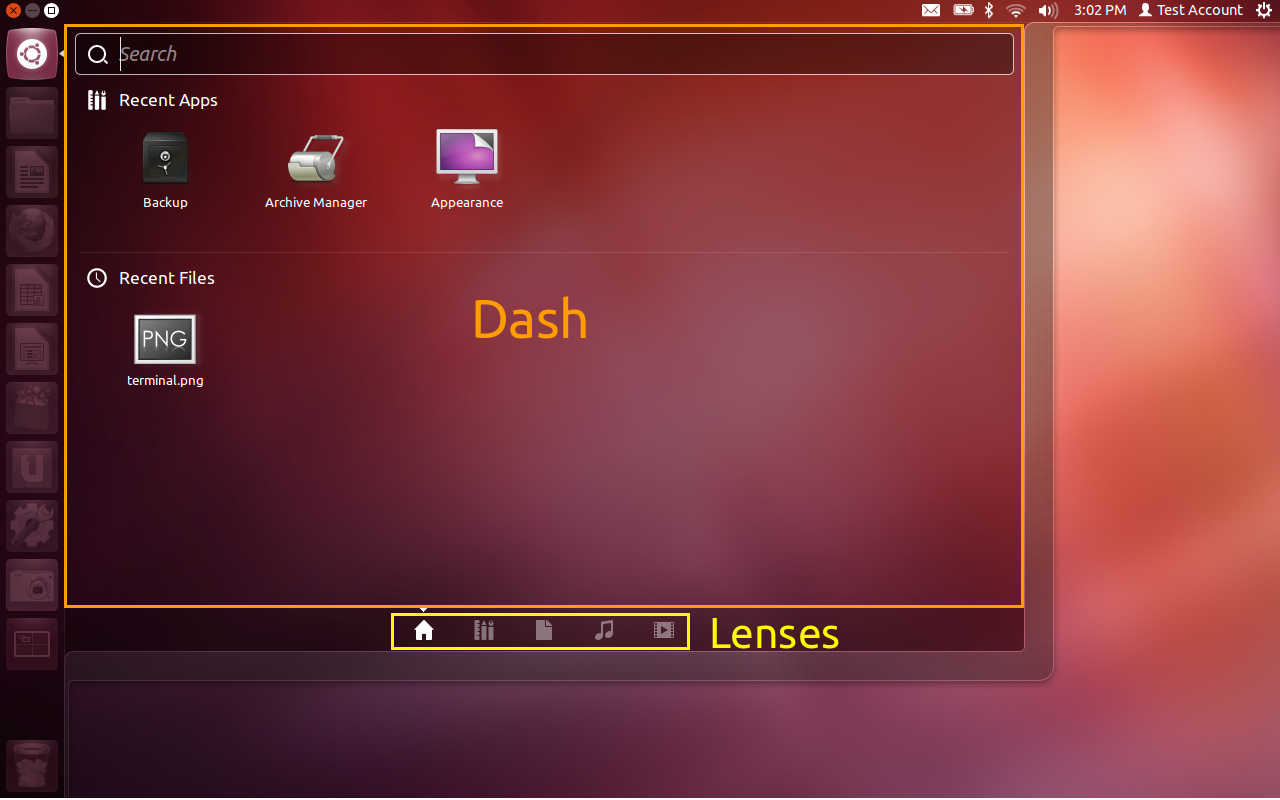
\includegraphics[width=400pt]{./images/desktop/dash.png}
	\caption{Unity Dash}	
	\label{fig:unity-dash}	
\end{figure}

\par \noindent The dash functionality can be extended to look for other stuff such as the web, youtube videos, cooking recipes directly from your dash by adding more lenses. Lenses \& Scopes are covered in more detail in the next section.  \\

\par \noindent Applications can now be quickly launched by pressing the Super key, type the application name and press enter to launch the application. \\

\par \noindent \framebox[6.7in][l]{\parbox[l]{6.5in}{\textbf{Tip}: You can pin any application to the launcher by dragging the application from the dash to the launcher and then right-clicking the application and pressing ``Lock to Launcher". If the application is already running, then you need to right click on the application icon in the launcher and then click on "Lock to launcher".}}

%\fbox{Tip: Quickly launch applications}

\section{Lenses \& Scopes} \index{Unity!Lenses}
Lenses are filters to show you only a specific type of data. You can see the lenses in figure \ref{fig:unity-dash} indicated by a yellow box. The lens In order of appearance (from the left to the right) are Home Lens, Application Lens, Files and Folders Lens, Music Lens and Video Lens. If you navigate to a specific lens like for instance the Music Lens, only your music files are shown while similarly only applications are shown in the Application lens. \\

\par \noindent Scopes are the back-end of lens as they dictate the sources where the information is gathered from. For instance, the file scope searches your hard disk for files and folder and displays it through the Files and Folders lens. It was mentioned before that the dash functionality could be extended. Well, this can be done by adding more lens which lets you search for other information as well. Additional lens can be installed from the Ubuntu Software Center. More about installing lens and applications are covered in chapter \ref{chap:software_management}. \\

\par \noindent \framebox[6.7in][l]{\parbox[l]{6.5in}{\textbf{Tip}: You can use the dash to quickly search for files and folder by using the file and folders lens.}}

\section{Top Panel and Indicators} \index{Indicators}
The top panel is the dark panel which can be seen in the top-hand of the desktop. At the top-right-hand side you can see some icons. This is illustrated by an orange box as can be seen in figure \ref{fig:ubuntu-desktop1}. The indicator as the name suggests are menus which indicate the status of applications. In order of appearance (from the left to the right) the indicators are messaging menu, battery menu, bluetooth menu, network menu, sound menu, clock, user menu and finally the system menu as can be seen in figure \ref{fig:unity-indicators}.

\begin{figure}[h]	
	\centering
	
\includegraphics[width=200pt]{./images/desktop/indicators.png}
	\caption{Indicators}	
	\label{fig:unity-indicators}		
\end{figure}

\begin{description}
	\item [Messaging menu] Easily launch and receive incoming notifications from messaging applications including email, social networking, and Internet chat.	
	\item [Battery menu] Check your laptop battery's charging status. This menu is hidden by default if a battery isn't detected.	
	\item [Bluetooth menu] Send or receive files by Bluetooth. This menu is hidden by default if a supported Bluetooth device isn't detected.	
	\item [Network menu] Connect to wired, wireless, mobile, and VPN networks.	
	\item [Sound menu] Set the volume, configure sound settings, and control media players like Vlc, Spotify, Rhythmbox.	
	\item [Clock] Access the current time and date.	
	\item [User menu] Change your password, language settings or login picture. Quickly switch between user accounts without logging out.	
	\item [System menu] Access system settings. Lock screen, log out, suspend, restart or shutdown your computer.	
\end{description}

\par \noindent Applications like Spotify and Rhythmbox (default Ubuntu music player) integrate into the sound menu. They automatically run in the background when you close them. You can control them directly from the sound menu without having to actually open that application. This can be seen in figure \ref{fig:sound-menu}. 

\begin{figure}[h]	
		\centering		
		\subfloat[Sound Menu]
		{ 	\label{fig:sound-menu} 	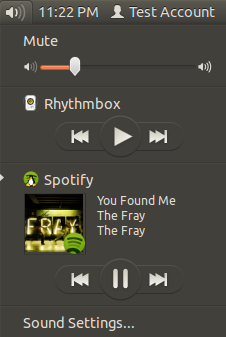
\includegraphics[width=100pt]{./images/desktop/sound-menu.png} } 
		~ \hspace{1in}
		\subfloat[Messaging Menu]
		{ 	\label{fig:messaging-menu} 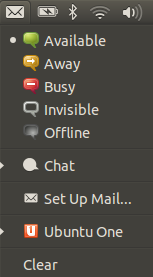
\includegraphics[width=90pt]{./images/desktop/messaging-menu.png}	}		
		\caption{Indicator Menus}
		\label{fig:unity-indicator-menus}
\end{figure}

\par \noindent Another useful indicator menu is the messaging menu. This menu is related to the social and communication related applications. Chat applications such as Empathy, Pidgin are integrated in this menu. This means that you can set the status of your messenger directly from this menu. It also provides option to set up your mail, and notifies you when new mail arrive. The messaging menu can be seen in figure \ref{fig:messaging-menu}.

\section{Heads Up Display - HUD} \label{sect:desktop-hud} \index{Heads Up Display}
%Definitely needs a screenshot in this section.
The Heads Up Display (HUD) is an intelligent search based approach to finding and accessing menu items you need. HUD automatically prioritises items that you frequently for easy access. How is this useful? Imagine you are using a new application. You no longer need to remember where a specific menu item is by hunting for it through the menus. With HUD, you can quickly search the task you want to perform and HUD will automatically show you the menu item you were looking for.  You can invoke the HUD by pressing the Alt key.\\

\begin{figure}[h]	
	\begin{center}
	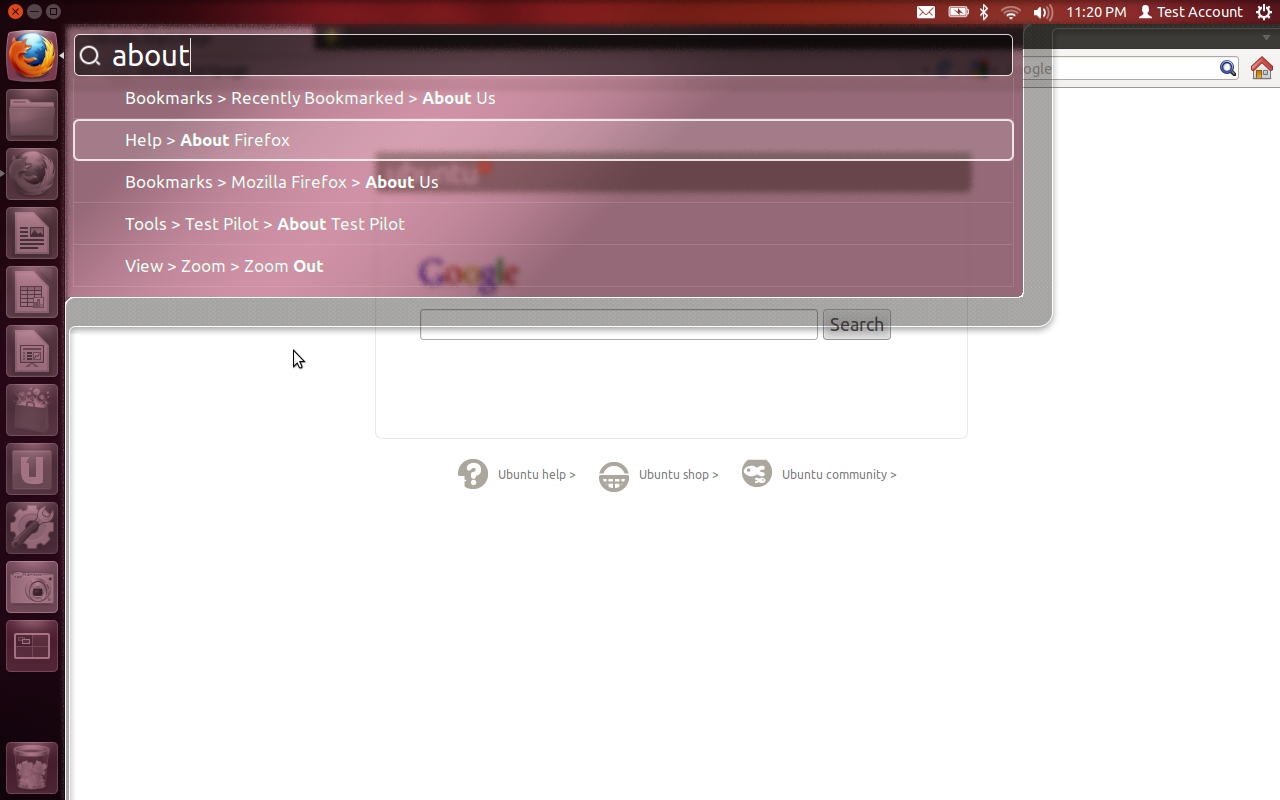
\includegraphics[width=400pt]{./images/desktop/HUD-firefox.png}
	\caption{Heads Up Display (HUD)}	
	\label{fig:unity-hud}	
	\end{center}
\end{figure}

\par \noindent For instance, let's assume a user using Firefox. If he want to customize his add-ons, he no longer needs to go through all the menus to find out where the add-ons menu item is present. He can using the HUD, search add-ons and HUD will present you with the menu item to customize add-ons. This is just one such instance, imagine how handy it woud be in applications with a lot of menus like Gimp or Blender.





\chapter{Software management} \label{chap:software_management}
In chapter \ref{chap:unity}, the basic usage of Ubuntu was briefly touched upon. In this chapter, let's continue this trend and learn about how to install applications  in Ubuntu. Managing applications in Ubuntu is slightly different from its counterpart operating systems such as Windows and Mac OS. By the end of this chapter you will have know to how to install software, update and upgrade your system. In order to make this easy to grasp, where ever possible a reference or similarity to other operating systems will be mentioned.

\section{Ubuntu Software Center} \index{Ubuntu Software Center}
Contrary to installing applications in the Windows operating system where you need to scour the internet to find common applications like Firefox, Thunderbird or any other 3rd party application, in Ubuntu this can all be done right from your desktop using the Ubuntu Software Center which can be seen in figure \ref{fig:usc}. 

\begin{figure}[h!]	
	\centering
	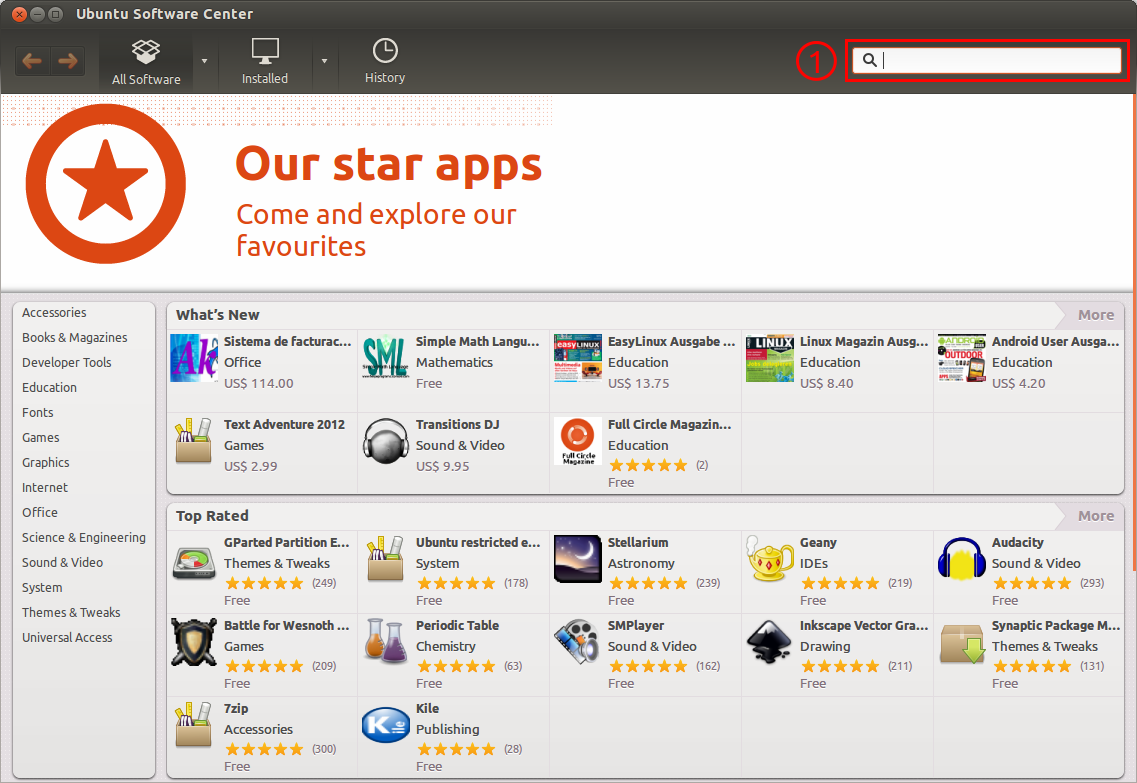
\includegraphics[width=325pt]{./images/applications/USC.png}
	\caption{Ubuntu Software Center}	
	\label{fig:usc}		
\end{figure}

\par \noindent You can launch the Ubuntu Software Center by pressing the Ubuntu Software Center icon in the launcher which looks like figure \ref{fig:usc-icon}. Or you can also launch Ubuntu Software Center from the dash as shown in section \ref{sect:dash}. 

\begin{figure}[h!]	
	\centering
	
\includegraphics[width=30pt]{./images/applications/usc-icon.png}
	\caption{Ubuntu Software Center launcher icon}	
	\label{fig:usc-icon}		
\end{figure}


\par \noindent The Ubuntu Software Center is a catalogue of applications, popular magazines and lenses. The Ubuntu Software Center is constantly being updated with new applications and content. If you are interested, you could yourself make an application which you submit for inclusion in the Ubuntu Software Center. It has a huge collection of applications produced by the community for the community. As can be seen in figure \ref{fig:usc}, the software center shows the top rated applications and also what's new. You can view applications by categories by clicking on one of the categories shown on the left. Try to explore the Ubuntu Software Center to get acquainted to the interface. It is a powerful application which can make managing application in Ubuntu much easier.\\

\section{Installing Application (via Ubuntu Software Center)} \label{sect:install-via-usc}

Let's try to install the program vlc using the software center.  You can do this by manually searching for vlc through the ``Sound and Video" category. However, a much quicker way is to search for vlc in the search box which can be in the top right of the software center (marked by a red box). On searching for vlc, you are presented with the search results as can be seen in figure \ref{fig:vlc-search}. 

\begin{figure}[h!]	
	\centering
	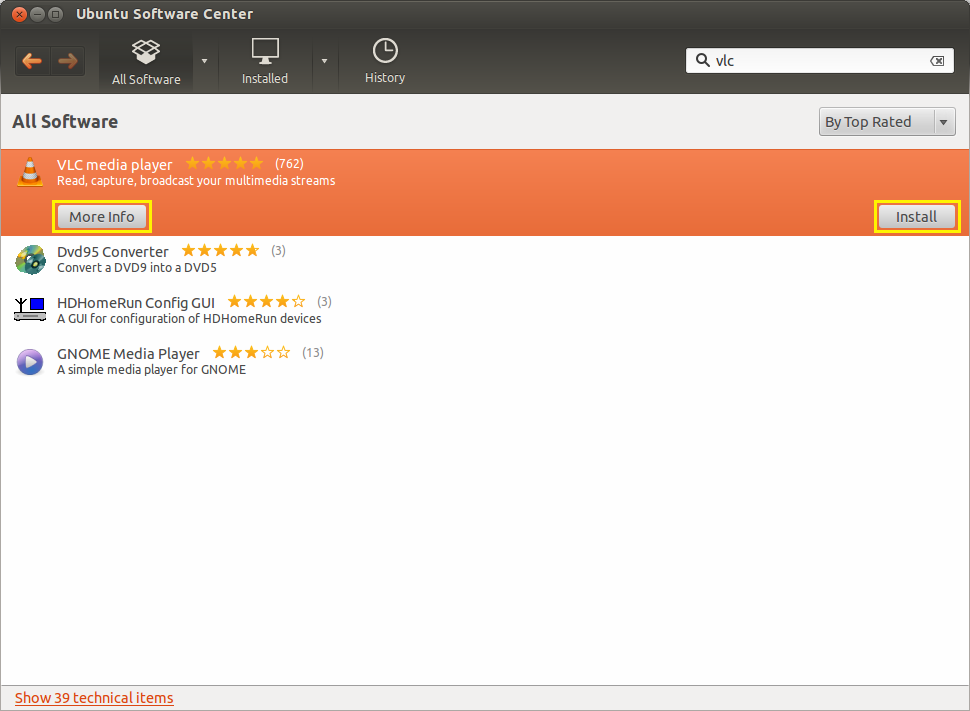
\includegraphics[width=300pt]{./images/applications/vlc-search.png}
	\caption{Search results}	
	\label{fig:vlc-search}		
\end{figure}

\par \noindent You can either install directly by pressing the install button. If you first wish to get more information about the application before you install, you can press more info. On pressing the more info button, you are presented with all the information about the application as seen in figure \ref{fig:vlc-info}. It shows the application description, the optional add-ons, reviews by other users and also other similar applications installed by other users.

\begin{figure}[h!]	
	\centering
	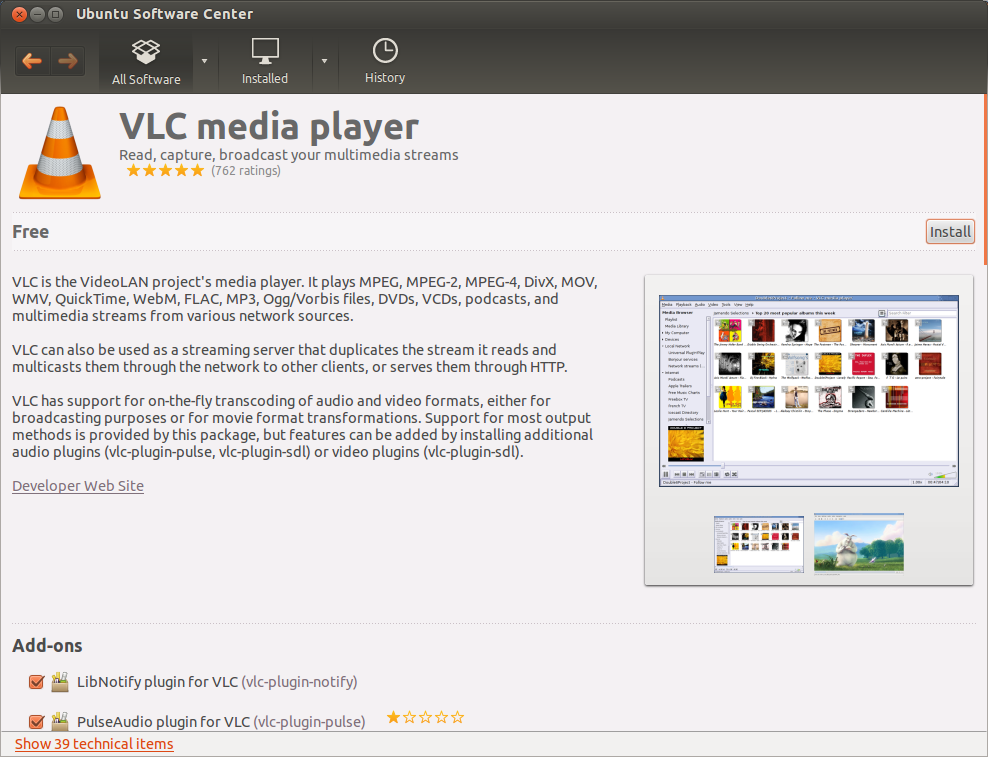
\includegraphics[width=300pt]{./images/applications/vlc-info.png}
	\caption{VLC application info}	
	\label{fig:vlc-info}		
\end{figure}

\par \noindent On pressing the install button, the installation starts in the background. You can either wait for it to install or you can do any other tasks that you wish to perform. You can keep a tab on the installation progress through the software center or in the launcher. This can be seen in figure \ref{fig:vlc-install}. \\

\begin{figure}[h!]	
	\centering
	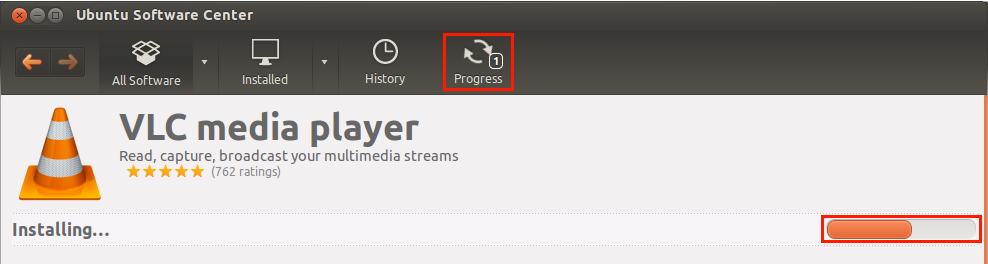
\includegraphics[width=325pt]{./images/applications/vlc-install.png}
	\caption{Installing vlc application}	
	\label{fig:vlc-install}		
\end{figure}

\par \noindent \framebox[6.7in][l]{\parbox[l]{6.5in}{\textbf{Tip}: You can install multiple applications at the same time without having to wait for one installation to complete to start another one. You can keep queuing applications you want to install. Ubuntu Software Center will automatically install all the queued applications one by one. }} \\

\section{Uninstalling Applications (via Ubuntu Software Center)}
As you saw in section \ref{sect:install-via-usc}, the installation process was a very simple task when done using the Ubuntu Software Center. Let's now see how to uninstall an application using the Ubuntu Software Center. The same application vlc will be used for this purpose. 

\begin{figure}[h!]	
	\centering
	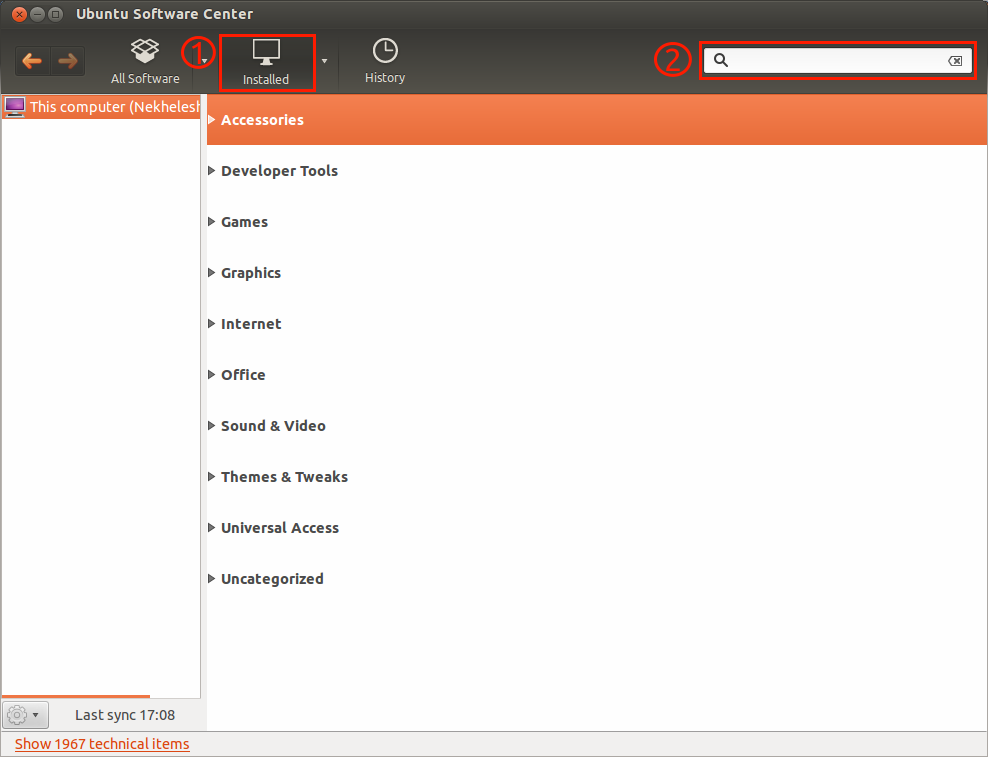
\includegraphics[width=325pt]{./images/applications/uninstall-apps.png}
	\caption{Uninstalling applications}	
	\label{fig:uninstall-apps}		
\end{figure}

\par \noindent First, you need to pressed the Installed button (marked with number 1) as can be seen in figure \ref{fig:uninstall-apps}. You are presented with the the different categories as seen in figure \ref{fig:uninstall-apps}. You can either search for vlc manually through the categories or you can search for vlc from search bar (marked by number 2) in figure \ref{fig:uninstall-apps}. When you search for vlc, the search results present vlc where you can uninstall by the clicking the button remove. This can be seen in figure \ref{fig:uninstall-vlc}.

\begin{figure}[h!]	
	\centering
	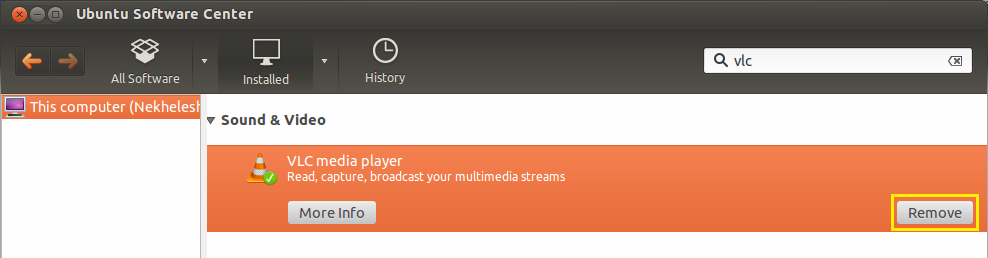
\includegraphics[width=325pt]{./images/applications/uninstall-vlc.png}
	\caption{Uninstalling vlc}	
	\label{fig:uninstall-vlc}		
\end{figure}

\section{Installation Applications (via other sources)}
Before proceeding further, it is important to explain a little bit about the application file type. In Windows, applications are distributed using executable files (.exe), while in Mac OS, you are given disk images (.dmg). In Ubuntu, applications are distributed in debian format (.deb). Remember this since you would be requiring this in the later part of this section. In the previous section, you were shown how to install applications using the Ubuntu Software Center. However, you are not constrained to installing application found in the Ubuntu Software Center. If you are unable to find your favourite application in the Ubuntu Software Center you can install that application using two other methods. \\

\par \noindent \framebox[6.7in][l]{\parbox[l]{6.5in}{\color{red} \textbf{Warning}: The installation methods described in this section allow the user to install other software, however please do not that installing software from random installation files (.deb) and Personal Package Package (PPA) found in the internet is not safe. They are not screened for security or stability. Use them with caution. All the softwares found in the Ubuntu Software Center has been carefully reviewed for these issues and is the best way to install applications in a secure manner.}} \\

\subsection*{Installation Files (.deb)} \index{deb}

The first method involves debian files (.deb). Let's illustrate this using an application such as Google Chrome. If you wanted to install Google Chrome, you can proceed to the Google's download page  \href{https://www.google.com/chrome}{\textit{here}}. Click download Google Chrome. You are then prompted with a dialog box asking which file you want to download as can be seen in figure \ref{fig:chrome-download}. Here you choose the 32-bit or 64-bit debian (.deb) file. This is marked by a red box in the figure.

\begin{figure}[h!]	
	\centering
	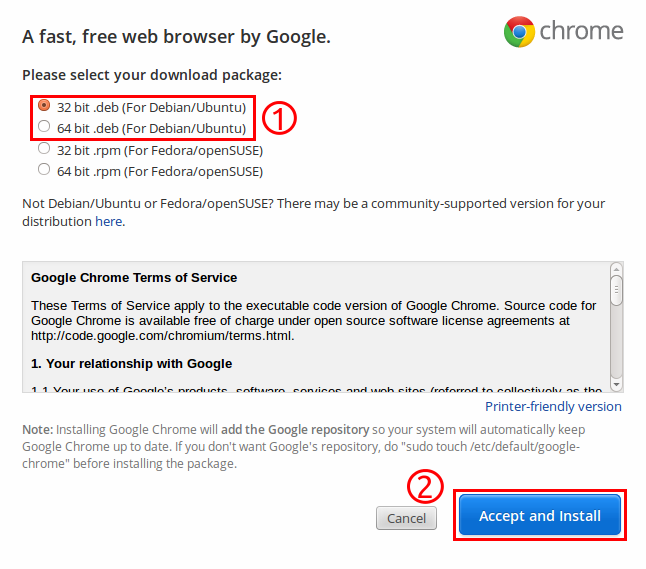
\includegraphics[width=300pt]{./images/applications/chrome-download.png}
	\caption{Download Google Chrome}	
	\label{fig:chrome-download}		
\end{figure}

\par \noindent Once it is downloaded to your system, you can find it in your Download folder by default. When you double click the installation file (.deb) as seen in figure \ref{fig:debfile-icon}, it is opened in the Ubuntu Software Center where you proceed to install it similar to the methods described in the previous sections. This disadvantage of installing applicating using .deb files is that these applications can only be updated manually and will not be done automatically using the update manager. \\

\begin{figure}[h!]	
	\centering
	\includegraphics[width=60pt]{./images/applications/debfile-icon.png}
	\caption{Google Chrome Installation file (.deb)}	
	\label{fig:debfile-icon}		
\end{figure}

\par \noindent \framebox[6.7in][l]{\parbox[l]{6.5in}{\textbf{Note}: The Google Chrome .deb installation file is an exception to updates. The .deb file installs Google Chrome in your system and also configures a Personal Package Archive (PPA). This way Google Chrome is automatically updated when new versions are available due to the PPA. This is explained in more detail below.}} \\

\subsection*{Personal Package Archives (PPA)} \index{Personal Package Archive}

The second method to install applications is using Personal Package Archives (PPA). A Personal Package Archive can be thought of a personal database of applications. As long as you are connected to this database (PPA), you get updates and softwares whenever the database is updated. Let's take the example of Google Chrome explained before. Google has its own PPA or database where it keeps the latest version of Google Chrome. So when Google Chrome is installed on your system, it also connects your system to the PPA. This way if the PPA is updated with a new version of Google Chrome, you automatically receive it as an update thereby ensuring automation to keep the software up to date. \\ 

\par \noindent Most of the times it is necessary to manually connect your system to a PPA. This can be done by following the directions given below. Launch the Ubuntu Software Center from the dash or the launcher. In the software center, open the edit menu and click Software Sources. This is shown in figure \ref{fig:software-sources-menu}.

\begin{figure}[h!]	
	\centering
	\includegraphics[width=350pt]{./images/applications/software-sources-menu.png}
	\caption{Software Sources Option}	
	\label{fig:software-sources-menu}		
\end{figure}

\par \noindent You are then presented with the software sources dialog as seen in figure \ref{fig:software-source}. Click on the Other Software tab.  \\

\begin{figure}[h!]	
	\centering
	\includegraphics[width=300pt]{./images/applications/software-source.png}
	\caption{Software Sources Dialog}	
	\label{fig:software-source}		
\end{figure}

\par \noindent In the Other Software tab, you can see all the current PPA which are present in your system. In figure \ref{fig:software-source-ppa}, you can see the four launchpad PPA installed on this system.  \\

\begin{figure}[h!]	
	\centering
	\includegraphics[width=300pt]{./images/applications/software-source-ppa.png}
	\caption{Software Sources - Other Software Tab}	
	\label{fig:software-source-ppa}		
\end{figure}

\par \noindent Click the Add button to add a PPA. In the Add PPA pop up dialog box as seen in figure x.xx, add the url to the PPA you want to install and click ok. You have now successfully added a PPA to your system. You need to now update the system manually using the update manager. You can launch the update manager from the dash. Click the check button in the update manager to check for updates manually. This is to inform the system about the newly added PPA. \\

\begin{figure}[h!]	
	\centering
	\includegraphics[width=300pt]{./images/applications/software-source-ppa-add.png}
	\caption{Software Sources - Add PPA}	
	\label{fig:software-source-ppa-add}		
\end{figure}

\par \noindent You can then install applications offered by the PPA directly from the software center. This is shown in figure \ref{fig:software-source-ppa-installapp}. In the figure \ref{fig:software-source-ppa-installapp}, you can see several PPA listed such as Polly Unstable PPA, Scopes Packagers Build, Tribler, Google etc. On selecting the PPA, you are then shown the list of application offered by that PPA. You can then proceed to install it similar to any other application.\\

\begin{figure}[h!]	
	\centering
	\includegraphics[width=350pt]{./images/applications/software-source-ppa-installapp.png}
	\caption{Software Sources - Install from PPA}	
	\label{fig:software-source-ppa-installapp}		
\end{figure}

\par \noindent \framebox[6.7in][l]{\parbox[l]{6.5in}{\textbf{Note}: Sometimes you might not see the PPA you recently added. This could be due to the software center not being refreshed yet. You can resolve this by restarting the software center or the system.}} \\

\section{Updates and Upgrades} \index{Updates} \index{Upgrades}
Just like other operating systems, it is important to update your Ubuntu system to ensure that your system is up to date and secure. Ubuntu will automatically prompt you for updates every week. The update manager will pop up showing the updates to all your software. The update manager can be seen in figure \ref{fig:update-manager}. If you want to check updates manually, you can do so by launching the update manager from the dash. There is however one important difference regarding updating in Ubuntu and other operating system. In Ubuntu, the update manager will show updates for all the applications installed in your system. This also includes the applications that you installed using the Ubuntu Software Center and using a Personal Package Archive (PPA). This is contrary to Windows, where the update manager only updates Windows and other Windows applications such as Microsoft Office etc. This way you do not need to worry about your installed applications being up to date. \\

\begin{figure}[h!]	
	\centering
	\includegraphics[width=325pt]{./images/applications/update-manager.png}
	\caption{Update manager}	
	\label{fig:update-manager}		
\end{figure}

\par \noindent It was explained in section \ref{chap:about_ubuntu_release} about new Ubuntu version released every 6 months while a new Long Term Support (LTS) is released every 2 years thought it is supported for 5 years on the desktop. You can choose to stick to the normal releases or stay with the LTS releases. You can change this setting by clicking on the settings button in the update manager as can be seen in figure \ref{fig:update-manager}. On clicking the button, you are presented with the settings dialog as can be seen in figure \ref{fig:update-preferences}. In the notify me of a new Ubuntu version, you can choose to be notified for new long term releases or for new normal releases. You will then be automatically prompted whenever a new version of Ubuntu is available. \\

\begin{figure}[h!]	
	\centering
	\includegraphics[width=325pt]{./images/applications/update-preferences.png}
	\caption{Update preferences}	
	\label{fig:update-preferences}		
\end{figure}

\par \noindent In the same settings dialog as seen in figure \ref{fig:update-preferences}, you can also set the frequency of the updates. By default, Ubuntu notifies of updates every week. You can change this to be displayed immediately or every two weeks.

\chapter{Terminal basics} \label{chap:terminal}
% Terminal Basics - cover important commands such as sudo, apt-get etc.
In chapter \ref{chap:unity}  you have read about Ubuntu's graphical user interface (GUI), Unity. You have also seen how to install/uninstall new software, update software repositories and upgrade the system. The latter is is connected with chapter \ref{chap:software_management} because some of them will be shown here too. Basically, you are shown two ways to perform the same task. Which method you chose depends on what you like best. \\

\par \noindent In a terminal you can do anything and everything than can done through a GUI. It varies from the most bast tasks such as  creating/removing directories and files, moving/copying  directories and files to advanced things like configuring your local area network (LAN), send mails and connect to remote server. \\

\par \noindent In this manual only the basics will be shown. Before you go any further please open a terminal. To open the terminal, click  on the Dash button and just search for terminal as shown in figure \ref{fig:open-terminal}. 

\begin{figure}[h]	
	\centering
	\includegraphics[width=400pt]{./images/terminal/open-terminal.png}
	\caption{Open terminal using dash}	
	\label{fig:open-terminal}	
\end{figure}

\par \noindent After that, you just left click on a terminal and wait for it to open. If you have done everything right, you should see the terminal window as shown in figure \ref{fig:terminal-window}.  \\

\begin{figure}[h]	
	\centering
	\includegraphics[width=300pt]{./images/terminal/terminal-window.png}
	\caption{Terminal Window}	
	\label{fig:terminal-window}	
\end{figure}

\par \noindent \framebox[6.7in][l]{\parbox[l]{6.5in}{\textbf{Note}: Examples from this point forward are  done in Ubuntu Lucid Lynx 10.04. Reason for that is due to Precise Pangolin being a test version while this tutorial is written.  (You will have Precise Pangolin labels if you installed it). Everything is same considering terminal and commands though. Prior pictures are taken under USB live running Precise Pangolin.}} \\ \\

\par \noindent With the terminal open, you can see a line of text.  What does this line of text indicate? First part of the text is your username. Also it states your /home partition. Second part of the text is your computer's name. This text also indicates which directory you are currently on. You can also check the current directory you are in by executing the \textit{pwd} command. For example,if the text is similar as shown in figure \ref{fig:pwd-command}, it means that you are now at home, to be more precise /home partition. \\

\begin{figure}[h]	
	\centering
	\fbox{\includegraphics[width=350pt]{./images/terminal/pwd-command.png}}
	\caption{pwd command}	
	\label{fig:pwd-command}	
\end{figure}

\par \noindent You can check that you are in a /home partition by just typing \textit{ls} command and pressing Enter. If you have done everything right you should see all files and folders that are under your /home partition. That is your data. See figure \ref{fig:ls-command} \\

\begin{figure}[h]	
	\centering
	\fbox{\includegraphics[width=350pt]{./images/terminal/ls-command.png}}
	\caption{ls command}	
	\label{fig:ls-command}	
\end{figure}

\par \noindent The command \textit{ls} lists all the files and folders in the directory you are currently on. Once the files and folders are shown, the terminal is waiting for you to type another command. This was basically just a small introduction to the terminal basics. Before learning about other commands, it is first essential to know about the different type of users to better understand the need for the commands covered later. \\

\par \noindent In chapter \ref{chap:about_ubuntu_why},  you read about Ubuntu's multi-user environment feature. You can be either an administrator or just a standard user. As an administrator you have more privileges than a standard user. On install by default you are provided with an administrator account meaning you have all the privileges unlike other people to whom you give  your computer for usage. \\

\par \noindent Let's proceed to the more important commands that are worth mentioning.

\section{SUDO command} \index{Sudo} \index{Terminal!Sudo}
% SUDO command - Describe
Commands such as \textit{ls}, are commands that every user can execute. In this chapter, commands that only the administrator of a computer can execute will be shown. \\

\par \noindent Sudo stands for  super user do (something that only an administrator can execute or do). This is not a command by itself but is rather used in combination with other commands that require administrative privileges. By using the sudo command, you are instructing the computer to run a command as an administrator. For example, let's try to update the system without sudo command. Type \textit{apt-get update} in the terminal and press Enter. After you have done that you should see something like shown in figure \ref{fig:sudo1}. \\

\begin{figure}[h!]	
	\centering
	\fbox{\includegraphics[width=350pt]{./images/terminal/sudo1.png}}
	\caption{apt-get update without sudo command}	
	\label{fig:sudo1}	
\end{figure}

\par \noindent If you got an error, that is a good sign. This just shows you that you cannot execute command apt-get update without the  sudo command in front of it. What the system does is to try to update the system as a regular user. Now, repeat the former step again but now type sudo in front of it  \textit{sudo apt-get update} and press Enter. You should be prompted with the administrator's password request. Type your password and press enter.  See figure \ref{fig:sudo2}.\\

\begin{figure}[h!]	
	\centering
	\fbox{\includegraphics[width=350pt]{./images/terminal/sudo2.png}}
	\caption{sudo apt-get update}	
	\label{fig:sudo2}	
\end{figure}

\par \noindent Do not worry if you don't see what you are typing. It is invisible but you are typing it though (invisibility is for security reasons). After you have finished just press Enter. You should see something like shown in figure \ref{fig:sudo3}. (The computer is updating its database of the latest software available for your computer.). \\

\begin{figure}[h!]	
	\centering
	\fbox{\includegraphics[width=350pt]{./images/terminal/sudo3.png}}
	\caption{Updating system's software database}	
	\label{fig:sudo3}	
\end{figure}

\par \noindent By now you should understand how the sudo command works. Later on there will be more examples showing the usage of the sudo command. \\

\par \noindent Note: Once you have entered  your password after sudo [-command-], the administrative mode is available for few minutes. This means that you can run other sudo [-command-] without entering the password. This mode becomes unavailable after a few minutes or after you close the terminal. \\

\section{Creating/Removing directories and files} \index{Terminal!Create/Remove} 
You probably know how to create folder or directory and file through the GUI. Here you will do those things via a terminal. The command to create a directory is mkdir. \\

\par \noindent \framebox[6.7in][l]{\parbox[l]{6.5in}{\textbf{Note}: If you give your directory a name via the terminal that has two or more words namely My pictures, you will have to connect those words with an underscore (\_). If you don't connect them with an underscore then the command will create two directories called My and pictures.}} \\

\par \noindent  Enter the command mkdir to create a folder in the terminal. This is illustrated in figure \ref{fig:mkdir1}.

\begin{figure}[h!]	
	\centering
	\fbox{\includegraphics[width=350pt]{./images/terminal/mkdir1.png}}
	\caption{Create a new directory}	
	\label{fig:mkdir1}	
\end{figure}

\par \noindent If nothing happens and you are prompted with your address again then everything is all right. To check that you have created folder type ls command and scroll down a bit to see if it is there. 

\begin{figure}[h!]	
	\centering
	\fbox{\includegraphics[width=350pt]{./images/terminal/mkdir2.png}}
	\caption{Directory Text}	
	\label{fig:mkdir2}	
\end{figure}
 
\par \noindent You can also check it via the graphical user interface. Go to the home directory to see if it is there. Suddenly you have decided that  you don't need that directory anymore. You can delete it. But let's try to do this using the terminal. Open your terminal again and type \textit{sudo rmdir Text}. Command rmdir is used to remove files and directories.

\begin{figure}[h!]	
	\centering
	\fbox{\includegraphics[width=350pt]{./images/terminal/rmdir1.png}}
	\caption{Remove directory}	
	\label{fig:rmdir1}	
\end{figure}

\par \noindent You can check if you have removed it from home folder/partition like explained before ( either ls or the GUI). As a small exercise, create another directory named Text. You will put files that you will create shortly after this into this folder. Now, type the command \textit{cd Text} and press Enter.  Command \textit{cd} lets you to navigate directories. In this case, you navigated into the Text directory. If you have done the cd command right, you should see something as shown in  illustration \ref{fig:mkdir4}.\\

\begin{figure}[h!]	
	\centering
	\fbox{\includegraphics[width=350pt]{./images/terminal/mkdir4.png}}
	\caption{Create new directory called Ubuntu}	
	\label{fig:mkdir4}	
\end{figure}

\par \noindent To get out of the directory just type \textit{cd} and  press Enter and nothing else. You should be back to your home directory. Next is to learn how to create a file. You should already know how to create a file via some text editor like Word, Writer, notepad etc. Here you will also need an editor to create a file. Default editor that comes with terminal is called gedit. That tool is going to be used here for examples. \\

\par \noindent \framebox[6.7in][l]{\parbox[l]{6.5in}{\textbf{Note}: File names have the same rules as directory. If you have two or more words connect them with underscore (\_). Text files in gedit have .txt extension.}} \\

\par \noindent To create a file that will be automatically saved in some directory command should look like this: gedit  file\_name.txt. Navigate into the directory named Text you created before. Let's create a file named ubuntu\_releases.txt. type into the terminal as shown in the illustration... and press Enter. (gedit  ubuntu\_releases.txt) \\

\begin{figure}[h!]	
	\centering
	\fbox{\includegraphics[width=350pt]{./images/terminal/mkdir5.png}}
	\caption{Create file}	
	\label{fig:mkdir5}	
\end{figure}

\par \noindent Soon you will be prompted with gedit editor, (perhaps you will be prompted with request for writing an administrators password). \\

\begin{figure}[h!]	
	\centering
	\includegraphics[width=350pt]{./images/terminal/mkdir6.png}
	\caption{Create file - Gedit Window}	
	\label{fig:gedit}	
\end{figure}

\par \noindent You can type into that editor just like any other. Also you can save what you have written. Try to type some of the Ubuntu releases namely: Lucid Lynx, Precise Pangolin etc. To save just do what you used to do in other editors by pressing CTRL+S. After you are done close the editor by clicking on the x sign in the upper left corner.  \\

\par \noindent \framebox[6.7in][l]{\parbox[l]{6.5in}{\textbf{Note}:  The text file will be saved in the directory from where you started the gedit editor. If you where in Ubuntu directory as shown in illustration \ref{fig:mkdir5}, then you should find your file named ubuntu\_releases.txt under that directory.  Later on it will be shown how to move and copy a file from one directory to other. }} \\

\par \noindent Before proceeding to copying and moving files lets first learn how to delete a file. Open your terminal if it is closed and check where your ubuntu\_releases.txt file. Hint (\textit{ls} to list what files and folders  you have in some directory, then cd  $<directory\_name>$ to enter and exit some directory.  \\

\par \noindent Deleting a file is similar process like deleting a folder or a directory. The only difference is the command. For deleting a file you have to write: \textit{rm file\_name} and press Enter. If you found your file (if you followed this tutorial it should be in your home folder. Type rm ubuntu\_releases.txt and press enter. To convince yourself that you deleted a file type ls or through the file manager. 

\begin{figure}[h!]	
	\centering
	\fbox{\includegraphics[width=350pt]{./images/terminal/rm1.png}}
	\caption{Delete file}	
	\label{fig:rm1}	
\end{figure}

\section{Moving/Copying directories and files} \index{Terminal!Move/Copy}
In this section you will see how to copy directory/file, move directory/file and remove the entire directory with all files at once. \\

\par \noindent To copy a directory  you should use this syntax, \fbox{cp  -r  directory\_name1 directory\_name2} where, \\

\par \noindent directory\_name1: Directory that you want to copy \\
directory\_name2: Directory where you want to copy directory\_name1 \\
-r :  this flag enables you to copy entire directory. The cp command alone copies only files. \\

\par \noindent As an exercise, let's create a new directory and name it DIR1 (hint:  \textit{mkdir DIR1}). After that create another directory and name it DIR2. Now try to copy DIR1 into DIR2 by executing \textit{cp -r DIR1 DIR2}. If everything went all right, you should find copy of a DIR1 under DIR2 as shown in figure \ref{fig:cp1}. \\

\begin{figure}[h!]	
	\centering
	\fbox{\includegraphics[width=350pt]{./images/terminal/cp1.png}}
	\caption{Copy directory}	
	\label{fig:cp1}	
\end{figure}

\par \noindent \framebox[6.7in][l]{\parbox[l]{6.5in}{\textbf{Note}: Notice that in the examples above you were working in your home folder. When you will want to copy folders/files in some other destinations you will have to use slash  / . With slash you tell the path where you want to copy something. For example you create another directory under DIR2 named DIR3. You decide that you want to copy some files from home folder to DIR3. It would go like this: \textit{cp  file\_name  DIR2/DIR3}  + enter. }} \\

\par \noindent Sometimes too many copies of something is not good. You would like to instead move them. So for moving or cutting a directory or a file the command mv is used. The command mv can also be used to rename files and directories. You should use the following syntax, \\

\par \noindent \fbox{mv directory\_name1  directory\_name2} \\

\par \noindent directory\_name1: folder you want to move or cut \\
directory2\_name: destination folder \\

\par \noindent Try to move already created and copied DIR1 into DIR2.  To do that execute \textit{sudo mv DIR1 DIR2} and hit Enter. If everything went all right you should have only one DIR1 under DIR2 and nowhere else. Check that with already mentioned command \textit{ls}. See figure \ref{fig:mv1}.

\begin{figure}[h!]	
	\centering
	\fbox{\includegraphics[width=350pt]{./images/terminal/mv1.png}}
	\caption{Move directory}	
	\label{fig:mv1}	
\end{figure}

\par \noindent How do you copy or move a file? It is similar to copying or moving directories. The same commands cp and mv are used. However the syntax is slightly different. To copy a file the syntax is \fbox{sudo cp file name destination}. Create a new file named file1.txt (hint:  \textit{sudo gedit file1.txt}, save it and exit from gedit). To copy it into DIR2 execute \textit{sudo  cp  file1.txt  DIR2} and hit Enter. (Check if file is copied with commands cd and ls). See figure \ref{fig:cp2}.

\begin{figure}[h!]	
	\centering
	\fbox{\includegraphics[width=350pt]{./images/terminal/cp2.png}}
	\caption{Copy file}	
	\label{fig:cp2}	
\end{figure}

\par \noindent To move a file the syntax is \fbox{sudo mv file name destination}. The procedure is similar to copying. The only difference is the command. Execute \textit{sudo mv file1.txt DIR2} and press enter. \\

\par \noindent \framebox[6.7in][l]{\parbox[l]{6.5in}{\textbf{Note}: If you will be prompted with message that old file1.txt in DIR2 will be overwritten just type y and press enter. After that your file should be only under DIR2 directory. See figure \ref{fig:mv2}.}} \\

\begin{figure}[h!]	
	\centering
	\fbox{\includegraphics[width=350pt]{./images/terminal/mv2.png}}
	\caption{Move file}	
	\label{fig:mv2}	
\end{figure}

\par \noindent What if you decide that you don't need all these directories and files? Under GUI you would just delete it with one click. Here you will delete it with one command. How to delete one file and directory you know (hint: commands rm and rmdir). To remove directory and all its content syntax is \fbox{rm -R directory\_name}.  (-R flag helps you to remove entire directory together with its content) \\

\par \noindent Try removing DIR2 by typing: sudo rm -R DIR2 and press enter. If everything went alright, DIR2 doesn't exist in home folder anymore.  See figure \ref{fig:mv3}. To convince yourself, check via GUI or via ls in terminal.  \\

\begin{figure}[h!]	
	\centering
	\fbox{\includegraphics[width=350pt]{./images/terminal/mv3.png}}
	\caption{Remove directory with content}	
	\label{fig:mv3}	
\end{figure}

\section{Submitting bug reports} \label{sect:bugreport-terminal} \index{Bug} 
As described in section \ref{chap:about_ubuntu_contribute}, bug reports are managed in Launchpad. It is one central place where the Ubuntu developers manage the bug submitted by users and try to fix the issues. Submitting bug reports to Launchpad can be easily done via the terminal using one simple command. This is illustrated in this section. In order to submit bug reports, you need to know the name of the package you are reporting the bug against. Once you know the name of the package, type \fbox{ubuntu-bug package\_name} as shown in figure \ref{fig:bugreport1}

\begin{figure}[h!]	
	\centering
	\fbox{\includegraphics[width=350pt]{./images/terminal/bugreport1.png}}
	\caption{Submit bug report}	
	\label{fig:bugreport1}	
\end{figure}

\par \noindent When you execute this command in the terminal, Ubuntu will collect all necessary information about your system automatically and create a bug report in Launchpad. You are however required to enter a bug title, description on how to reproduce this and provide any screenshots if necessary. A well described bug report will help the developers identify the problem quickly and solve the issue. It will then be issued as an update to all the Ubuntu users. \\

\par \noindent Some common package names are mentioned here. If it is graphical issue the most probable package is \emph{compiz}. So then you would type \emph{ubuntu-bug compiz}. If the bug is related to the dash or launcher, the package name is \emph{unity}. If you are unable to find the package name, just use of the above mentioned package names. The bug triagers will relate it to the correct package for you.

\newpage
\section{Installing/Uninstalling packages} \index{Terminal!Update/Upgrade packages}
You have already  seen how to install/uninstall packages via the Ubuntu Software Center. This section will show how to do this using the terminal. The command used for everything related to packages is called apt-get. For installing/uninstalling/removing software to be possible via the terminal, every distribution including Ubuntu has a ``package system that uses a private package database to keep track of which packages are installed, which are not installed and which are available for installation on your system. Considering installation, the apt-get command uses this database to find out how to install packages requested by the user and to find out which additional packages are needed in order for a selected package to work properly." \\

\par \noindent This section will cover the following topics,

\begin{itemize}
	\item update software repositories (mentioned database)
	\item upgrade system with new packages
	\item install/uninstall applications
	\item remove packages that are not needed any more
\end{itemize}

\par \noindent These are basic things and it is good to know them. This is just a start. You have to be aware that not everything can be configured or installed via GUI. Eventually you will have to step into terminal. It is similar to a car. You eventually will have to open the hood and check for the engine and the rest of the parts. The terminal also provides a way to perform task quickly without much delay.\\

\par \noindent Updating the package database is important so you can install newer versions of a software.  Without updating the database you could find yourself with errors like: some packages could not be installed or reached, invalid address etc. First part, updating a system's database you need to execute \textit{sudo apt-get update},  please see illustrations 7.8. and 7.9. \\

\par \noindent For upgrading the system's database with new packages you have to execute the command \textit{sudo apt-get dist-upgrade}.  If you wrote command correctly you should see something like illustration (number required).  You will be also prompted with question do you want to install update packages (for yes press y+enter, and for no press n+enter) as can be in figure \ref{fig:dist-upgrade}. \\

\begin{figure}[h!]	
	\centering
	\fbox{\includegraphics[width=350pt]{./images/terminal/dist-upgrade.png}}
	\caption{Upgrading system with new packages}	
	\label{fig:dist-upgrade}	
\end{figure}

\par \noindent Regular updating and upgrading your system's database helps you not just stay up-to-date as already mentioned but it helps your system to work properly. As you could have seen during an upgrade,  you didn't choose which packages to install, apt-get did it automatically for you. You just had to press y or n (yes or no). \\

\par \noindent You can also install package or a program individually by yourself. You saw how it is done via Ubuntu Software Center. With just one click you installed some applications. Here you will learn to install an application using just one command. You have to be careful that you don't fill your system with all kinds untrustworthy applications. That can cause you problems. Be careful what applications you install and from what source. It is recommended that you install what is in Ubuntu's database (better known repository). The easiest way to check that, is to visit Ubuntu's software center and type the name of an application. If it's not found there than you are installing an application at your own risk. \\

\par \noindent For installing an application  you have to execute \textit{sudo apt-get install $<application\_name>$ }\\

\par \noindent As simple as this is, you could hit a potential road block. You have to know what is the right name of a package or application so that you could install it. The Internet helps a lot in these situations. So don't worry. First is to try writing the application's name with lower case letters. For example if you don't have Skype installed on your system. Try executing \textit{sudo apt-get install skype}. If everything went all right you should see something like figure \ref{fig:install-skype}. \\

\begin{figure}[h!]	
	\centering
	\fbox{\includegraphics[width=350pt]{./images/terminal/install-skype.png}}
	\caption{Installing Skype}	
	\label{fig:install-skype}	
\end{figure}

\par \noindent After the installation is complete, you should see skype under your GUI (Ubuntu Software Center/Installed applications). 
If you decide to remove Skype, execute \textit{sudo apt-get remove skype} and press enter. The procedure is basically the same as with installation but is the other way around. Also, procedure is basically the same with other applications, \textit{ sudo apt-get remove <application\_name>} If you  typed command properly you should see something like figure \ref{fig:uninstall-skype}. \\

\begin{figure}[h!]	
	\centering
	\fbox{\includegraphics[width=350pt]{./images/terminal/uninstall-skype.png}}
	\caption{Uninstalling Skype}	
	\label{fig:uninstall-skype}	
\end{figure}

\par \noindent While using your system you might want to clean up unwanted packages left by some applications that are taking place on your disk. These packages were used by your system till one point. As the system is upgraded it doesn't need old ones, instead uses the new ones. So the old ones can be deleted. To remove unwanted/not needed packages execute \textit{sudo apt-get autoremove} and press enter. See figure \ref{fig:Autoremove}. \\

\begin{figure}[h!]	
	\centering
	\fbox{\includegraphics[width=350pt]{./images/terminal/autoremove.png}}
	\caption{Autoremove command}	
	\label{fig:Autoremove}	
\end{figure}

\par \noindent Tip: you can also use commands clean and autoclean.  \\

\par \noindent Do not think that this is it. There is much more. That ``much more" you will find at the Ubuntu official help pages. This will be described in more detail at the end of this manual. For conclusion of this chapter, Terminal is a very strong tool. Lot of ``stuff" can be fixed and configured here. You can see everything from different perspective and learn much more how system ``breathes". You don't have to memorise all commands. You have help/man. Use it wisely. 


\chapter{Performing basic tasks}
\section{Microblogging} \index{Social Networking}
Before describing how to start microblogging, it is good to explain what ``microblogging" actually represents. ``Microblogging is  a web service that allows the subscriber to broadcast short messages to other subscribers of the service. Micropost can be made public on a web site  and/or distributed to a private group of subscribers. Subscribers can read microblog posts online or request updates to be delivered in real time to their desktop or a mobile device via SMS text message". The term web services in that context include Twitter, Facebook etc. \\

\par \noindent Ubuntu by default supports microblogging. This essential means that you can read facebook posts, twitter tweets directly from the Ubuntu desktop. Here it will be shown how to set up microblogging in Ubuntu. Application that will be used for this example is Gwibber. ``Gwibber is an open source microblogging client for Ubuntu. It brings the most popular social networking web services to your desktop and gives you the ability to control how you communicate". Gwibber is a pre-installed application on your Ubuntu system. You just have to go to the dash and type Gwibber. \\

\par \noindent Further in this chapter will be shown how to: 

\begin{itemize}
		\item Set up Gwibber for Twitter
		\item Test the Gwibber for Twitter to see how it works
\end{itemize}

\subsection*{Step 1.  Opening Gwibber application via Dash}

\par \noindent Open the dash and search for gwibber. \\

\begin{figure}[h!]	
	\centering
	\includegraphics[width=300pt]{./images/basic-tasks/gwibber1.png}
	\caption{Launch Gwibber from the dash}	
	\label{fig:gwibber1}		
\end{figure}

\subsection*{Step 2.  Short tour through Gwibber's interface}

\par \noindent After you left click Gwibber's icon on a dash you are prompted with Gwibber's dialog boxes. See figure \ref{fig:gwibber2}. \\

\begin{figure}[h!]	
	\centering
	\includegraphics[width=200pt]{./images/basic-tasks/gwibber2.png}
	\caption{Gwibber web services}	
	\label{fig:gwibber2}		
\end{figure}

\par \noindent As you can see in figure \ref{fig:gwibber2},  this dialog box serves you to set up microblogging for the already mentioned web services like Twitter, Facebook etc. You will see that later on more detailed. 

\subsection*{Step 3.  Setting up the Gwibber for Twitter}

In figure \ref{fig:gwibber2} choose Twitter.  After you have chosen Twitter just left click the Add button. Next step is to start the authorization process with Twitter. Gwibber and Twitter have to be synchronized. Twitter has to authorize your access via Gwibber. To start the authorization you have to left click on the button Authorize. \\

\begin{figure}[h!]	
	\centering
	\includegraphics[width=200pt]{./images/basic-tasks/gwibber3.png}
	\caption{Configure account}	
	\label{fig:gwibber3}		
\end{figure}

\par \noindent As shown on in figure \ref{fig:gwibber3}, you can also set up others features like: receiving/sending messages, account color. After you have done that just click on the button Authorize. Further more you will be prompted with dialog box where you will have to enter your Twitter login credentials. See figure \ref{fig:gwibber4}. After you have entered your Twitter username and password you have to left click on the button Authorize app. \\

\begin{figure}[h!]	
	\centering
	\includegraphics[width=200pt]{./images/basic-tasks/gwibber4.png}
	\caption{Twitter user credentials}	
	\label{fig:gwibber4}		
\end{figure}

\par \noindent You will have to wait until Twitter and Gwibber are synchronized. After synchronization is done you will be prompted that your account via Gwibber has been authorized. You can now close Gwibber's account setup dialog window.Now you can start messaging and looking at your tweet feed. (This will be shown on illustrations 8.1.10. to 8.1.12. \\

\par \noindent What you will see is:

\begin{itemize}
\item How does the interface looks like when you are reaching Twitter via Gwibber
\item How to send message via Gwibber
\item Tweet feed via Gwibber
\end{itemize}

\begin{figure}[ht!]	
		\centering		
		\subfloat[Gwibber Twitter interface]
		{ 	\label{fig:sound-menu} 	\includegraphics[width=200pt]{./images/basic-tasks/gwibber5.png} } 
		~ \hspace{0.5in}
		\subfloat[Gwibber Twitter tweet feed]
		{ 	\label{fig:messaging-menu} \includegraphics[width=200pt]{./images/basic-tasks/gwibber6.png}	}		
		\caption{Gwibber interface}
		\label{fig:gwibber}
\end{figure}


\section{Listening to music} \index{Music}
In Ubuntu, Rhythmbox is the default music player. You can launch the music player through the dash by searching for Rhythmbox. You also launch the music player using the sound menu. This is much quicker and easier to access at any time. This is illustrated in figure \ref{fig:play-music1}. The sound menu houses media applications and sound control settings. If you install other media applications such as Spotify, they will be automatically added to the sound menu. \\

\begin{figure}[h!]	
	\centering
	\includegraphics[width=150pt]{./images/basic-tasks/play-music1.png}
	\caption{Launch Rhythmbox from the sound menu}	
	\label{fig:play-music1}		
\end{figure}

\par \noindent The Rhythmbox music player can be seen in figure \ref{fig:play-music2}. It behaves like any standard media player. You can create playlists with your favourite music and save it for future playback. On first launch, Rhythmbox automatically starts importing all your music present in your music folder. You can also configure it to watch a specific folder for new music. Rhythmbox also includes the Ubuntu One music store where you can purchase music using your Ubuntu One account. If you do not have an account, you can create it easily. \\

\begin{figure}[h!]	
	\centering
	\includegraphics[width=250pt]{./images/basic-tasks/play-music2.png}
	\caption{Rhythmbox}	
	\label{fig:play-music2}		
\end{figure}

\par \noindent Since Rhythmbox can be easily accessed from the sound menu, you can also perform other operations from the sound menu directly. You can control all media operations such as Play, Pause, Forward, Reverse, choose playlist all within the sound menu without having to show the Rhythmbox interface. This allows for quick control of media playback. Imagine a scenario where you have several applications open. Instead of opening Rhythmbox and then controlling the music, you can just do this using the sound menu while Rhythmbox runs in the background. \\

\begin{figure}[h!]	
	\centering
	\includegraphics[width=150pt]{./images/basic-tasks/play-music3.png}
	\caption{Rhythmbox - Play/Pause}	
	\label{fig:play-music3}		
\end{figure}

\par \noindent \framebox[6.7in][l]{\parbox[l]{6.5in}{\textbf{Note}: When you click the close button, Rhythmbox does not quit but rather is still running in the background. This is intentional and intended to allow the user to continue with his work while the music player runs in the background. If you want to quit it, you have to choose quit from the Music menu.}} \\

\section{Editing Documents, Presentations, Spreadsheets} \label{sect:office}
Ubuntu by default comes with an office suite to help you get started straight away. You no longer need to worry about installing it after a fresh install of Ubuntu. LibreOffice is the office suite which is provided by default by Ubuntu. It is similar to Microsoft Office (Windows) or Office for Mac (Mac OS). Launching the office suite can be done by launching it from the dash or also from the launcher. LibreOffice Writer is similar to Microsoft Word, LibreOffice Calc is similar to Microsoft Excel and finally LibreOffice Impress is the counterpart of Microsoft Powerpoint. These programs are already present in your launcher and look like figure \ref{fig:office-icons}. \\

\begin{figure}[ht!]	
		\centering		
		\subfloat[]
		{ 	\label{fig:sound-menu} 	\includegraphics[width=40pt]{./images/basic-tasks/document-icon.png} } 
		~ \hspace{0.5in}
		\subfloat[]
		{ 	\label{fig:messaging-menu} \includegraphics[width=40pt]{./images/basic-tasks/spreadsheet-icon.png}	}
		~ \hspace{0.5in}
		\subfloat[]
		{ 	\label{fig:messaging-menu} \includegraphics[width=40pt]{./images/basic-tasks/presentation-icon.png}	}
		\caption{Libreoffice icons}
		\label{fig:office-icons}
\end{figure}

\par \noindent LibreOffice is backed up by many companies, to name some of the prominent ones are Google, Red Hat, Novell etc. LibreOffice can handle all the documents created by Microsoft Office, so rest assured you will not run into collaboration problems (However LibreOffice doesn't have 100\% accuracy at importing or exporting Microsoft Office formats.). Writer, Calc and Impress can be seen in figure \ref{fig:edit-office}.

\begin{figure}[h!]	
	\centering
	\includegraphics[width=300pt]{./images/basic-tasks/edit-office.png}
	\caption{Libreoffice}	
	\label{fig:edit-office}		
\end{figure}

\section{Setting up the internet} \index{Network}
Setting up the Internet under Ubuntu is pretty easy because everything works pretty much out of the box. You do not need to configure anything. The wireless networks detected are automatically shown in the networks menu in the top panel. The only think you are required to input are the password of the password protected networks. \\

\begin{figure}[h!]	
	\centering
	\includegraphics[width=150pt]{./images/basic-tasks/internet1.png}
	\caption{Network menu}	
	\label{fig:internet1}		
\end{figure}

\par \noindent However, sometimes you might want to edit your connections to change the settings. This can be done by clicking the Edit Connection menu items as seen in figure \ref{fig:internet2}.You will then be prompted with the Edit connection dialog window. See figure \ref{fig:internet3}. In the edit connections dialog window, you can configure the settings of any network profile that you wish to change. This includes all wired, wireless networks, mobile broadband, VPN and DSL. \\

\begin{figure}[ht!]	
		\centering		
		\subfloat[Edit Connections menu item]
		{ 	\label{fig:internet2} 	\includegraphics[width=150pt]{./images/basic-tasks/internet2.png} } 
		~ \hspace{0.5in}
		\subfloat[Edit Connections dialog window]
		{ 	\label{fig:internet3} \includegraphics[width=200pt]{./images/basic-tasks/internet3.png}	}		
		\caption{Edit Connections}
		\label{fig:internet23}
\end{figure}

\par \noindent To edit/configure wired connection you have to left click on Edit button as shown in figure \ref{fig:internet3} so you could proceed to the wired connection set up. See figure \ref{fig:internet4}. As you can see in figure \ref{fig:internet4}, you can, 

\begin{itemize}
	\item Give the network connection a name.
	\item Decide if you want to connect to this particular network automatically when available.
	\item Edit the device MAC address  - this is already done by the system automatically. Note: wired connection is always named eth0 and wireless wlan0 by the system. If you will ever configure connection via Terminal you will need these labels. 
	\item Edit cloned MAC address
	\item Edit MTU (Maximum transmission unit)
\end{itemize}

\par \noindent Note: Network icon on the bar will change into two arrows pointing in two different directions when connection to the Internet is established. See figure \ref{fig:internet6}. \\

\begin{figure}[ht!]	
		\centering		
		\subfloat[Edit Connections menu item]
		{ 	\label{fig:internet4} 	\includegraphics[width=200pt]{./images/basic-tasks/internet4.png} } 
		~ \hspace{0.5in}
		\subfloat[Wired connection complete]
		{ 	\label{fig:internet6} \includegraphics[width=150pt]{./images/basic-tasks/internet6.png}	}		
		\caption{Wired connection setup}
		\label{fig:internet46}
\end{figure}

\par \noindent Configuring wireless networks can be done in a similar fashion. You need to bring up the Edit connections dialog from the networks menu and then choose the wireless tab. Here you are shown the wireless networks you have previously connected to. The method is exactly similar to the wired approach described above and hence will not be repeated again. \\

\section{Printing documents, pictures} \index{Print}
You have read about the LibreOffice suit in section \ref{sect:office}. Printing documents in Ubuntu is very easy. Let's try printing a document using LibreOffice Writer. Open LibreOffice Writer and create a document. After that left click on the File menu and then click the Print submenu item. See figure \ref{fig:print1}. \\

\begin{figure}[h!]	
	\centering
	\includegraphics[width=300pt]{./images/basic-tasks/print1.png}
	\caption{Libreoffice Writer Print Menu}	
	\label{fig:print1}		
\end{figure}

\par \noindent Shortly you will be prompted with Print dialog window as seen in figure \ref{fig:print2}. \\

\begin{figure}[h!]	
	\centering
	\includegraphics[width=200pt]{./images/basic-tasks/print2.png}
	\caption{Print Dialog}	
	\label{fig:print2}		
\end{figure}

\par \noindent Note: Most of the printers today work by the principle ``plug and play"  (hint USB).  Well, on some operating systems like Windows you may have to install a driver for a printer that you buy. You do not need to do that for Ubuntu, at least not for EPSON printers. Ubuntu recognizes them automatically at once just like the wireless networks in previous sections. All you have to do is wait a bit when you plug your printer into the computer until they synchronize. After that you can print as shown in figure \ref{fig:print2}. Procedure for printing pictures is the same as for printing documents.

\section{Composing Emails} \index{Email}
Mozilla Thunderbird is the default email client of Ubuntu. It boasts features such as Migration assistant to help you migrate from other desktop email clients, mail account setup wizard, tabbed interface and many other features. You can find more information about thunderbird \href{http://www.mozilla.org/en-US/thunderbird/features/}{here}. This section will show how to set up your e-mail and send a message. You can start Thunderbird by clicking on the e-mail icon on the top panel (shape of an envelope).  After that you have to left click on the sub menu item called Set up mail. See figure \ref{fig:thunderbird1}. \\

\begin{figure}[h!]	
	\centering
	\includegraphics[width=150pt]{./images/basic-tasks/thunderbird1.png}
	\caption{Mozilla Thunderbird email client}	
	\label{fig:thunderbird1}		
\end{figure}

\par \noindent After that you will be prompted with Thunderbird's wizard for setting up an e-mail account. First step is to write your name,  e-mail address that you use and its password. (What ever you use: gmail, yahoo, hotmail etc.). See figure \ref{fig:thunderbird2}. Press Continue to proceed to the next step of the wizard.\\

\begin{figure}[h!]	
	\centering
	\includegraphics[width=200pt]{./images/basic-tasks/thunderbird2.png}
	\caption{Mail Account setup wizard}	
	\label{fig:thunderbird2}		
\end{figure}

\par \noindent Thunderbird will automatically set up the email account for you. Press the Create Account button on the wizard to complete the setup as seen in figure \ref{fig:thunderbird3}. After that you will have to wait for Thunderbird to synchronize all the emails and sets up you account. You no longer need to access your email from a web interface such as gmail.com or hotmail.com. You can access all your email right from your desktop. \\

\begin{figure}[h!]	
	\centering
	\includegraphics[width=200pt]{./images/basic-tasks/thunderbird3.png}
	\caption{Mail Account setup wizard}	
	\label{fig:thunderbird3}		
\end{figure}

\par \noindent You will then be prompted with Thunderbird's System Integration dialog box, where you will be asked for what you want to use Thunderbird by default. In this case it is just E-mail). See figure \ref{fig:thunderbird4}. Now you are ready to compose a new message. \\

\begin{figure}[h!]	
	\centering
	\includegraphics[width=200pt]{./images/basic-tasks/thunderbird4.png}
	\caption{System Integration dialog}	
	\label{fig:thunderbird4}		
\end{figure}

\par \noindent To compose a new message you have to click on a Write new message command as shown in figure \ref{fig:thunderbird5}. After that you will be prompted with a familiar interface for composing an email as seen in figure \ref{fig:thunderbird6}.

\begin{figure}[h!]	
	\centering
	\includegraphics[width=150pt]{./images/basic-tasks/thunderbird5.png}
	\caption{Create new message}	
	\label{fig:thunderbird5}		
\end{figure}

\begin{figure}[h!]	
	\centering
	\includegraphics[width=300pt]{./images/basic-tasks/thunderbird6.png}
	\caption{Compose new message}	
	\label{fig:thunderbird6}		
\end{figure}

\section{Browsing the web} \index{Browse}
Mozilla Firefox is the default web browser of Ubuntu. Firefox is an open source application which is cross-platform, meaning you can use it other operating systems such as Windows and Mac OS. It is the second most popular web browser in the world. You can launch Firefox either from the launcher or the dash. You can see the Firefox interface in figure \ref{fig:firefox2}. \\

\begin{figure}[h!]	
	\centering
	\includegraphics[width=300pt]{./images/basic-tasks/firefox2.png}
	\caption{Mozilla Firefox web browser}	
	\label{fig:firefox2}		
\end{figure}

\par \noindent Firefox supports tabbed browsing, synchronization with other devices and provides support to customize your browser using add-ons which can be downloaded from their website at \href{www.firefox.com}{firefox.com}. Updates to Firefox are automatically done by Ubuntu to ensure that you have the latest modern web browser on your system.

\newpage
\section{Sharing files with other users} \index{Ubuntu One} \index{Personal Cloud} \index{Web Storage}
Ubuntu 12.04 by default comes with the popular file sharing program called Ubuntu One. It is a personal storage space (cloud) on the web to store files, music and videos. Every Ubuntu user is entitled to an Ubuntu One account which by default offers 5 GB storage space. You are required to create a Ubuntu account which can also be used for other purposes like Launchpad, Ubuntu Software Center, Ubuntu Shop and other Ubuntu services. Ubuntu One offers the following features,

\begin{itemize}
	\item 5 GB free storage space on the web (cloud storage)
	\item Share and access your files from multiple devices like your computer, phones etc.
	\item Stream your music across all your portable devices.
	\item Available for many platforms
\end{itemize}

\par \noindent Ubuntu One is available on many platforms like Windows, Android, iPhone, iPad and also expected to arrive for the Mac OS at the time of writing this manual. This way you can share files without any hassle among these devices through Ubuntu One. Ubuntu One can be compared to other online file storage applications like iCloud, Dropbox etc. Ubuntu One also also provides music streaming feature. You can wirelessly sync your music to your portable devices to have music on the go. And since Ubuntu One is available for Android and iPhone, you have access to the entire music collection present on your computer at home.\\

\par \noindent Let's consider a scenario where you have multiple laptop running Windows operating system, Ubuntu and also other portable devices such as you Android phone. Ubuntu One allows you to share your files to all these devices. So instead of having to copy/paste files on to each of these devices individually, you can instead just save the file in your Ubuntu One web storage and these will automatically be available on all your devices. In this section, instructions to create an Ubuntu One account and share files with other users will be shown. 

\subsection*{Setting up Ubuntu One}

\par \noindent Click on the Ubuntu One application icon on the launcher. It looks like figure \ref{fig:share1}. This icon also displays the sync status once the configuration process is complete.

\begin{figure}[h!]	
	\centering
	\includegraphics[width=40pt]{./images/basic-tasks/share1.png}
	\caption{Ubuntu One application icon}	
	\label{fig:share1}		
\end{figure}

\par \noindent On clicking the icon for the very first time on a new Ubuntu install, you are presented with the Ubuntu One install wizard as shown in figure \ref{fig:share2}. Click the install button to start the installation. 

\begin{figure}[h!]	
	\centering
	\includegraphics[width=300pt]{./images/basic-tasks/share2.png}
	\caption{Ubuntu One install wizard}	
	\label{fig:share2}		
\end{figure}

\par \noindent Once the installation is complete, you are shown the setup wizard where the steps required to complete the initial Ubuntu One configuration is shown. Since the installation is complete, the remaining steps include signing in to your Ubuntu One account, choosing the folders to sync and then finally synchronisation itself. First, you can either choose to login into an existing account or create a new account. Both choices will be explained below. \\

\begin{figure}[h!]	
	\centering
	\includegraphics[width=300pt]{./images/basic-tasks/share3.png}
	\caption{Ubuntu One account setup}	
	\label{fig:share3}		
\end{figure}

\par \noindent Let's first start with signing in to an existing account. When you click on \textit{Sign me in with my existing account}, you are presented with a dialog window where you enter your Ubuntu One user credentials as shown in figure \ref{fig:share4}. Once you are done, click Sign In. \\

\begin{figure}[h!]	
	\centering
	\includegraphics[width=300pt]{./images/basic-tasks/share4.png}
	\caption{Ubuntu One user credentials}	
	\label{fig:share4}		
\end{figure}

\newpage
\par \noindent In this step, you can choose which folders you want to sync from the cloud (web storage) to your computer. This is useful to only sync the required files. For instance, on your mobile phone you might not want to sync all the files but rather just selected music files perhaps. Once done, click the Next button.\\

\begin{figure}[h!]	
	\centering
	\includegraphics[width=300pt]{./images/basic-tasks/share8.png}
	\caption{Syncing cloud to computer}	
	\label{fig:share8}		
\end{figure}

\par \noindent In the final step, you can choose which folders you want to sync from your device to the cloud storage. You might be interested to only sync important files to the cloud to save space. You can choose any folder that you want from your computer. Any changes that you make in that folder will be automatically synchronised to the cloud. Hence all your devices which are connected to Ubuntu One will always be up to date. \\

\begin{figure}[h!]	
	\centering
	\includegraphics[width=300pt]{./images/basic-tasks/share9.png}
	\caption{Syncing computer to cloud}	
	\label{fig:share9}		
\end{figure}

\newpage
\par \noindent Let's now return to the step where you have to create a new Ubuntu One account. If you clicked \textit{I don't have an account yet- sign me up} in figure \ref{fig:share3}, you are then presented with a form, where you can fill in all the required information to create a Ubuntu One account. This is easy to follow and the steps are pictorially represented below in figures \ref{fig:share5} and \ref{fig:share7}. \\

\begin{figure}[h!]	
	\centering
	\includegraphics[width=300pt]{./images/basic-tasks/share5.png}
	\caption{Enter user credentials}	
	\label{fig:share5}		
\end{figure}

\begin{figure}[h!]	
	\centering
	\includegraphics[width=300pt]{./images/basic-tasks/share7.png}
	\caption{Enter verification code}	
	\label{fig:share7}		
\end{figure}

\newpage
\par \noindent When all the steps are complete, you are finally shown the Ubuntu One control panel. This is the central place from where you can manage all your Ubuntu One settings. You can choose the download/upload speeds, personal details, choose which folders to sync etc. Try to spend some time getting acquainted with the Ubuntu One control panel. It will come handy in the future when you want to change some settings. You can see the Ubuntu One control panel in figure \ref{fig:share10}. \\

\begin{figure}[h!]	
	\centering
	\includegraphics[width=300pt]{./images/basic-tasks/share10.png}
	\caption{Ubuntu One control panel}	
	\label{fig:share10}		
\end{figure}

\par \noindent Now that Ubuntu One has been configured, let's see how to share files, understand file sync status and also publish files. The methods below can also be done using the web interface which can be accessed at \href{https://one.ubuntu.com/}{one.ubuntu.com}.

\subsection*{Sync Status and Publishing Files} \index{Ubuntu One!Publish Files}
Open the file manager and click on the Ubuntu One bookmark shown on the left column. In the Ubuntu One folder, you will find all the files which are synced to this device (computer, phone etc).  It important to see what icons are used to represent the sync status first. The files in the Ubuntu One will have these emblems on each file and folder icon to indicate their syncing status. 

\begin{figure}[ht!]	
		\centering		
		\subfloat[Updating]
		{ 	\label{fig:updating_emblem} 	\includegraphics[width=40pt]{./images/basic-tasks/updating_emblem.png} } 
		~ \hspace{0.5in}
		\subfloat[Synced]
		{ 	\label{fig:synced_emblem} \includegraphics[width=40pt]{./images/basic-tasks/synced_emblem.png}	}
		~ \hspace{0.5in}
		\subfloat[Unsynced]
		{ 	\label{fig:unsynced_emblem} \includegraphics[width=40pt]{./images/basic-tasks/unsynced_emblem.png}	}		
		\caption{Syncing Status}
		\label{fig:syncing_status}
\end{figure}

\par \noindent If you wanted to share a file to anyone on the internet, you can do so by using the publishing feature of Ubuntu One. When you publish a file, you are given a web link to the file. You can share this web link anywhere to anyone to access your file. To publish a file, right-click the file that you want to publish, under Ubuntu One, click publish as shown in figure \ref{fig:publish}. You are then provided with a web link which you can then use to let others see the file.  \\

\begin{figure}[h!]	
	\centering
	\includegraphics[width=300pt]{./images/basic-tasks/publish.png}
	\caption{Publish a file}	
	\label{fig:publish}		
\end{figure}

\par \noindent \framebox[6.7in][l]{\parbox[l]{6.5in}{\textbf{Note}: When you publish a file, other users can only view the file but not perform any changes to it, and hence no unauthorised changes are reflected on your cloud storage.}} \\

\subsection*{Sharing Folders with other users} \index{Ubuntu One!Share Folders}
To share files with other users, it is necessary to use the web interface since currently at the time of writing this manual, it is not possible to share a file or folder using the file manager. You can access the web interface at \href{https://one.ubuntu.com/}{one.ubuntu.com}. In the web interface, click on the file tab. Here you can see all the files stored in Ubuntu One across all your devices. Click on the more link at the right and choose share this folder. This is shown in figure \ref{fig:share-folder}. \\

\begin{figure}[h!]	
	\centering
	\includegraphics[width=400pt]{./images/basic-tasks/share-folder.png}
	\caption{Share a folder}	
	\label{fig:share-folder}		
\end{figure}

\par \noindent On clicking the share folder, you are presented with a dialog box where you need to enter the user's ubuntu one email address. You can also choose to give write permissions to the user. This is shown in figure \ref{fig:share-folder2}.

\begin{figure}[h!]	
	\centering
	\includegraphics[width=200pt]{./images/basic-tasks/share-folder2.png}
	\caption{Share options}	
	\label{fig:share-folder2}		
\end{figure}

\par \noindent The other user will get an email notification asking to accept the invitation to the shared folder. This way you can collaborate with other users using Ubuntu One.

\section{Playing Games} \index{Games}
Ubuntu comes with some pre-installed games such as Mines, Mahjongg, Sudoku etc. providing ways to kill time. You can see all the games installed on your computer using the dash. Proceed to the application lens, click on the filter and choose games. The applications will now all the games installed on your system. This is illustrated in figure \ref{fig:play-games1}. \\

\begin{figure}[h!]	
	\centering
	\includegraphics[width=300pt]{./images/basic-tasks/play-games1.png}
	\caption{Launch games from the dash}	
	\label{fig:play-games1}		
\end{figure}

\par \noindent You can install more games from the Ubuntu Software Center.

\chapter{Advanced Topics}
This chapter describes tasks which are generally not recommended to users new to Ubuntu since it involves risk and could lead to issues. The instructions below should be followed only if you are capable of solving problems which might rise and also preferably not your production computer.

%% Sections which are postponed to future editions of this manual. Currently present here as a reminder. Please do not delete!
%\section{Networking via Samba}
%\section{Remote Desktop}
%\section{Installing application from source}

\section{Installing other desktop shells (GNOME Shell, GNOME Classic)} \index{GNOME}
Although Unity is an excellent working environment, there are times when a user may wish to run an alternate desktop shell. Many such shells are available and run from minimalist, keyboard driven interfaces (e.g. DWM, Awesome, Xmonad, i3 etc.) to fully featured environments with dedicated applications (e.g. GNOME Shell, KDE, XFCE, LXDE etc.). \index{KDE} \index{XFCE} \index{LXDE} For the purposes of this example, consider a user who wishes to install GNOME Shell (the default graphical shell of the GNOME 3 project) as well as the GNOME Classic Session (a shell which more closely resembles the previous GNOME 2 interface). \\

\subsection*{Installing GNOME Shell}
GNOME Shell is a package like any other applications. It was already described in chapter \ref{chap:software_management} how to install a package using the Ubuntu Software Center. The exact procedure will be followed here. Please refer to that section if you are unable to follow the steps given here in this section. Launch the Ubuntu Software Center using the dash or the launcher. Search for ``GNOME shell",  and then click Install. This is shown in figure \ref{fig:GNOMEshell1}.

\begin{figure}[h!]	
	\centering
	\includegraphics[width=350pt]{./images/advanced-topics/gnomeshell1.png}
	\caption{Install GNOME Shell using the Ubuntu Software Center}	
	\label{fig:GNOMEshell1}		
\end{figure}

\subsection*{GNOME Classic Session} \index{GNOME Classic}
In a similar fashion, to install the GNOME Classic Session, search for "gnome panel" in the Ubuntu Software Center and click Install. Alternatively, both desktop shells may be installed via the Terminal using the apt-get command. Since we are installing a package, we need to use the sudo command to install GNOME Shell or GNOME panel as an administrator. This is also shown here for reference in figure \ref{fig:GNOMEshell2}.

\begin{figure}[h!]	
	\centering
	\includegraphics[width=300pt]{./images/advanced-topics/gnomeshell2.png}
	\caption{Install GNOME Shell using the terminal}	
	\label{fig:GNOMEshell2}		
\end{figure}

\par \noindent Once the installation is complete, simply log out of the Unity session, and click on the Ubuntu symbol to the right of the user name. A list of available desktop shells will appear, and a different session may be selected. This will return the user to the main login screen, and entering the password will launch the newly selected session (GNOME Shell, perhaps).

\chapter{Working effectively using Ubuntu}
This chapter is all about showing some nice tips and tricks to work productively using Ubuntu by harnessing the full potential of the Unity interface. It may be necessary to let go of old habits and cultivate new ones to make use of the features offered by Unity to work productively. The best way to remember these tips and tricks is to keep using them in your daily work schedule. There is never a better time to learn these tips than right now as  you read along this chapter. As usual, references are made to other operating systems to help ease the transition.

\section{Virtual Workspaces} \label{sect:virtual-workspaces} \index{Virtual Workspaces}
The desktop you perceive consists of the space offered by your physical screen size which could range from small sizes like $13^{\verb+"+}$ to big screens such as $27^{\verb+"+}$ or more. However imagine if you could increase this size virtually to increase the space to manage your applications in a more elegant fashion. This function is provided by virtual workspaces. The concept of virtual workspaces has been present in Ubuntu since its early conception dating back to its very first release Ubuntu 4.10 in the year 2004 despite only making a recent appearance in other operating systems such as Mac OS. Virtual workspaces can be invoked using the workspace icon located in the bottom left of the launcher or using the keyboard shortcut Super + S. The workspace icon looks like figure \ref{fig:workspace-icon}.

\begin{figure}[ht!]	
	\centering
	\includegraphics[width=50pt]{./images/work-ubuntu/workspace-icon.png}
	\caption{Virtual Workspace icon}	
	\label{fig:workspace-icon}		
\end{figure}

\par \noindent On clicking the workspace icon or by pressing Super + S, the virtual workspaces (expo view) are shown as can be seen in figure \ref{fig:workspaces}. This provides a bird's view point of all the applications in all the workspaces. By default, there are four virtual workspaces. You can use workspaces to group applications to your liking. Imagine a scenario, where you place all work applications in workspace 1 while media and internet applications in the 2nd workspace. This way you can separately manage these applications. Applications can be moved to different workspaces easily either using keyboard shortcuts or by manually dragging applications from one workspace to the other. \\

\par \noindent Press the virtual workspace icon to get the expo view and from there you can manually drag and drop applications to any virtual workspace.  The other way of achieving this is by using keyboard shortcuts. Lets assume that you are in the top left workspace. To move an application you can then press Ctrl + Shift + Alt + Arrow Keys in the direction of the workspace you want to move it to. So to move an application to the top right workspace, you press Ctrl + Shift + Alt + Right Arrow Key and so on. The orange border indicates the currently focussed virtual workspace. To choose a particular workspace, double click it to enter into that workspace. \\

\par \noindent \framebox[6.7in][l]{\parbox[l]{6.5in}{\textbf{Tip}: You can increase the number of workspaces using 3rd party applications such as MyUnity which is explained in section \ref{sect:3rdpartyapps}.}} \\

\begin{figure}[ht!]	
	\centering
	\includegraphics[width=325pt]{./images/work-ubuntu/workspaces.png}
	\caption{Virtual Workspaces}	
	\label{fig:workspaces}		
\end{figure}

\section{Switching between applications} \index{Switch between Applications}
Switching between applications in Ubuntu can be done in many ways to suit different situations. Let's look at two commonly used methods which is also used in other operating systems. 

\subsection*{Alt Tab} \index{Switch between Applications!Alt Tab}
The first method is by using Alt+Tab which is also commonly used in other operating system. So this shouldn't come as a surprise. You can switch between different application using Alt+Tab. When you press Alt+Tab, a pop up appears as seen in figure \ref{fig:alt-tab} where it shows all the applications open in that workspace. You can either press tab to switch to other application or you can also use the left or right arrow key. \\

\begin{figure}[ht!]	
	\centering
	\includegraphics[width=325pt]{./images/work-ubuntu/alt-tab.png}
	\caption{Alt + Tab}	
	\label{fig:alt-tab}		
\end{figure}

\par \noindent There is one difference to be noted about Alt-Tab in Ubuntu and other operating systems. As you saw when you press Alt-Tab you can switch between \emph{different} applications with the emphasis on different. However, you want to switch between different instances of the \emph{same} application you should press Alt+\~ (grave, tilde) key. This will show previews of the different instances of the application currently focussed. In case your keyboard does not feature the tilde key above the tab key, Ubuntu maps the key directly above the tab key to achieve the same effect. This is to achieve consistent key bindings across different keyboard variants. When you press Alt + \~ (grave, tilde) you see a pop up similar to figure \ref{fig:alt-grave}. \\

\begin{figure}[ht!]	
	\centering
	\includegraphics[width=325pt]{./images/work-ubuntu/alt-grave.png}
	\caption{Alt + (tilde, grave)}	
	\label{fig:alt-grave}		
\end{figure}

\subsection*{Spread view} \index{Switch between Applications! Spread View}
Another way of switching application is using the spread view option. The spread view can be activated by pressing Super + W. It will then show an overview of all the applications open in that workspace. This feature comes in handy when you have lots of application open. Instead of alt-tabbing through every one of them, you can activate the spread view and switch to that application directly by clicking on it in the spread view. This can be seen in figure \ref{fig:spread-view}. \\

\begin{figure}[ht!]	
	\centering
	\includegraphics[width=325pt]{./images/work-ubuntu/spread-view.png}
	\caption{Spread View}	
	\label{fig:spread-view}		
\end{figure}

\section{Heads Up Display (HUD)}
The Heads Up Display has already been described in detail in section \ref{sect:desktop-hud}. The purpose of mentioning it again is to recollect about how the HUD can improve the experience with dealing with the menu structure. The same example with the Firefox application is again briefly repeated. Instead of having to manually through the menu structure for a particular option you are looking for, you can get it much quicker using the HUD. The HUD can be activated by pressing the Alt key. 

\section{Keyboard shortcuts for using Unity} \index{Switch between Applications!Keyboard Shortcuts}
If you haven't realised the golden rule of working productively on a computer, well here it is. The golden rule to working productively on your computer is by using a combination of keyboard shortcuts and the mouse. Unity offers a complete suite of keyboard shortcuts to achieve every little work task you want to perform. Right from switching between workspace, application to launching applications, there are keyboard shortcuts for every one of them. The best part of this is that you do not need to remember them all at once. You will automatically get a hang of it as you start using Ubuntu. Meanwhile, at the start you can use the keyboard shortcut overlay to your advantage to see all the available shortcuts. You can activate the keyboard shortcut overlay (pop up) by holding on Super for a few seconds. You will then see number overlay on the launcher icons as seen in figure \ref{fig:number-overlay}. \\

\begin{figure}[ht!]	
		\centering		
		\subfloat[]
		{ 	\label{fig:sound-menu} 	\includegraphics[width=40pt]{./images/work-ubuntu/number-overlay1.png} } 
		~ \hspace{0.5in}
		\subfloat[]
		{ 	\label{fig:messaging-menu} \includegraphics[width=40pt]{./images/work-ubuntu/number-overlay2.png}	}
		~ \hspace{0.5in}
		\subfloat[]
		{ 	\label{fig:messaging-menu} \includegraphics[width=40pt]{./images/work-ubuntu/number-overlay3.png}	}
		~ \hspace{0.5in}
		\subfloat[]
		{ 	\label{fig:messaging-menu} \includegraphics[width=40pt]{./images/work-ubuntu/number-overlay4.png}	}		
		\caption{Number overlay}
		\label{fig:number-overlay}
\end{figure}

\par \noindent \framebox[6.7in][l]{\parbox[l]{6.5in}{\textbf{Tip}: You can launch application shown in the launcher using the help of the number overlay. For instance in figure \ref{fig:number-overlay}, you can launch Firefox by pressing Super + 3. Similarly you can launch other applications in the launcher using Super + Number keyboard shortcut.}} \\

\par \noindent You will also see a keyboard shortcut overlay as can seen be in figure \ref{fig:shortcut-overlay}. As already mentioned before, this shortcut overylay shows all the available keyboard shortcuts that you need to know to work productively. \index{Keyboard Shortcut Overlay} \\

\begin{figure}[ht!]	
	\centering
	\includegraphics[width=325pt]{./images/work-ubuntu/shortcut-overlay.png}
	\caption{Keyboard Shortcut overlay)}	
	\label{fig:shortcut-overlay}		
\end{figure}

\chapter{Customising Ubuntu} \label{chap:customise-ubuntu} \index{Customisation}
Previous chapters described how to prepare Ubuntu, work with the Unity desktop and also learn to perform basic tasks. This chapter is all about personalising Ubuntu to your liking. In Ubuntu you can customize various aspects of your desktop like fonts, themes, wallpapers, Unity appearance etc. These are all illustrated in the sections below.

\section{Installing Lens \& Scopes} \index{Customisation!Additional Lenses and scopes}
In chapter \ref{chap:unity} the importance of the Unity dash was explained. The dash is the one stop place to quickly find your applications, file, folders, music and videos. However the search does not need to stop there. You can enhance the functionality of the dash by installing additional lenses and scopes. Additional lenses and scopes can be installed directly from the Ubuntu Software Center or by adding a Personal Package Archive (PPA) created by the community which includes many lenses. This sectional will illustrate both methods briefly. \\

\par \noindent Launch the Ubuntu Software Center as shown in chapter \ref{chap:software_management}. In the search you can search for additional lenses there and install them with just one click. However currently there are not many lenses which have been included in the Ubuntu Software Center. You can instead choose to install them the Scope Packagers PPA created by the community. This is illustrated in detail below. \\

\par \noindent The same instructions to add a PPA as explained in chapter \ref{chap:software_management} will be followed here. Let's start by first launching the Ubuntu Software Center. Then, open the Edit menu and click Software Sources. This is illustrated in figure \ref{fig:software-sources-menu}. In the software source dialog, choose other software and then click the add button. This is shown in figure \ref{fig:software-source-ppa}	and figure \ref{fig:software-source-ppa-add}. In the add dialog, enter the following \fbox{ppa:scopes-packagers/ppa}. You might have to restart your system for the software center to be refreshed and show the PPA. Once you have restarted the system, proceed to the Ubuntu Software Center. There as seen in figure \ref{fig:software-source-ppa-installapp}, you can install the additional lenses and scopes that you wish to install.

\section{3rd Party Applications} \label{sect:3rdpartyapps} 
Although the default Ubuntu install comes with an excellent selection of quality software out of the box, it is not possible to cater to the needs of all users, plus there are other limiting factors, such as the size of the distribution media (some software packages are very large), or licensing restrictions (some software requires that the user read and agree to the licence). \\

\par \noindent There are several methods available that may be used to install 3rd party applications. For example, suppose a user wishes to access a web site which requires Adobe Flash. A simple search in the Ubuntu Software Center will provide the desired result in this case. The Ubuntu Software Center has many of the most popular applications that typical users would seek. Click on the Install button, and Adobe Flash will be installed and configured. (Alternatively, some users may wish to perform installations using apt-get or aptitude via the Terminal.) On the other hand, users may wish to install software that is not provided in the standard Ubuntu software repositories (database), for various reasons. Sometimes, this may be due to the fact that the desired application is newer than the version provided in the Ubuntu Software Center. This is often handled by a Personal Package Archive, or PPA. One such example could be the latest version of Wine, which is a program that allows you to run Windows programs on other operating systems, including Ubuntu. Wine is available at http://www.winehq.org and clear, simple instructions for adding the Wine PPA (Stable or Development) to your Ubuntu Software Repositories are available at WineHQ. 

%\par \noindent Other times, there may not be a ready-made software package that is compatible with Ubuntu. Ubuntu uses the Debian package format (.deb), whereas other popular versions of Linux may use the Red Hat package format (.rpm). All is not lost, however - an application called alien sometimes allows the user to convert an .rpm package into a .deb package. Instructions for using alien on Ubuntu may be found at \href{https://help.ubuntu.com/community/RPM/AlienHowto}{here}. \\

%\par \noindent Note, however, that alien is not guaranteed to generate a working software package. Finally, a user may wish to run software for which there is no existing package at all - only the source code for the application. Although the steps required to build a package from source code are not difficult to follow, the task may be intimidating for some users. More details on building Ubuntu packages from source code may be found \href{http://developer.ubuntu.com/packaging/html/packaging-new-software.html}{here}. Again, there is no guarantee that the package will work as intended, but there is only one way to find out! So, as you can see, there are many ways to install 3rd party applications on Ubuntu - and if all else fails, remember to ask for help, as there is a good chance that someone has already done it before.

\section{Appearance} \index{Customisation!Appearance}
\subsection*{Wallpaper} \index{Customisation!Wallpaper}
The wallpaper can be easily changing by right-clicking anywhere on the desktop and pressing Change Desktop Background. On pressing the menu option, you are presented with Appearance dialog as seen in figure \ref{fig:appearance-look}. You can choose the wallpaper from the default collection of wallpapers as seen in the figure or you can choose your own wallpapers. You can also choose a wallpaper slide show represented by a clock (shown in figure \ref{fig:appearance-look} by a red box). This will then automatically change the wallpaper after a certain time interval.

\begin{figure}[h!]	
	\centering
	\includegraphics[width=300pt]{./images/customize-ubuntu/appearance-look.png}
	\caption{Appearance Dialog}	
	\label{fig:appearance-look}		
\end{figure}

\subsection*{Launcher} \index{Customisation!Launcher}
You also change the launcher appearance and behaviour in the appearance dialog. It can seen in figure \ref{fig:appearance-look}, the option to change the launcher icon size to your liking. You can also change the launcher behaviour by clicking on the behaviour tab in the appearance dialog. You are then presented with options as seen in figure \ref{fig:appearance-behavior}. You can choose to either have the launcher displayed always (default behaviour) or auto-hide it automatically. You can also adjust the reveal sensitivity which affects the pressure required to show the launcher. If the launcher appears too frequently by accident you can decrease the sensitivity and vice versa. 

\begin{figure}[h!]	
	\centering
	\includegraphics[width=250pt]{./images/customize-ubuntu/appearance-behavior.png}
	\caption{Appearance Dialog}	
	\label{fig:appearance-behavior}		
\end{figure}

%\subsection*{Fonts and Themes} \index{Customisation!Fonts and Themes}
 %This is explained in more detail in the previous section.
\newpage
\section{Privacy} \index{Privacy}
As you may have already noticed by now, the dash shows the recently used files, folders and applications. However, you can control what appears in the dash using the privacy settings in the system settings. Launch system settings using the dash or the launcher. The system settings is shown in figure \ref{fig:gcc}. The system settings is the central place to manage all the settings related to your system. \\

\begin{figure}[h!]	
	\centering
	\includegraphics[width=300pt]{./images/customize-ubuntu/gcc.png}
	\caption{System Settings}	
	\label{fig:gcc}		
\end{figure}

\par \noindent In the system settings, click the privacy settings to launch the privacy settings manager as seen in figure \ref{fig:privacy}. Here you can choose to erase all the activity over a period of time. You can choose to delete all the history over the past hour, week or choose the time period yourself. \\

\begin{figure}[h!]	
	\centering
	\includegraphics[width=300pt]{./images/customize-ubuntu/privacy.png}
	\caption{Privacy Manager}	
	\label{fig:privacy}		
\end{figure}

\par \noindent If you are interested to stop recording activity from certain types of files or specific folders, then click the files tab. This is shown in figure \ref{fig:privacy-files}. Here you can blacklist certain type of files such as video, email, text, image files etc. You can also blacklist a specific folder if required as well.\\

\begin{figure}[h!]	
	\centering
	\includegraphics[width=300pt]{./images/customize-ubuntu/privacy-files.png}
	\caption{Privacy Manager}	
	\label{fig:privacy-files}		
\end{figure}

\par \noindent Finally, you can also manage privacy on an application basic by specifically blacklisting a certain application.  Note that blacklisting an application will not stop the recording of data performed by the application itself. For instance, if you blacklist Firefox, it will not show up in the recently used section in the dash but Firefox will still record your browsing history and other information. Click on the Applications tab as seen in figure \ref{fig:privacy-applications}. \\

\begin{figure}[h!]	
	\centering
	\includegraphics[width=300pt]{./images/customize-ubuntu/privacy-applications.png}
	\caption{Privacy Manager}	
	\label{fig:privacy-applications}		
\end{figure}


%\chapter{Comparison between Ubuntu 10.04 and 12.04}
% Not required

\part{Getting Help}

\chapter{What to do if you are stuck?}
This section is solely present to guide the reader to other sources where help can be obtained in case something goes wrong. This manul strives to describe many possible scenarios, however when it comes to troubleshooting, it is best to consult these sources. 

\section{Ubuntu Help}
Getting help to troubleshoot Ubuntu is very easy due to the active community behind it. You are not limited to getting help from the company behind Ubuntu itself but rather the entire Ubuntu community which consist of millions of users. There are forums, IRC chat rooms and official Ubuntu documentation out there to help you. You can get an answer to your  question within minutes at these websites since they are run by the community. You can also get help in your own local languages if you are not comfortable with English. The most popular sources are described below.

\subsection*{Official Ubuntu documentation}
This is the official Ubuntu documentation provided by Ubuntu. Here you can find instructions to installing packages, using Ubuntu and pretty much everything. It is the holy grail of Ubuntu documentation. You can find their website at \href{https://help.ubuntu.com/}{https://help.ubuntu.com/}.

\begin{figure}[h!]	
	\centering
	\includegraphics[width=350pt]{./images/get-help/officialubuntuhelp.png}
	\caption{Official Ubuntu Documentation}	
	\label{fig:official-ubuntu-help}		
\end{figure}

\subsection*{Ubuntu Forums} \index{Help} \index{Forums}
As the name suggestions, this is the official Ubuntu forum where you can ask queries, and get help to troubleshoot any problems you might face. The queries can be related to anything about Ubuntu. It could be a specific problem that you alone face and you will still find answers to them here. This forum is more personal and by directly enquiring about your problem, there is a good chance that you will be able to solve your problem quicker. This is also a place to discuss your issues. You can find the website at \href{http://ubuntuforums.org/}{http://ubuntuforums.org/}.

\begin{figure}[h!]	
	\centering
	\includegraphics[width=350pt]{./images/get-help/ubuntuforums.png}
	\caption{Official Ubuntu Forums}	
	\label{fig:ubuntuforums}		
\end{figure}

\subsection*{AskUbuntu}
AskUbuntu is a community driven Q\&A for Ubuntu users. In this website, the questions raised are specific and short. How is this different from Ubuntu forums? Well, in AskUbuntu you have a question raised by a user which is followed by several answers by the community. These answers can be voted upon, and the most popular answer (the most correct one) rises to the top giving you a exact answer to your question. Open-ended questions like your opinion of Ubuntu etc, are generally not welcome in this website. You can access the website at \href{http://askubuntu.com/}{http://askubuntu.com/}.

\begin{figure}[h!]	
	\centering
	\includegraphics[width=350pt]{./images/get-help/askubuntu.png}
	\caption{AskUbuntu}	
	\label{fig:askubuntu}		
\end{figure}

\subsection*{Local Community} \index{Local Community}
If you come from a country where English is not natively spoken there is a good chance that there is a  local Ubuntu web sites and a community website. You can find more information about the local community teams at \href{https://wiki.ubuntu.com/LoCoTeams}{https://wiki.ubuntu.com/LoCoTeams}. Since these teams are local, you can join them in their meetings and they will help you directly. In fact this is strongly recommended if you run into problems since directly meeting people who speak your language and know Ubuntu well are the easiest and quickest ways of solving issues.

\begin{figure}[h!]	
	\centering
	\includegraphics[width=350pt]{./images/get-help/locoteams.png}
	\caption{Ubuntu Local Community Teams}	
	\label{fig:locoteams}		
\end{figure}

\section{Latest news in the Ubuntu world} \index{News}
If you are interested to keep up to date with the latest news in the Ubuntu world there are many websites out there doing just this. Some reliable sources of news feed about the latest in the Ubuntu world are mentioned. Some of them are maintained by the company behind Ubuntu. This way you can be sure that they are reliable sources of information. There are also a sea of blogs/web sites/people talking/writing about Ubuntu. But not all of them are current.  Web sites that have the most current content about Ubuntu are: 

\begin{itemize}
\item \href{http://www.ubuntu.com}{Ubuntu} - The official Ubuntu website
\item \href{http://design.canonical.com/}{Canonical} - This is highly recommended since it provides information about new designs which will part of future releases of Ubuntu.
\item \href{http://markshuttleworth.com/}{Mark Shuttleworth Blog} - Blog maintained by Mark Shuttleworth, the founder of Ubuntu
\item \href{http://www.muktware.com/}{Muktware} - Website with the current news about open source technology such as Linux, Ubuntu, and other open source related news.
\item \href{http://www.omgubuntu.co.uk/}{OMG!Ubuntu} - Website Blog providing daily news about Ubuntu
\end{itemize}

\par \noindent It is also recommended to read news related to Ubuntu via social networks like Facebook, Google+, Twitter etc. This way might be the easiest way to stay in touch with the latest news not only related to Ubuntu but technology in general.


\part{End Credits}

\chapter{Contributors}
As mentioned earlier this manual was built by the community for the community. The contributors involved are the following,

\section*{Authors} 
\begin{table}[ht!]
	\begin{tabular}{p{7cm} p{7cm}}
	Nekhelesh Ramananthan - Project Creator	&  \\
	Jasna Ben\v{c}i\'{c} 													&  \\
	Brett Legree 																& \\
	\end{tabular}
\end{table}

\section*{Editors}
\begin{table}[ht!]
	\begin{tabular}{p{7cm} p{7cm}}
	Nekhelesh Ramananthan 	& Jasna Ben\v{c}i\'{c} \\
	Swapnil Bhartiya 		& Thanasis Naskos \\	
	Jeremy Bicha			& Pavankumar Gurazada\\
	Subhadip Ghosh			& Bhayraw Aatish\\
	Kent Seaton				& John Abbott \\
	Vitaliy Pisnya			& Andrey Tass \\
	Mchl					& Oleg Shunkov \\
	Jack Landers			& Dave Morland \\
	\end{tabular}
\end{table}

\section*{Designers}
\begin{table}[ht!]
	\begin{tabular}{p{7cm} p{7cm}}
	Swapnil Bhartiya - Chief Muktware Editor & \\
	\end{tabular}
\end{table}


\thispagestyle{empty}
\mbox{}
\pagestyle{fancy}
	\fancyhf{}
	\lhead{}
	\rhead{}
	\cfoot{\thepage}
	\renewcommand{\headrulewidth}{0pt}
\part{Appendix}

\chapter{Appendix A - Keyboard shortcuts}
\index{Keyboard} \index{Shortcuts} 
\begin{table}[ht!]
	\centering
	\begin{tabular}{|l|p{10cm}|}
	\hline
	\multicolumn{2}{|c|}{\textbf{Switching Applications}} \\
 	\hline
 	& \\
	Alt $+$ Tab 					& Switch between different applications \\
	Alt $+$ Grave (`)		& Switch between different instances of the same application \\
	& \\
	
	\hline 	
 	\multicolumn{2}{|c|}{\textbf{Launcher}} \\
 	\hline
 	& \\
 	Super (Press) 				& Display number overlay and keyboard shortcut overlay \\
 	Super (Tap)					& Display the dash \\
 	Super $+$ 1..9			& Launch application in the launcher \\
 	Super $+$ T					& Open Trash \\ 	
 	& \\
 	
 	\hline 	
 	\multicolumn{2}{|c|}{\textbf{Dash}} \\
 	\hline
    & \\	
 	Super $+$ a					& Open application lens \\
 	Super $+$ f					& Open file lens \\
 	Super $+$ m				& Open music lens \\
 	Super $+$ v					& Open video lens \\
 	Ctrl $+$ Tab				& Switch between lenses \\
 	& \\
 	
 	\hline 	
 	\multicolumn{2}{|c|}{\textbf{HUD}} \\
 	\hline
 	& \\
 	Alt (Tap)						& Open HUD \\
 	Alt (Press)					& Reveal application menu \\
 	Alt $+$ F10					& Open the indicator menu \\
 	& \\
 	
 	\hline 	
 	\multicolumn{2}{|c|}{\textbf{Workspaces}} \\
 	\hline
 	& \\
 	Super $+$ s 														& Spread workspaces \\
 	Ctrl $+$ Alt $+$ Arrow Keys 						& Switch workspaces \\
 	Ctrl $+$ Shift $+$ Alt $+$ Arrow Keys		& Move focussed window to different workspace \\
 	& \\
 	
 	\hline 	
 	\multicolumn{2}{|c|}{\textbf{Common Applications}} \\
 	\hline
 	& \\
 	Ctrl $+$ Alt $+$ T		& Open terminal \\
 	& \\
 	
 	
	\hline
	\end{tabular}
	\label{tab:keyboard-shortcuts}
	\caption{Keyboard Shortcuts}
\end{table}

\chapter{Appendix B - Terminal commands}
%appendix B
\index{Terminal commands}
\begin{table}[h]
	\centering
	\begin{tabular}{|l|l|p{11cm}|}
	\hline
	\multicolumn{3}{|c|}{\textbf{Basic commands}} \\
 	\hline
 	cd & directory\_name & Navigate in/out of a  directory\\
 	& .. & cd with two dots enables you to go back one step. For example you are at /home/DIR1/DIR2. If you type cd .. you will be returned to DIR1. \\
	& & cd without any arguments returns you straight back to the root directory (that is usually home directory). \\
    \hline
    clear & & Clear the terminal of all output \\
    \hline
    
    cp & file directory & Copy files  to some directory \\
    & -r  directory\_name & -r argument together with cp enables you to copy some directory to some other directory. \\
	\hline
	help & & Lists commands used under terminal \\
	\hline
	ls & & List all the visible files and folders that are under the current directory \\        
 	& -al & List all files and folders including hidden files\\
 	\hline
 	mkdir & directory\_name & Create a new directory \\
 	\hline
 	mv & file\_name directory & Enables you to move a file or a directory to some other directory. It works with same principle like cut command under GUI.  \\
 	\hline
 	man & command\_name & If you type man ls for example you will get a detailed explanation about ls command. This goes for any other command. Man is actually terminal's main help system. \\
 	\hline
 	pwd & & Display name of current/working directory \\
	\hline
	rm & file\_name & Removes only files \\
	& -R  directory\_name & Command rm with -R enables you to erase entire directory together with its content. Command rm with -R enables you to erase entire directory together with its content. \\
	\hline
	rmdir & & With rmdir command you can erase only empty directories \\
	\hline
	sudo & & This command stands in front some other command which can be only executed by administrator or super user. When cruical operation is needed to be executed you have to use sudo. Otherwise it will not work. \\
	
	\hline
	\multicolumn{3}{|c|}{\textbf{Administrative commands}} \\
 	\hline
 	sudo apt-get & install package\_name  & You can install a new package or a tool that you specify. \\
 	& update & Update your system's repository (database).  \\
 	& dist-upgrade & Download packages for your system from the recently updated repository. \\
 	& autoremove & Remove unwanted packages automatically.\\
 	& autoclean & Removes all .deb files for packages that are no longer installed on your system.\\
 	& clean & Removes all packages from the package cache. Note: autoclean,clean, autoremove help you to free up disk space from unnecessary packages.\\
   \hline
	
	\hline
	\end{tabular}
	\label{tab:terminal-commands}
	\caption{Terminal commands }
\end{table}

\par \noindent \textbf{Tip}: Use up arrow  on your keyboard. If you press up arrow on your keyboard you will not have to type some previously typed commands. Terminal actually remembers what you have typed recently. This is a time saviour. 

\chapter{Appendix C - Keyboard keys to access the BIOS}
% Appendix C 
\index{BIOS} \index{Boot device}
\par \noindent You need to press these buttons when the laptop manufacturer's logo appears. For instance, for dell laptops, the dell logo is the first thing you see when you start your laptop. You have press the button at that exact moment. If you do a bit late, then you would not be able to get into the BIOS to change the boot device since it has already start to boot from your hard disk. If you are unable to find your exact model, try to use the same manufacturer keyboard shortcut to change the boot device.  \\

\begin{table}[ht!]
	\centering
	\begin{tabular}{|p{5cm}|c|}
	\hline
	\textbf{Laptop} & \textbf{Keyboard Shortcut} \\
 	\hline
 	Apple Macbook					& ``C" \\
 	Acer										& F12\\
 	Asus Laptops						& ESC\\
 	ASUS Eee PC 701				& ESC\\
 	ASUS A9T								& F2\\
 	Compaq Presario				& F9\\
 	Dell Inspiron						& F12\\
 	Dell XPS 1330					& F12\\
 	Fujitsu									& F12\\
 	HP Pavilion 							& F9\\
 	HP-Mini 210-2010SM		& F10\\
 	Lenovo G555						& F12\\
 	Toshiba Satellite L7550 	& F12\\
 	Toshiba Portege m800	& F12\\
	\hline
	\end{tabular}
	\label{tab:keyboard-shortcuts}
	\caption{Keyboard Shortcuts}
\end{table}



\printindex

\newpage

\begin{figure}[h!]	
	\vspace{10cm}
	\centering
	\includegraphics[width=100pt]{./images/logo.jpg}
	\label{fig:logo}	
\end{figure}

\end{document}
